\documentclass[a4paper, 12pt,twoside]{report}  % El tamaño por default del texto es de 12 pt., se puede cambiar de aca el GLOBAL

\usepackage[spanish]{babel} % Permite usar caracteres de idiomas derivados del lat\'in
\usepackage[utf8]{inputenc} %paquete para poder escribir acentos en forma normal.

\usepackage[left=1.9cm,top=2.2cm,head=1.8cm,right=1.9cm,bottom=4cm]{geometry} % Permite cambiar a dedo los margenes de la hoja

\usepackage[table]{xcolor}

\linespread{1} % Line spacing

\usepackage{fancyhdr} %este paquete permite poner un encabezado y pie de página.

\usepackage{amssymb} % amssymb y amsmath se usan juntos para ampliar
\usepackage{amsmath} % la cantidad de simbolos matemáticos disponibles

\usepackage{url} % paquete para que la escritura de las URL salga bien.

\usepackage{graphicx} % Permite usar imágenes fuera del modo dvi (como pdf, png, etc...)

\usepackage{caption} %permite poner epígrafes en distintos elementos, la opción [small] es para que sea en letras pequeñas.
\usepackage{subcaption} %permite poner sub-epígrafes para arrays de figuras.

\numberwithin{equation}{subsection} %esto es para que numere las ecuaciones empezando con el número de subsección a la que pertenecen.

\usepackage{lineno}  %este paquete, si lo habilitan, sirve para que numere las líneas. esto sirve a veces para cuando se manda el borrador del informe, para facilitar las correcciones.

\usepackage{multirow} %Sirve para convinar filas en las tablas

\usepackage{tabularx}
%Formato de tablas

\usepackage{ulem}
% Underlining package

\usepackage{hyperref}
%Referencias

\usepackage{pgfplots}
%Creación de gráficos

\usepackage{tikz}  % Carga el paquete TikZ, necesario para dibujar gráficos.
\usetikzlibrary{shapes.geometric, arrows, positioning}  % Carga las bibliotecas necesarias de TikZ: para formas geométricas, flechas y posicionamiento de nodos.

%sagetex: Permite ejecutar código SageMath dentro de un documento LaTeX.
\usepackage{sagetex}

%tikz: Herramientas para crear gráficos, diagramas y figuras en LaTeX.
%tkz-graph: Extensión de TikZ para crear y manipular grafos fácilmente.
%tkz-berge: Conjunto de macros para trabajar con teoría de grafos basada en los algoritmos de Berge.
\usepackage{tikz,tkz-graph,tkz-berge}

% Encabezado y pie de pagina
\pagestyle{fancy}     %Dejando esto ponemos detalles en pie de página  pero no la numeración de cada una
%\pagestyle{plain}    %Dejando esto enumeramos las hojas abajo desde página 2

%Elimina el número de capítulo en el header
%\renewcommand{\chaptermark}[1]{\markboth{#1}{#1}}
%\fancyhead[R]{}
%\fancyhead[L]{\chaptername\ \thechapter\ --\ \leftmark}

\fancyhead[LE,RO]{\thepage}
\fancyhead[RE]{\slshape\nouppercase{\leftmark}}
\fancyhead[LO]{\slshape\nouppercase{\rightmark}}
%Acá damos la parte izquierda del encabezado
%\fancyhead[C]{UTN Santa Fe} %Acá damos la parte central del encabezado
%\fancyfoot[L]{Proyecto Final - UTN FRSF} %Acá damos la parte izquierda del pie de página.
\fancyfoot[RO,LE]{UTN Santa Fe}
\fancyfoot[RE,LO]{E. Sonzogni, L. Sonzogni} %Acá damos la parte  derecha del pie de página..
\fancyfoot[C]{} %Acá damos la parte central del pie de página.

\usepackage{float}

\usepackage{enumitem}

%Copiar texto en otra parte
\usepackage{clipboard}

%Referenciar título de sección
\usepackage{nameref}

%-----------------------------------------------------------------------------------------------------

%\title{Título del trabajo.} %Acá va el título del informe.

% El autor
%\author{Sonzogni, Luciano Daniel
%\\[2mm] 
%\textit{Materia del trabajo - UTN Santa Fe}
%}
%\date{23 de Junio de 1994(Fecha del trabajo)} % La fecha que tambi\'en puede ser escrita como \date

%-----------------------------------------------------------------------------------------------------



\hypersetup{
    colorlinks=true,
    linkcolor=blue,
    citecolor=blue,
    urlcolor=cyan,
    pdfpagemode=FullScreen,
}

\begin{document} %con esto empezamos a escribir el documento, en el formato seleccionado en \documentclass. 
\renewcommand{\abstractname}{}    % Este comando es para borrar el título del resumen, que por defecto se llama ``Abstract'', normalmente no se utiliza título para esto.
\renewcommand\spanishtablename{Tabla} %aca cambiamos el nombre de ``Cuadro'' a ``Tabla'' para que quede más lindo.
%\linenumbers  % con esto activamos la numeración de líneas.

%\maketitle  % Genera el encabezado del articulo





%----------------------------------------------------------------------------------------
%	CARÁTULA
%----------------------------------------------------------------------------------------

\begin{titlepage} % Como el entorno indica, genera la página para la carátula

\newcommand{\HRule}{\rule{\linewidth}{0.5mm}} % Defines a new command for the horizontal lines, change thickness here

 \begin{center} % Centra todo

\textsc{\LARGE \\%[2cm]
UTN Santa Fe}\\[1cm] % Name of your university/college
\textsc{\large Proyecto Final}\\[0.3cm] % Major heading such as course name
%\textsc{\large }\\[0.5cm] % Minor heading such as course title

\HRule \\[1cm]   %Esto pone una línea que no me gusta
\newcommand{\grad}{$^{\circ}$}	% Comando usado para definir ° (sino LateX no lo acepta)

%\vspace*{\fill}

{ \huge \bfseries Proyecto final de carrera\\
Ingeniería en Sistemas de Información}\\[1cm] % Title of your document
%\HRule \\[1.5cm]   %Esto termina la línea dejando el texto entre tales líneas
\end{center}
\\[0cm]

\large

\noindent\emph{Nombre del proyecto:}\\
\indent Diseño e implementación de sistema multiplataforma de control de inventario y de la producción para Imprenta Lux S.A.\\

\\[1cm]

\noindent\emph{Alumnos:}
%Luciano Daniel \textsc{Sonzogni} % Your name

\noindent Emir Rafael Sonzogni\\
\indent Mail: emirsonzogni279@gmail.com\\
\indent LU: 23.216\\
Luciano Daniel Sonzogni\\
\indent Mail: lsonzogni458@gmail.com\\
\indent LU: 24.182\\

\\[1cm]

\noindent\emph{Director de Proyecto:}\\
\indent Esp. I.S.I. Juan Carlos Ramos\\

\\[1cm]

\noindent\emph{Nombre del Cliente:}\\
\indent Imprenta Lux S.A.\\

\\[1cm]

\center{Santa Fe, Argentina - 2025}

\\[1cm]


\includegraphics[scale = 0.4]{Logo.png}

\vfill % Fill the rest of the page with whitespace

\end{titlepage}
\pagebreak

%----------------------------------------------------------------------------------------
%	FIN DE CARÁTULA
%----------------------------------------------------------------------------------------

\definecolor{marca_US_realizada_anterior}{HTML}{8ead98}
\definecolor{marca_US_realizada}{HTML}{cccccc}
\definecolor{marca_US_emir}{HTML}{bebbf0}
\definecolor{marca_US_luciano}{HTML}{bbe1f0}
\definecolor{diferencia_estimacion_negativa}{HTML}{ea9999}
\definecolor{diferencia_estimacion_positiva}{HTML}{8ead98}
\definecolor{riesgo_bajo}{HTML}{ffe599}
\definecolor{riesgo_medio}{HTML}{f9cb9c}
\definecolor{riesgo_alto}{HTML}{ea9999}
\definecolor {processblue}{cmyk}{0.96,0,0,0}
%Definición de colores

%\counterwithout{section}{chapter}
%No tener en cuenta número de capítulo

\pagenumbering{roman}
%for the first part of the document

\tableofcontents
%Crea índice

\addcontentsline{toc}{chapter}{Índice general}

\chapter*{Índice de símbolos}
\markboth{Índice de símbolos}{Índice de símbolos}
\addcontentsline{toc}{chapter}{Índice de símbolos}
\begin{itemize}
\item \hypertarget{INVEST}{INVEST}: bajo el criterio \hyperlink{INVEST}{INVEST}, buenas historias de usuario (\hyperlink{US}{US}) tienen las características: Independiente, Negociable, Valuable, Estimable, Pequeña (Small), Testeable.
\item \hypertarget{MRO}{MRO}: Mantenimiento, reparación y operaciones (Maintenance, repair, and operations).
\item \hypertarget{Pp}{Pp}: Punto de pedido, nivel de inventario en el cual una nueva orden de reposición de un insumo es emitida.
\item \hypertarget{SP}{SP}: Story Point (generalmente llamado por su nombre en inglés, en ocasiones es traducido como \textit{punto de historia}), medida de esfuerzo utilizada para estimar el trabajo en un proyecto ágil.
\item \hypertarget{US}{US}: Historia de usuario (User Story), forma en que son representados los requerimientos en las metodologías ágiles.
\item \hypertarget{WIP}{WIP}: Trabajo en proceso (Work In Process).
\end{itemize}

\renewcommand{\listfigurename}{Índice de figuras}
\listoffigures
\addcontentsline{toc}{chapter}{Índice de figuras}

\renewcommand{\listtablename}{Índice de tablas}
\listoftables
\addcontentsline{toc}{chapter}{Índice de tablas}

\clearpage
%(\cleardoublepage si se quiere formato de doble página)
\pagenumbering{arabic}
%numbering style for the following chapters

\chapter{Introducción}
\indent\colorbox{orange}{Hacer...}

\chapter{Acerca de la empresa/organización}
\section{Descripción general de la empresa}

La empresa interesada en la realización de este proyecto es Imprenta Lux S.A. Ésta pertenece al rubro de la industria gráfica, por lo que en sus labores principales se encuentran la impresión de libros, folletos, catálogos, etc. Cuenta con alrededor de 30
empleados y se ubica en Hipólito Yrigoyen 2463 (Santa Fe – Argentina).\\
\indent La empresa es una sociedad anónima, la cual consta de un Directorio conformado por sus
accionistas y cuyo presidente (Presidente del Directorio) es quien posee más acciones de la
misma. El Presidente del Directorio es quien toma las decisiones organizativas de la empresa, pero para cuestiones de mayor peso las decisiones se disponen a votación de los miembros del Directorio.

\section{Estructura jerárquica de la empresa}

Imprenta Lux S.A. está dividida en 6 sectores de trabajo:
\begin{itemize}
\item \underline{Pre-\smash{p}rensa:} se encarga de todos los preparativos y especificaciones de los pedidos que luego pasarán a producción, así como de la interacción con el cliente.
\item \underline{Im\smash{p}resión:} se encarga de imprimir los pedidos según las especificaciones de pre-prensa.
\item \underline{Encuadernación:} da el formato final a los libros (laminar/barnizar tapas, coser hojas, prensar libros y embalarlos).
\item \underline{Mantenimiento:} que se encarga de la reparación de máquinas, control de insumos y otras fallas en la empresa.
\item \underline{Ex\smash{p}edición:} entrega de pedidos y transporte de insumos.
\item \underline{Contabilidad:} está compuesta por un único contador, que es el tesorero del Directorio y es elegido mediante votación en el mismo. Lleva cuenta de las transacciones de la empresa, pagos a empleados y compra de suministros.
\end{itemize}
\indent La empresa también cuenta con encargados de pre-prensa, producción y mantenimiento que se
encargan de monitorear los respectivos sectores. A su vez, estos actúan bajo las órdenes del
Gerente general de la empresa, quien actúa como nexo entre los distintos sectores y controla las
distintas etapas del proceso.\\
\indent En la figura \ref{organigrama} se muestra el organigrama de la empresa que resume la estructura jerárquica descrita anteriormente.

\begin{figure}[h!]
\centering
{%
\setlength{\fboxsep}{0pt}%
\setlength{\fboxrule}{0.5pt}%
\fbox{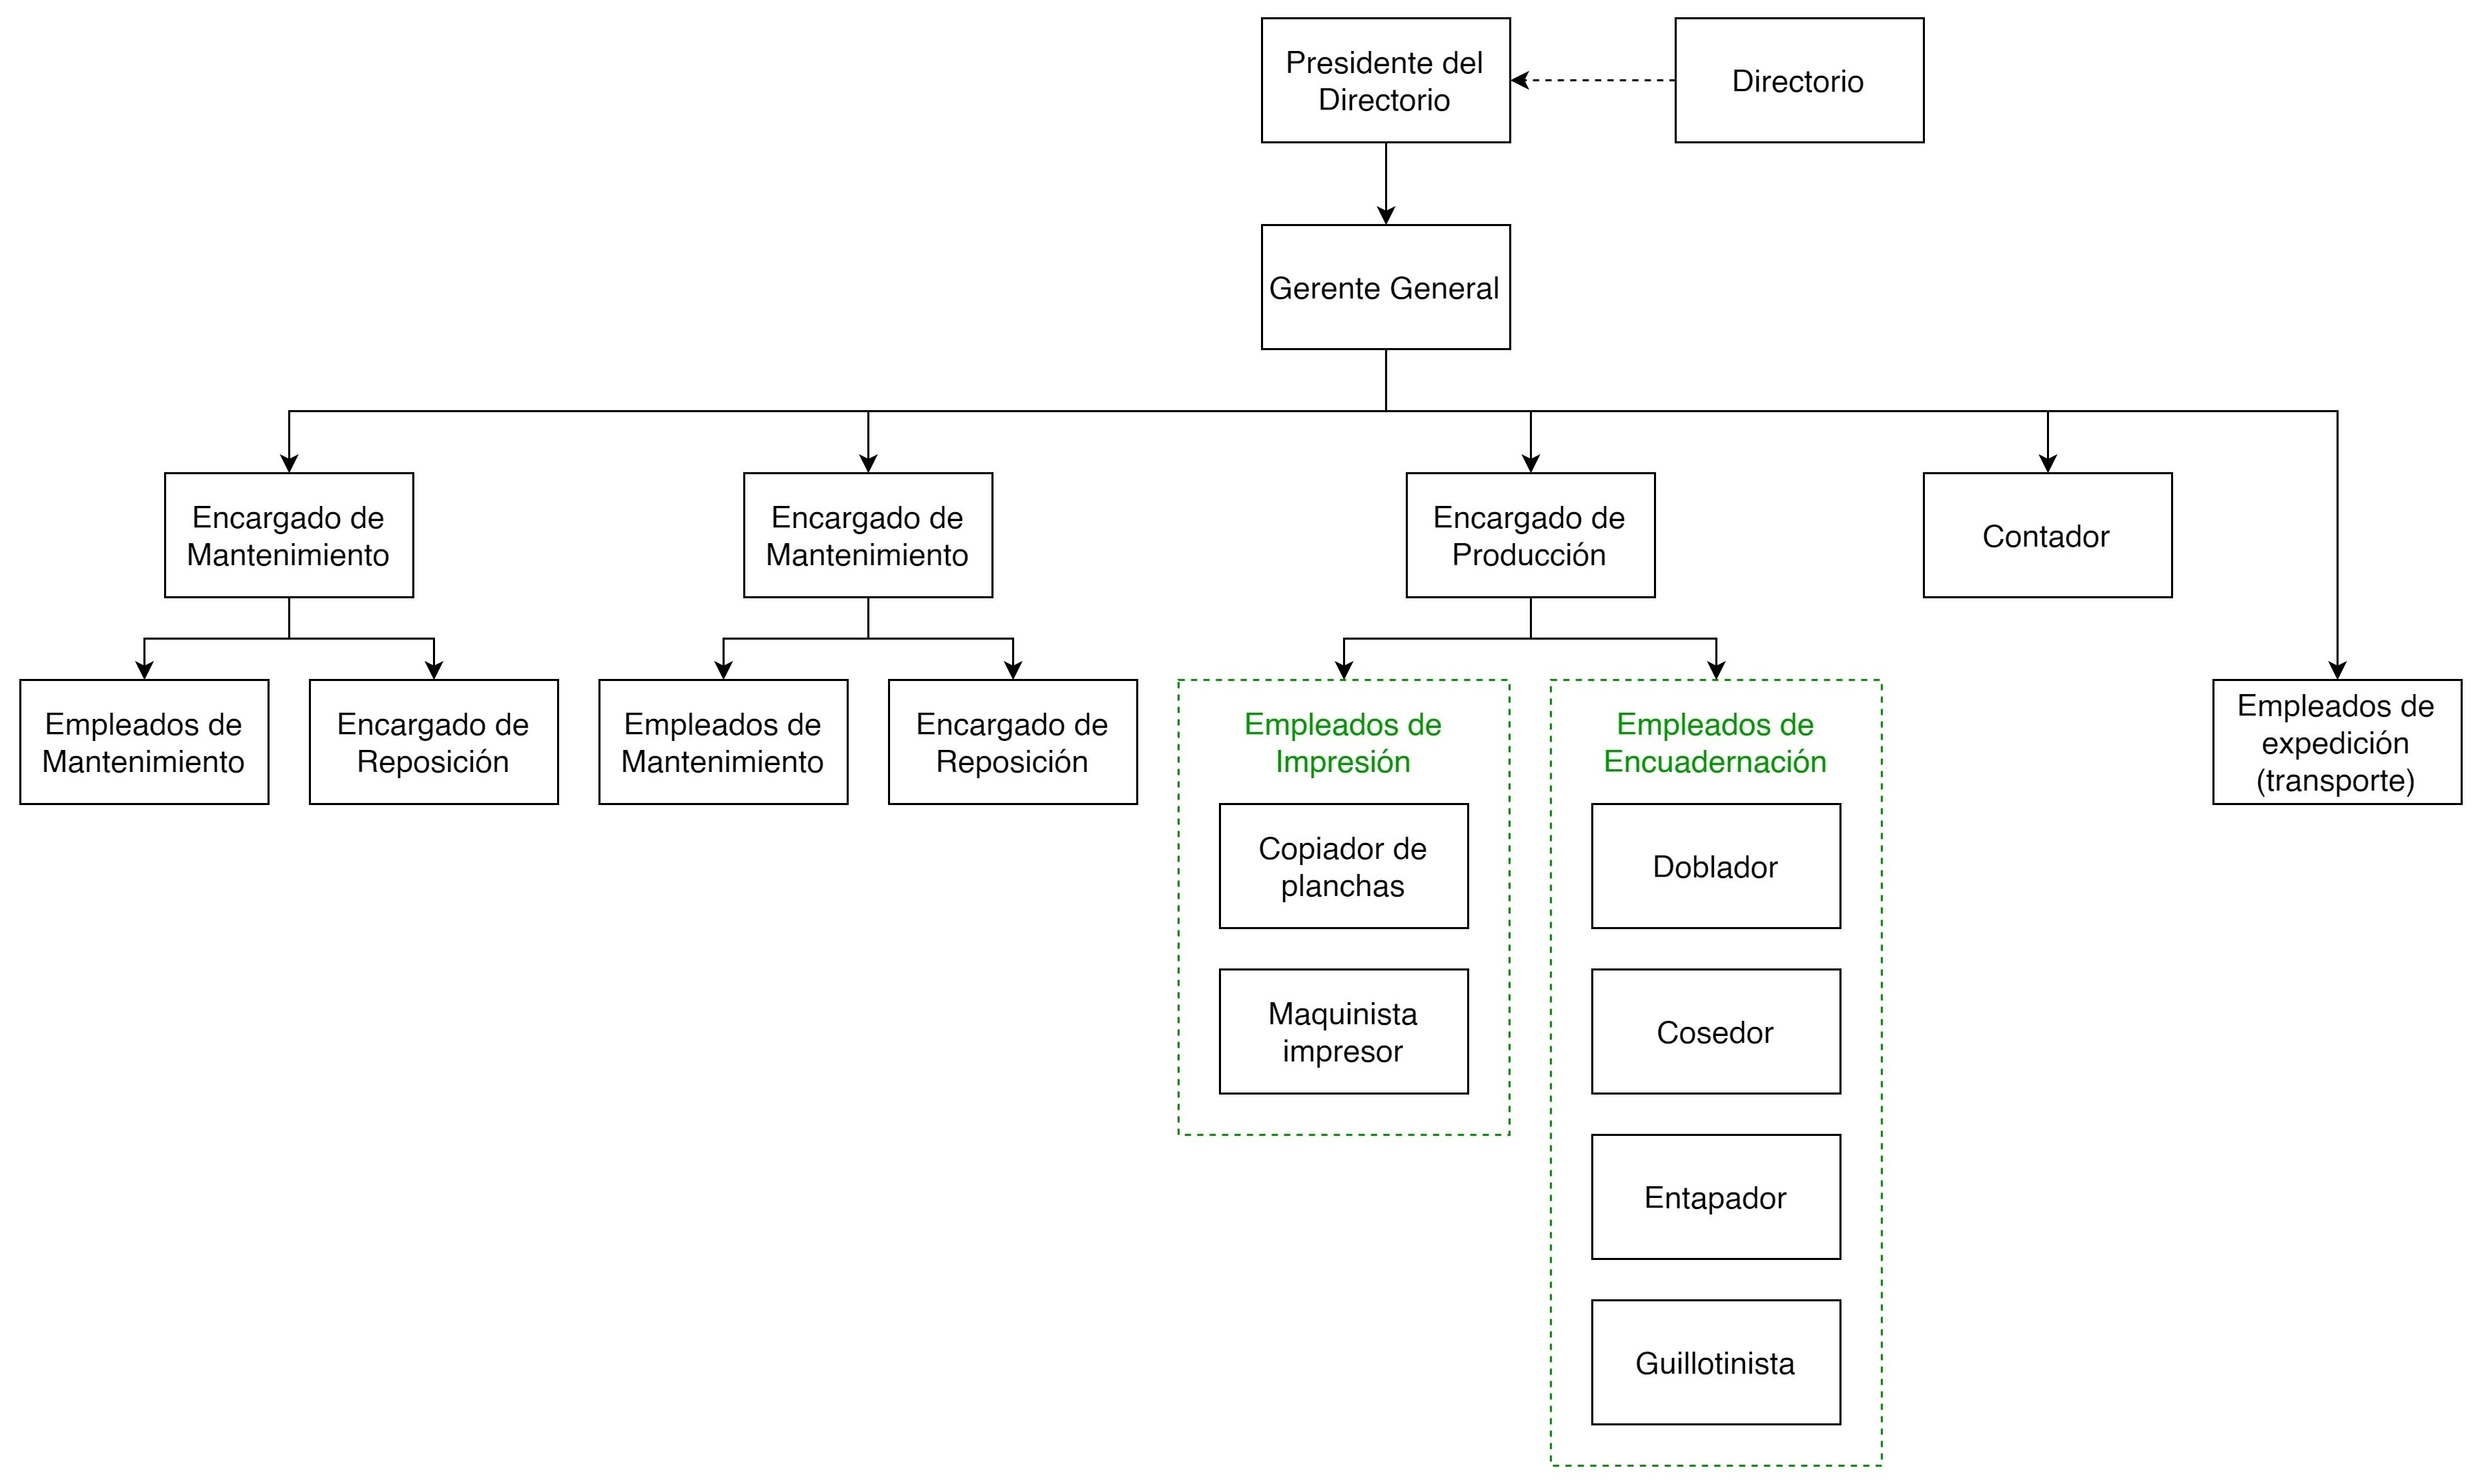
\includegraphics[scale = 0.18]{Organigrama Imprenta Lux.jpg}}%
}%
\caption{Organigrama de Imprenta Lux S.A.}
\label{organigrama}
\end{figure}

\section{Descripción física de la empresa}
\subsection{Divisiones espaciales y emplazamiento}

La empresa cuenta con dos establecimientos diferenciados y separados geográficamente. Ambos cuentan con un depósito cada uno donde se almacenan materiales a cuya gestión será destinado el sistema a desarrollar en el proyecto.
\begin{itemize}
\item El primer establecimiento al cual se denominará <<principal>> tiene fines de gestión así como es donde se realizan algunas tareas sencillas como diagramación, composición, guillotinado, corte y terminación (su depósito correspondiente será denominado <<depósito principal>>).
\colorbox{lightgray}{1- diagramación, composición, copias de planchas (preimpresión). Máquinas de impresión, guillotinas, corte y terminación, alzadora. Talleres de mantenimiento. Depósitos de tintas, reveladores y otros insumos.}
\item El establecimiento restante, al cual denominaremos como <<secundario>> es el relativo a la impresión de los trabajos y donde se realiza la mayor parte del proceso de producción (siguiendo la misma línea, su depósito correspondiente será denominado <<depósito secundario>>).
\colorbox{lightgray}{2- Máquinas de impresión, dobladoras, alzadoras, guillotinas, prensas, cosedoras, cortadora trilateral, embolsadora (termosellado) y expedición (se ponen en cajas los libros) (y una parte es depósito (estanterías de papel que es lo que se va a usar en los próximos días en general)).}
\end{itemize}

 \subsection{Descripción de los depósitos y composición de inventarios}

 \begin{itemize}
 \item Depósito principal: el material en él a su vez se encuentra diferenciado en dos subsectores separados geográficamente en cuartos separados. En el primer cuarto se encuentra el material a ser tenido en cuenta para la gestión de inventario, mientras que el que se encuentra en el segundo cuarto solo tiene fines de picking y sus ingresos y egresos no serán registrados en el sistema, por lo que este segundo subsector puede ser obviado a fines prácticos. El material que se encuentra en ambos cuartos tiene, mayormente, relación con cuestiones de mantenimiento.
\item Depósito secundario: en este espacio se almacenan los materiales que tienen mayor relación con las actividades directas de producción en la empresa, es decir, papeles, tintas, etc.
 \end{itemize}

 \section{Descripción de los procesos de producción} Las tareas que componen los procesos productivos realizados en la empresa difieren en función de los bienes finales, en particular, en base a la producción de cuatro bienes genéricos cuyas secuencias de tareas están mayormente estandarizadas, a saber: libro, revista, almanaque, volante (y afiche).\\
 \indent El proceso de producción inicia cuando los archivos del cliente son recibidos por preimpresión donde se realiza la diagramación, de donde se copian las planchas y se envían a las máquinas de impresión con sus respectivas órdenes (véase fig. \ref{orden taller}) así como a la parte de guillotinado para que el cortador sepa qué material debe cortar, en qué cantidad, tamaño y para qué máquina de impresión. En la medida en que se corta el material, el encargado de impresión carga el papel cortado para realizar su trabajo. Una vez culminada la etapa de impresión, dependiendo del tipo de producto, el material puede ser doblado (por ejemplo en la producción del libro). Luego se intercala, se abrocha o cose si es que correspondiera. En caso de producirse una revista la tapa se intercala y abrocha junto con los pliegos interiores; posteriormente se hace el refilado (guillotinado final para alcanzar el tamaño del producto final). De ser un libro debe prensarse y entaparse para luego pasar por una guillotina trilateral donde se le da el tamaño final. En último término se empaqueta el producto y se deposita en bolsas o cajas según las especificaciones del cliente.

\begin{figure}[h!]
\centering
{%
\setlength{\fboxsep}{0pt}%
\setlength{\fboxrule}{0.5pt}%
\fbox{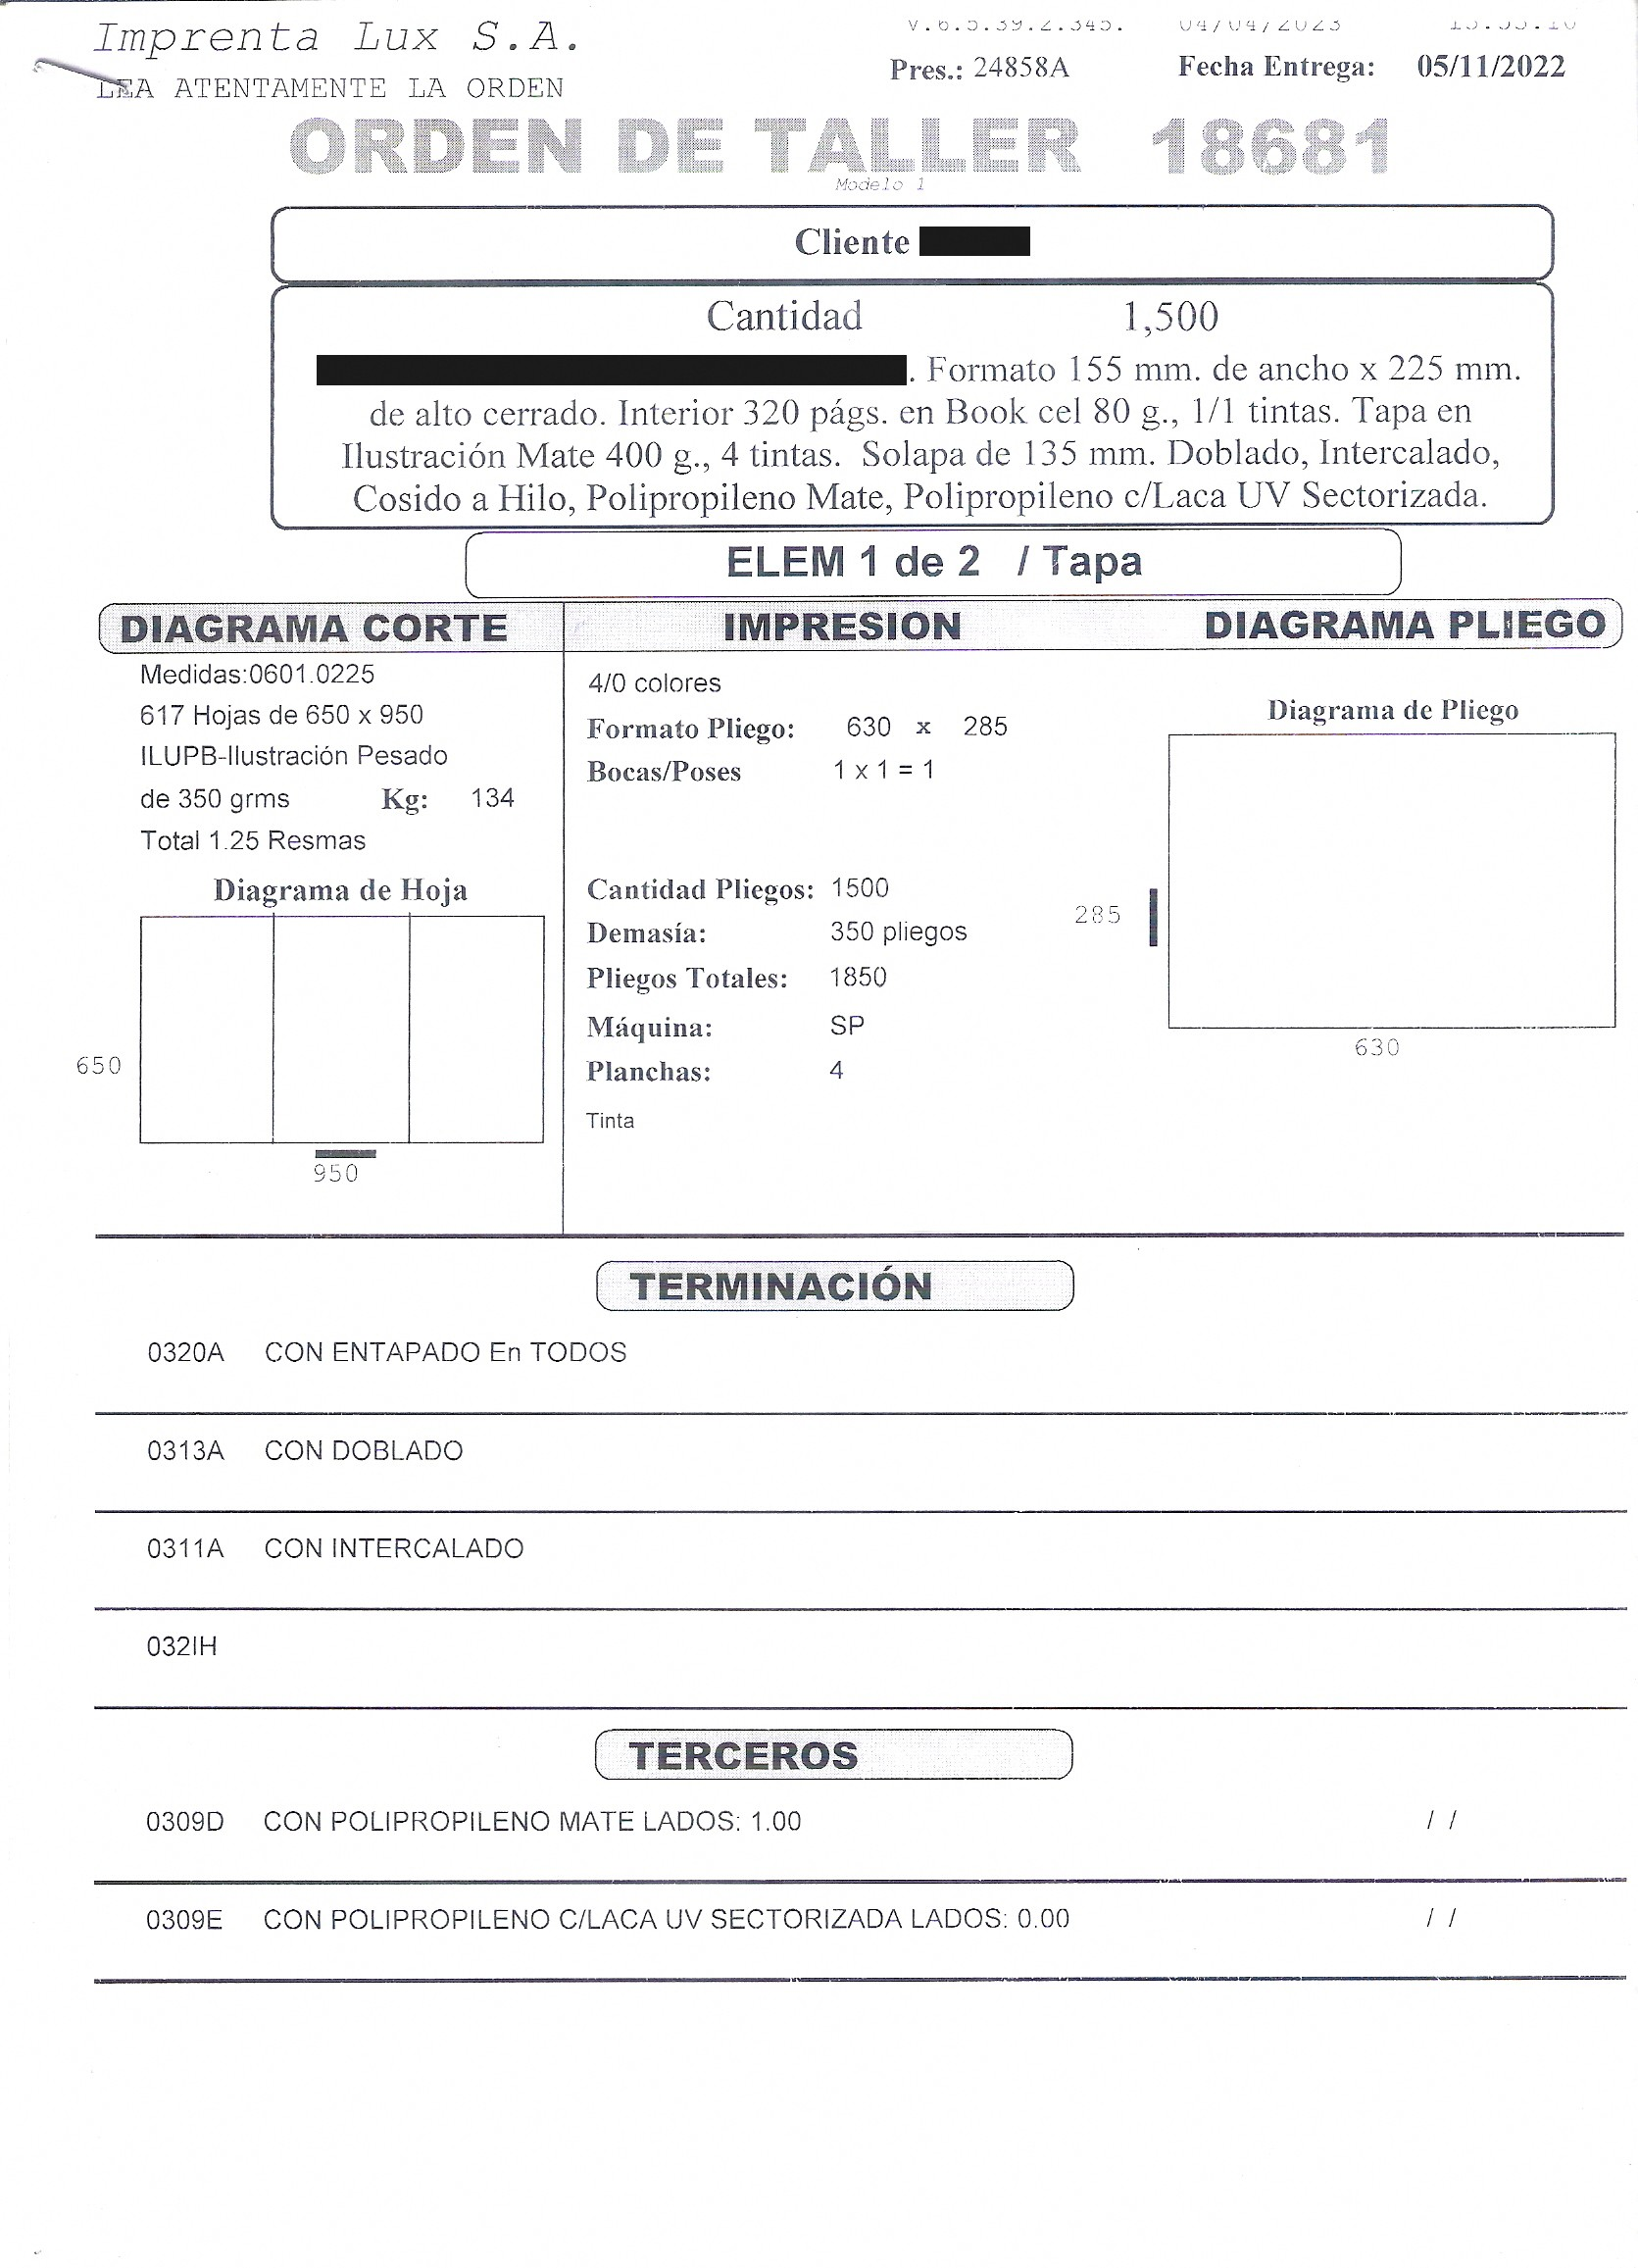
\includegraphics[scale = 0.75]{Orden de taller.jpg}}%
}%
\caption{Orden de taller.}
\label{orden taller}
\end{figure}

\indent En las figuras \ref{diagrama actividad almanaques}, \ref{diagrama actividad libros}, \ref{diagrama actividad revistas} y \ref{diagrama actividad volantes} se muestran los diagramas de actividad de los procesos de producción de almanaques, libros, revistas y volantes/afiches respectivamente.

\begin{figure}[h!]
\centering
{%
\setlength{\fboxsep}{0pt}%
\setlength{\fboxrule}{0.5pt}%
\fbox{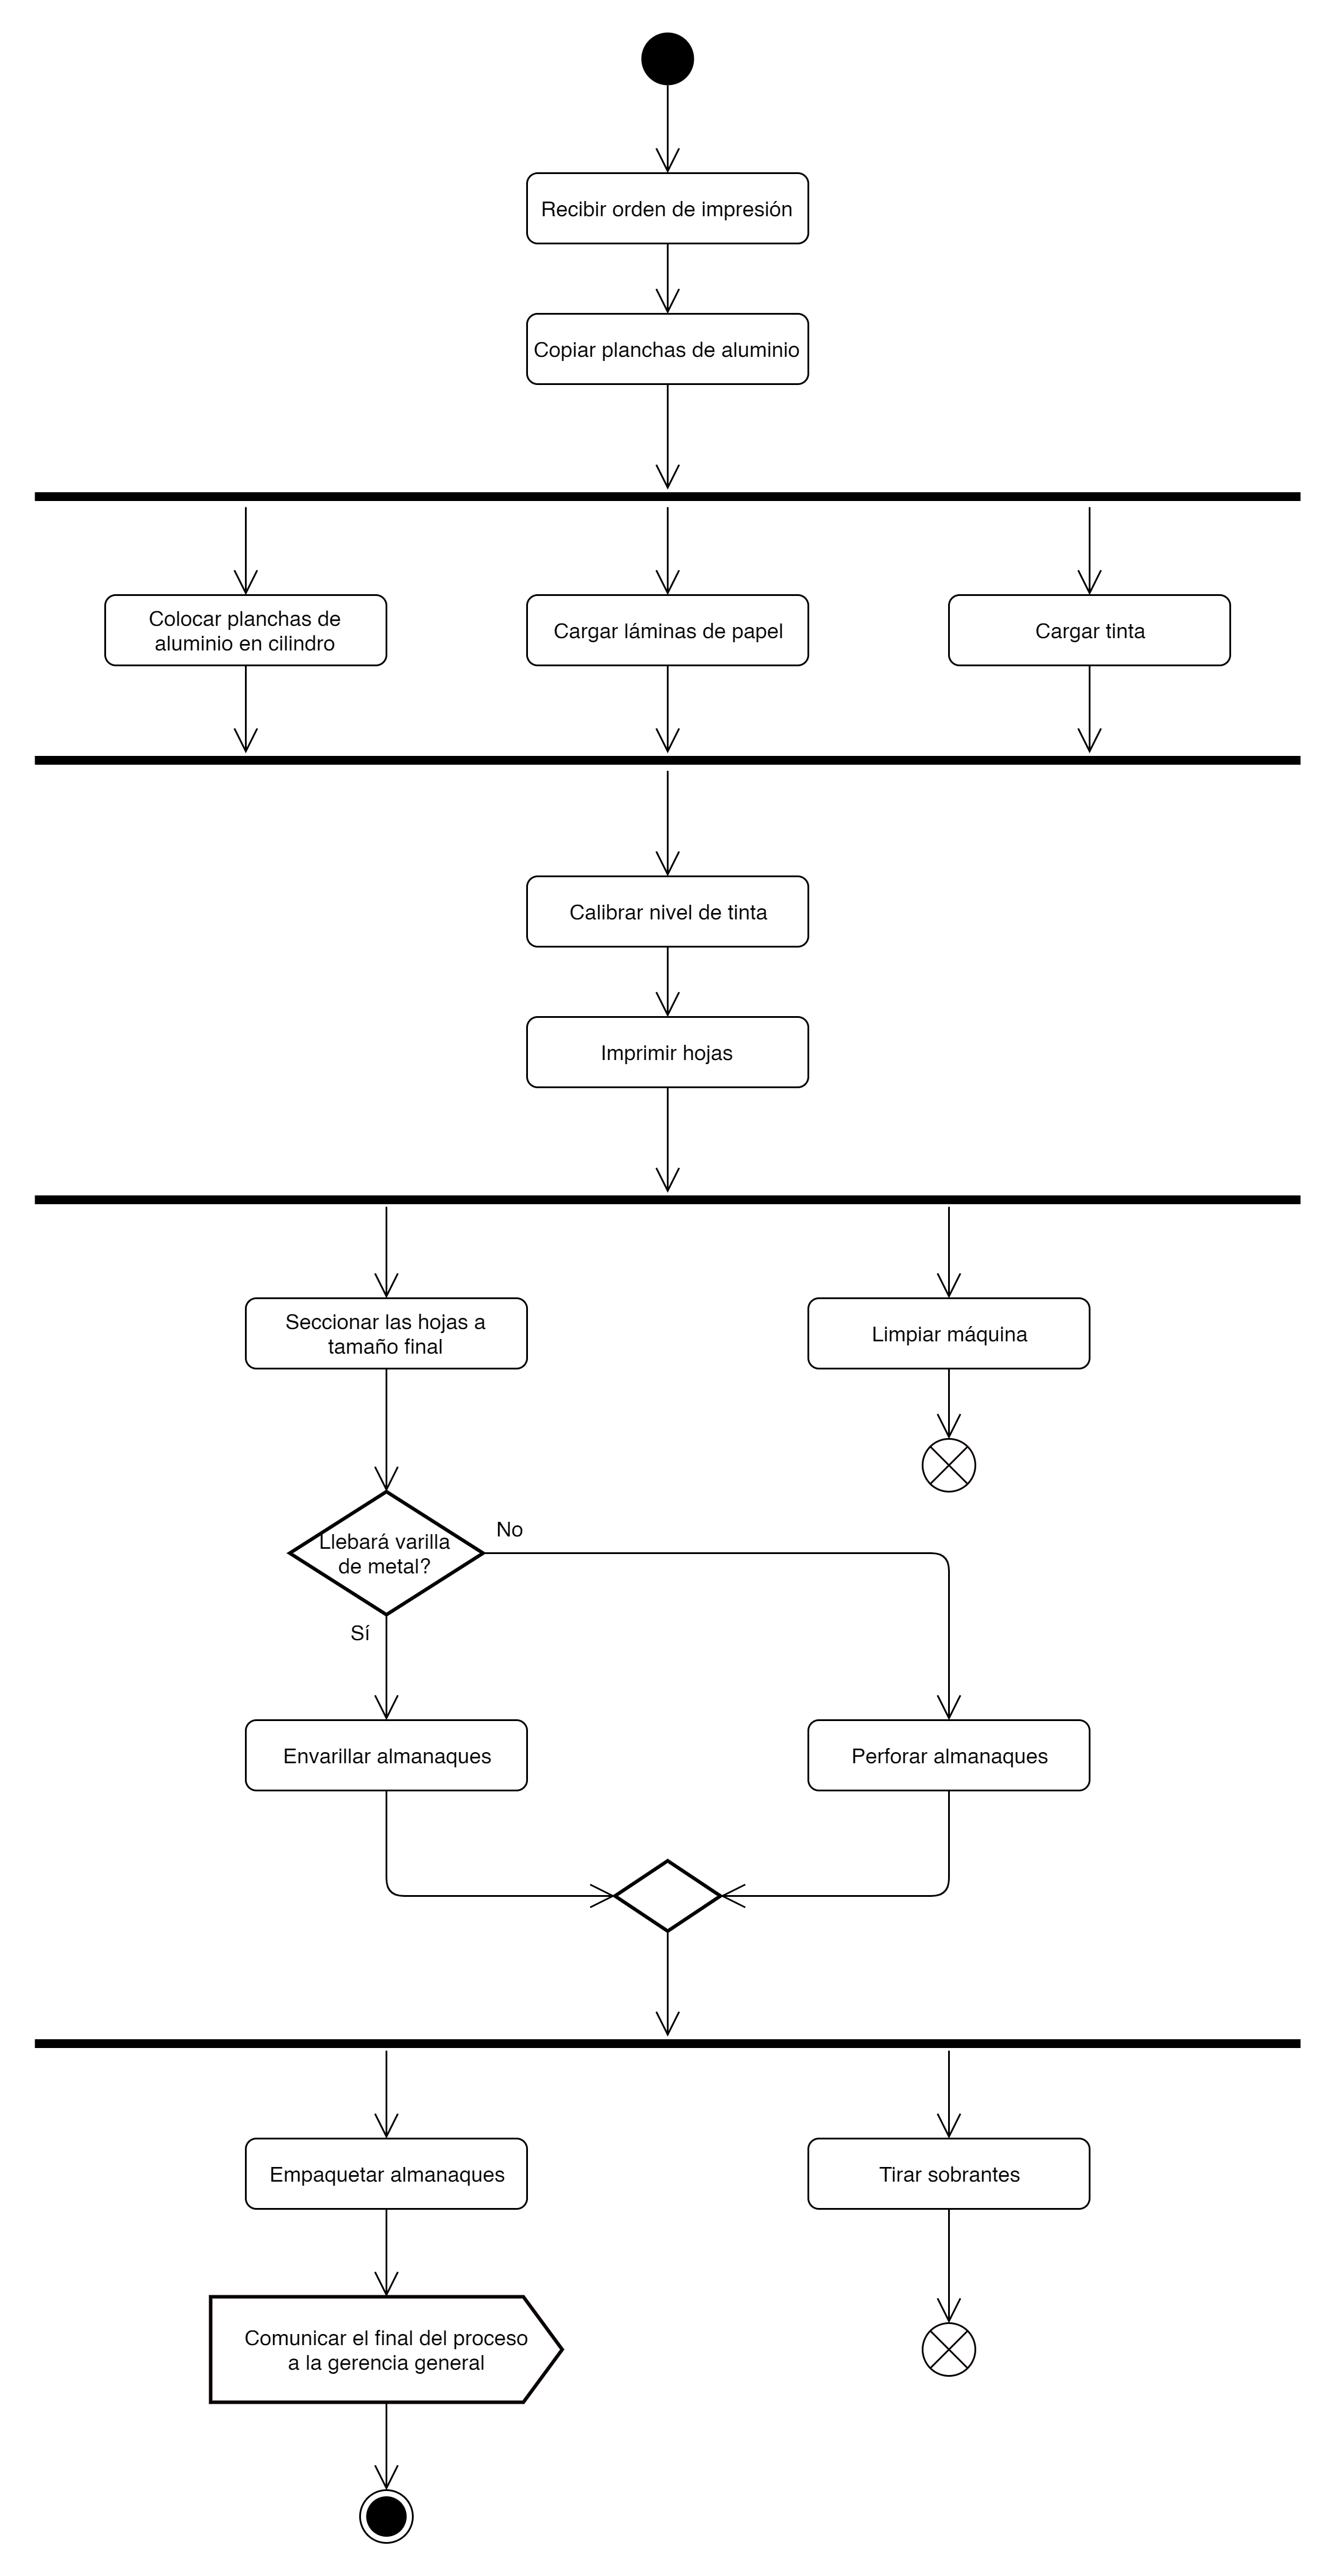
\includegraphics[scale = 0.19]{Diagrama de Actividad Produccion Almanaques.png}}%
}%
\caption{Diagrama de Actividad para Producción de Almanaques.}
\label{diagrama actividad almanaques}
\end{figure}

\begin{figure}[h!]
\centering
{%
\setlength{\fboxsep}{0pt}%
\setlength{\fboxrule}{0.5pt}%
\fbox{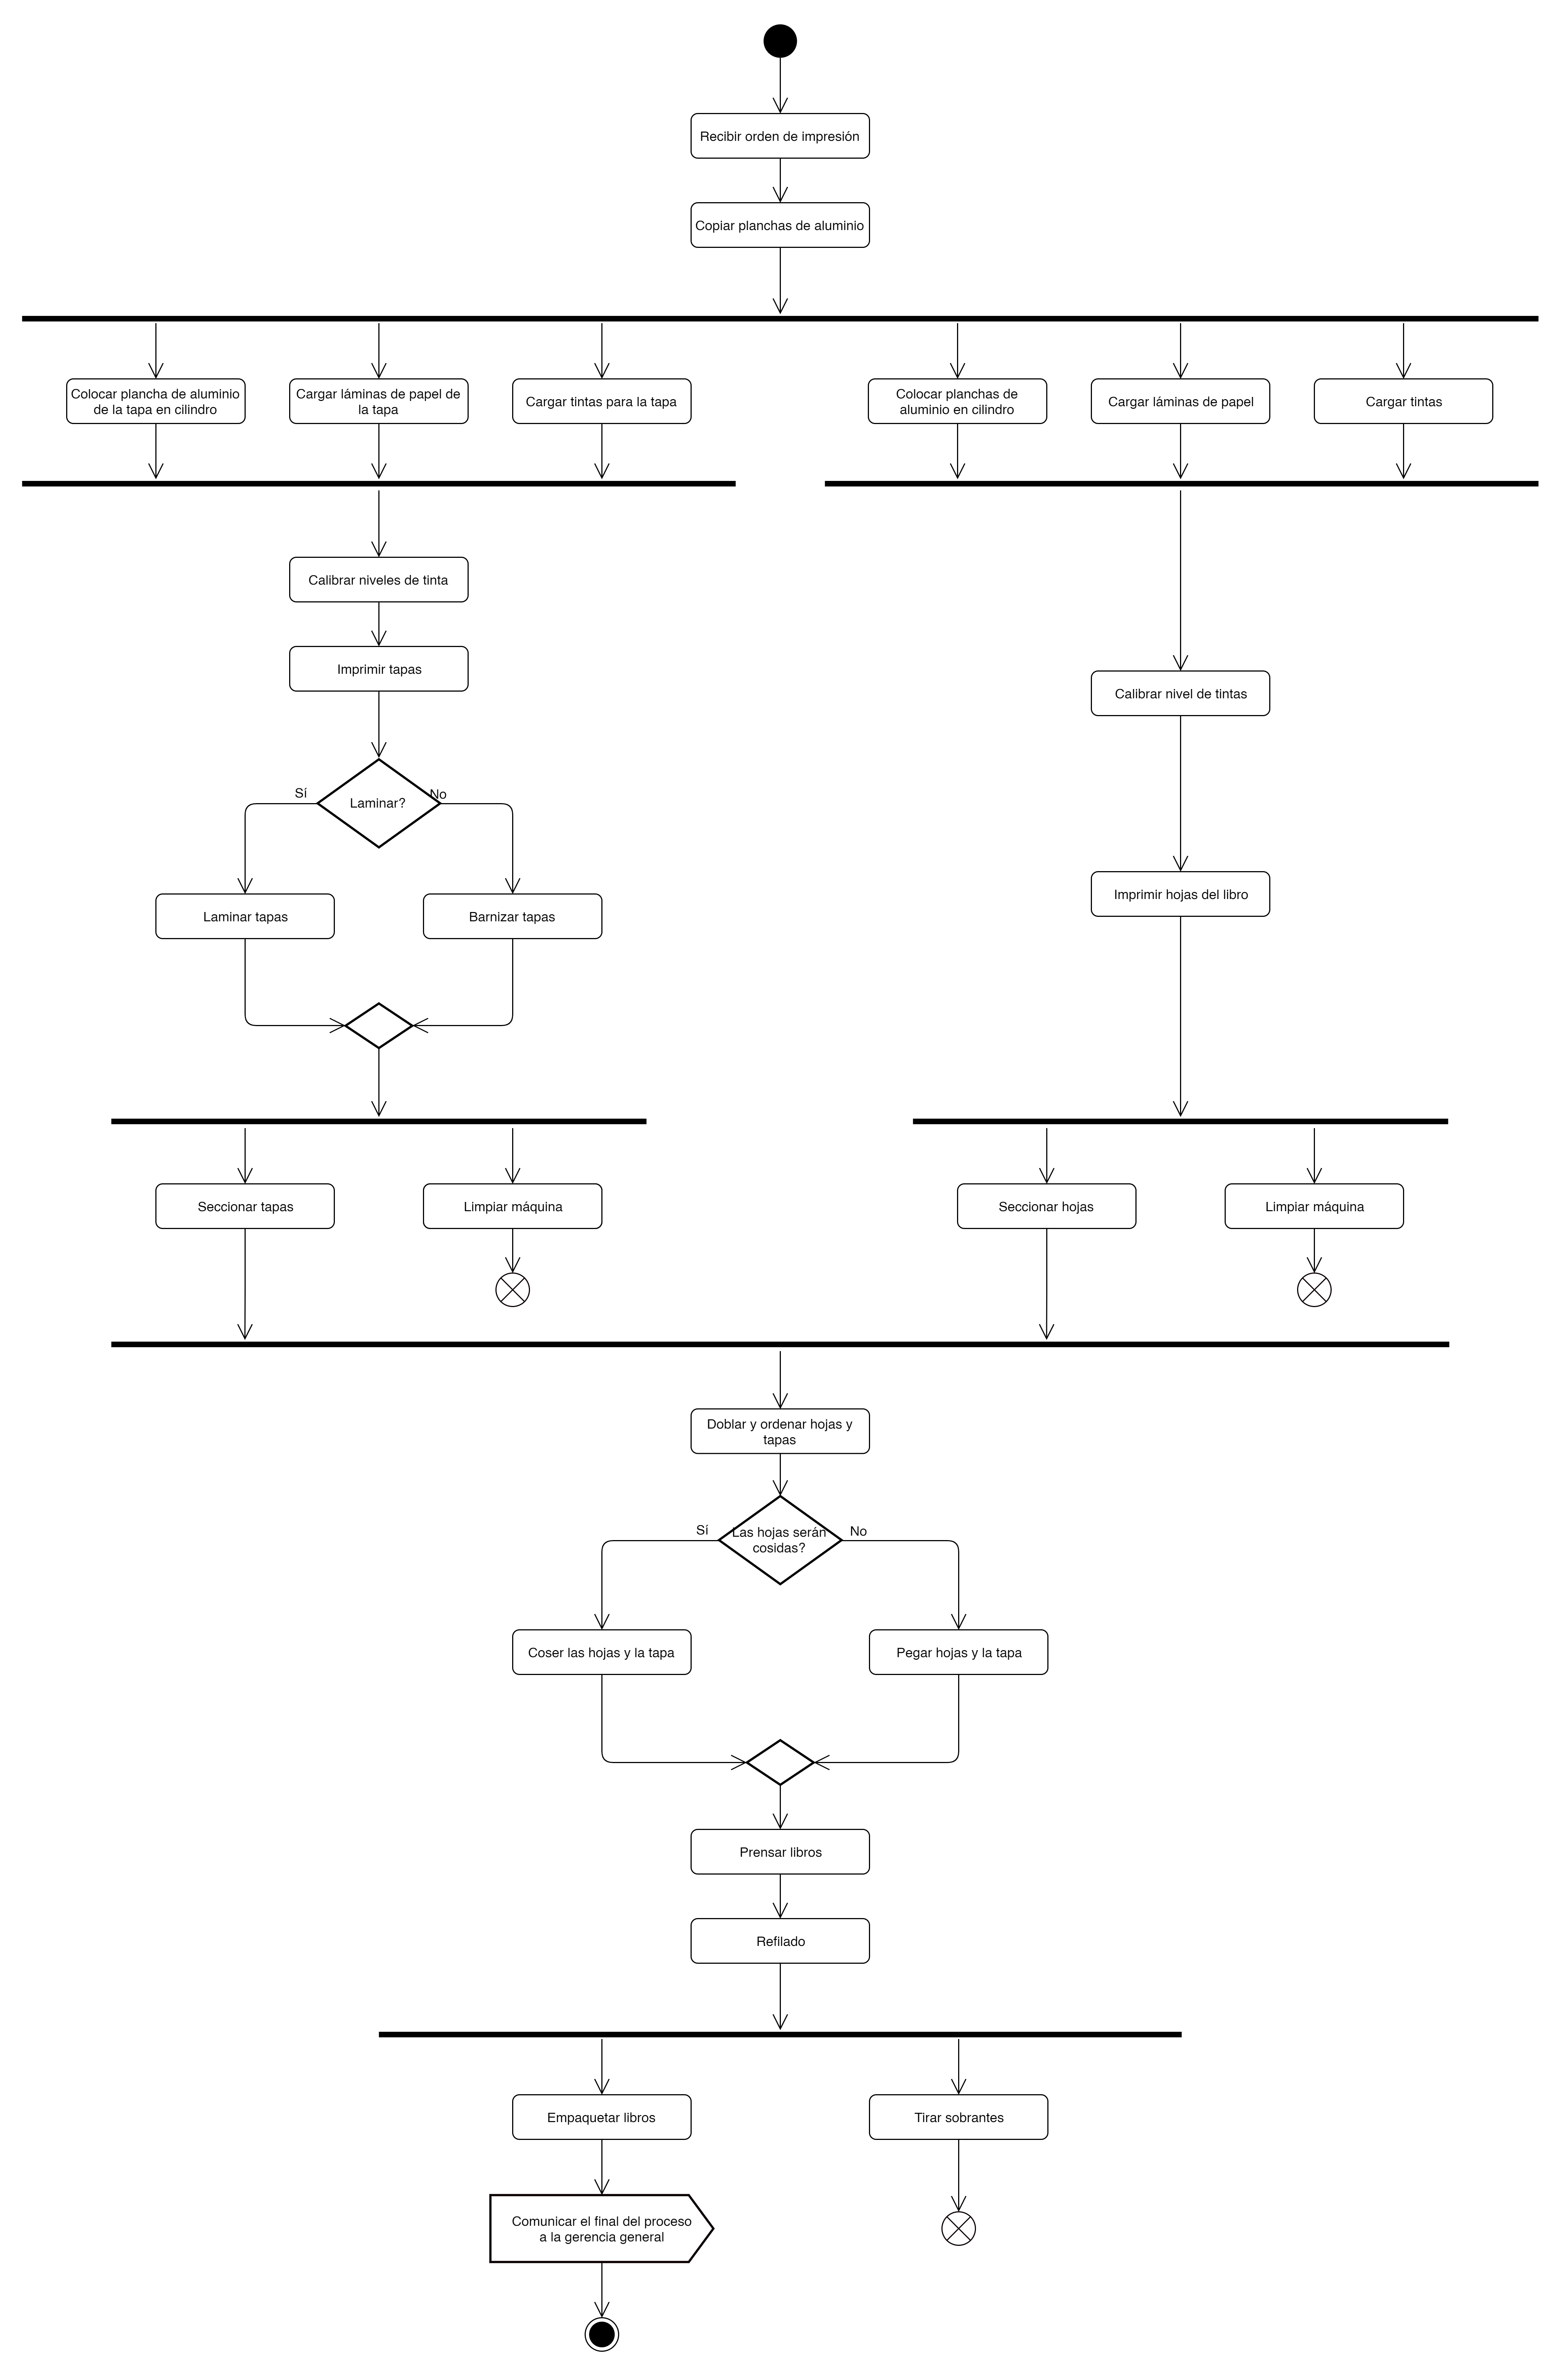
\includegraphics[scale = 0.13]{Diagrama de Actividad Produccion Libros.png}}%
}%
\caption{Diagrama de Actividad para Producción de Libros.}
\label{diagrama actividad libros}
\end{figure}

\begin{figure}[h!]
\centering
{%
\setlength{\fboxsep}{0pt}%
\setlength{\fboxrule}{0.5pt}%
\fbox{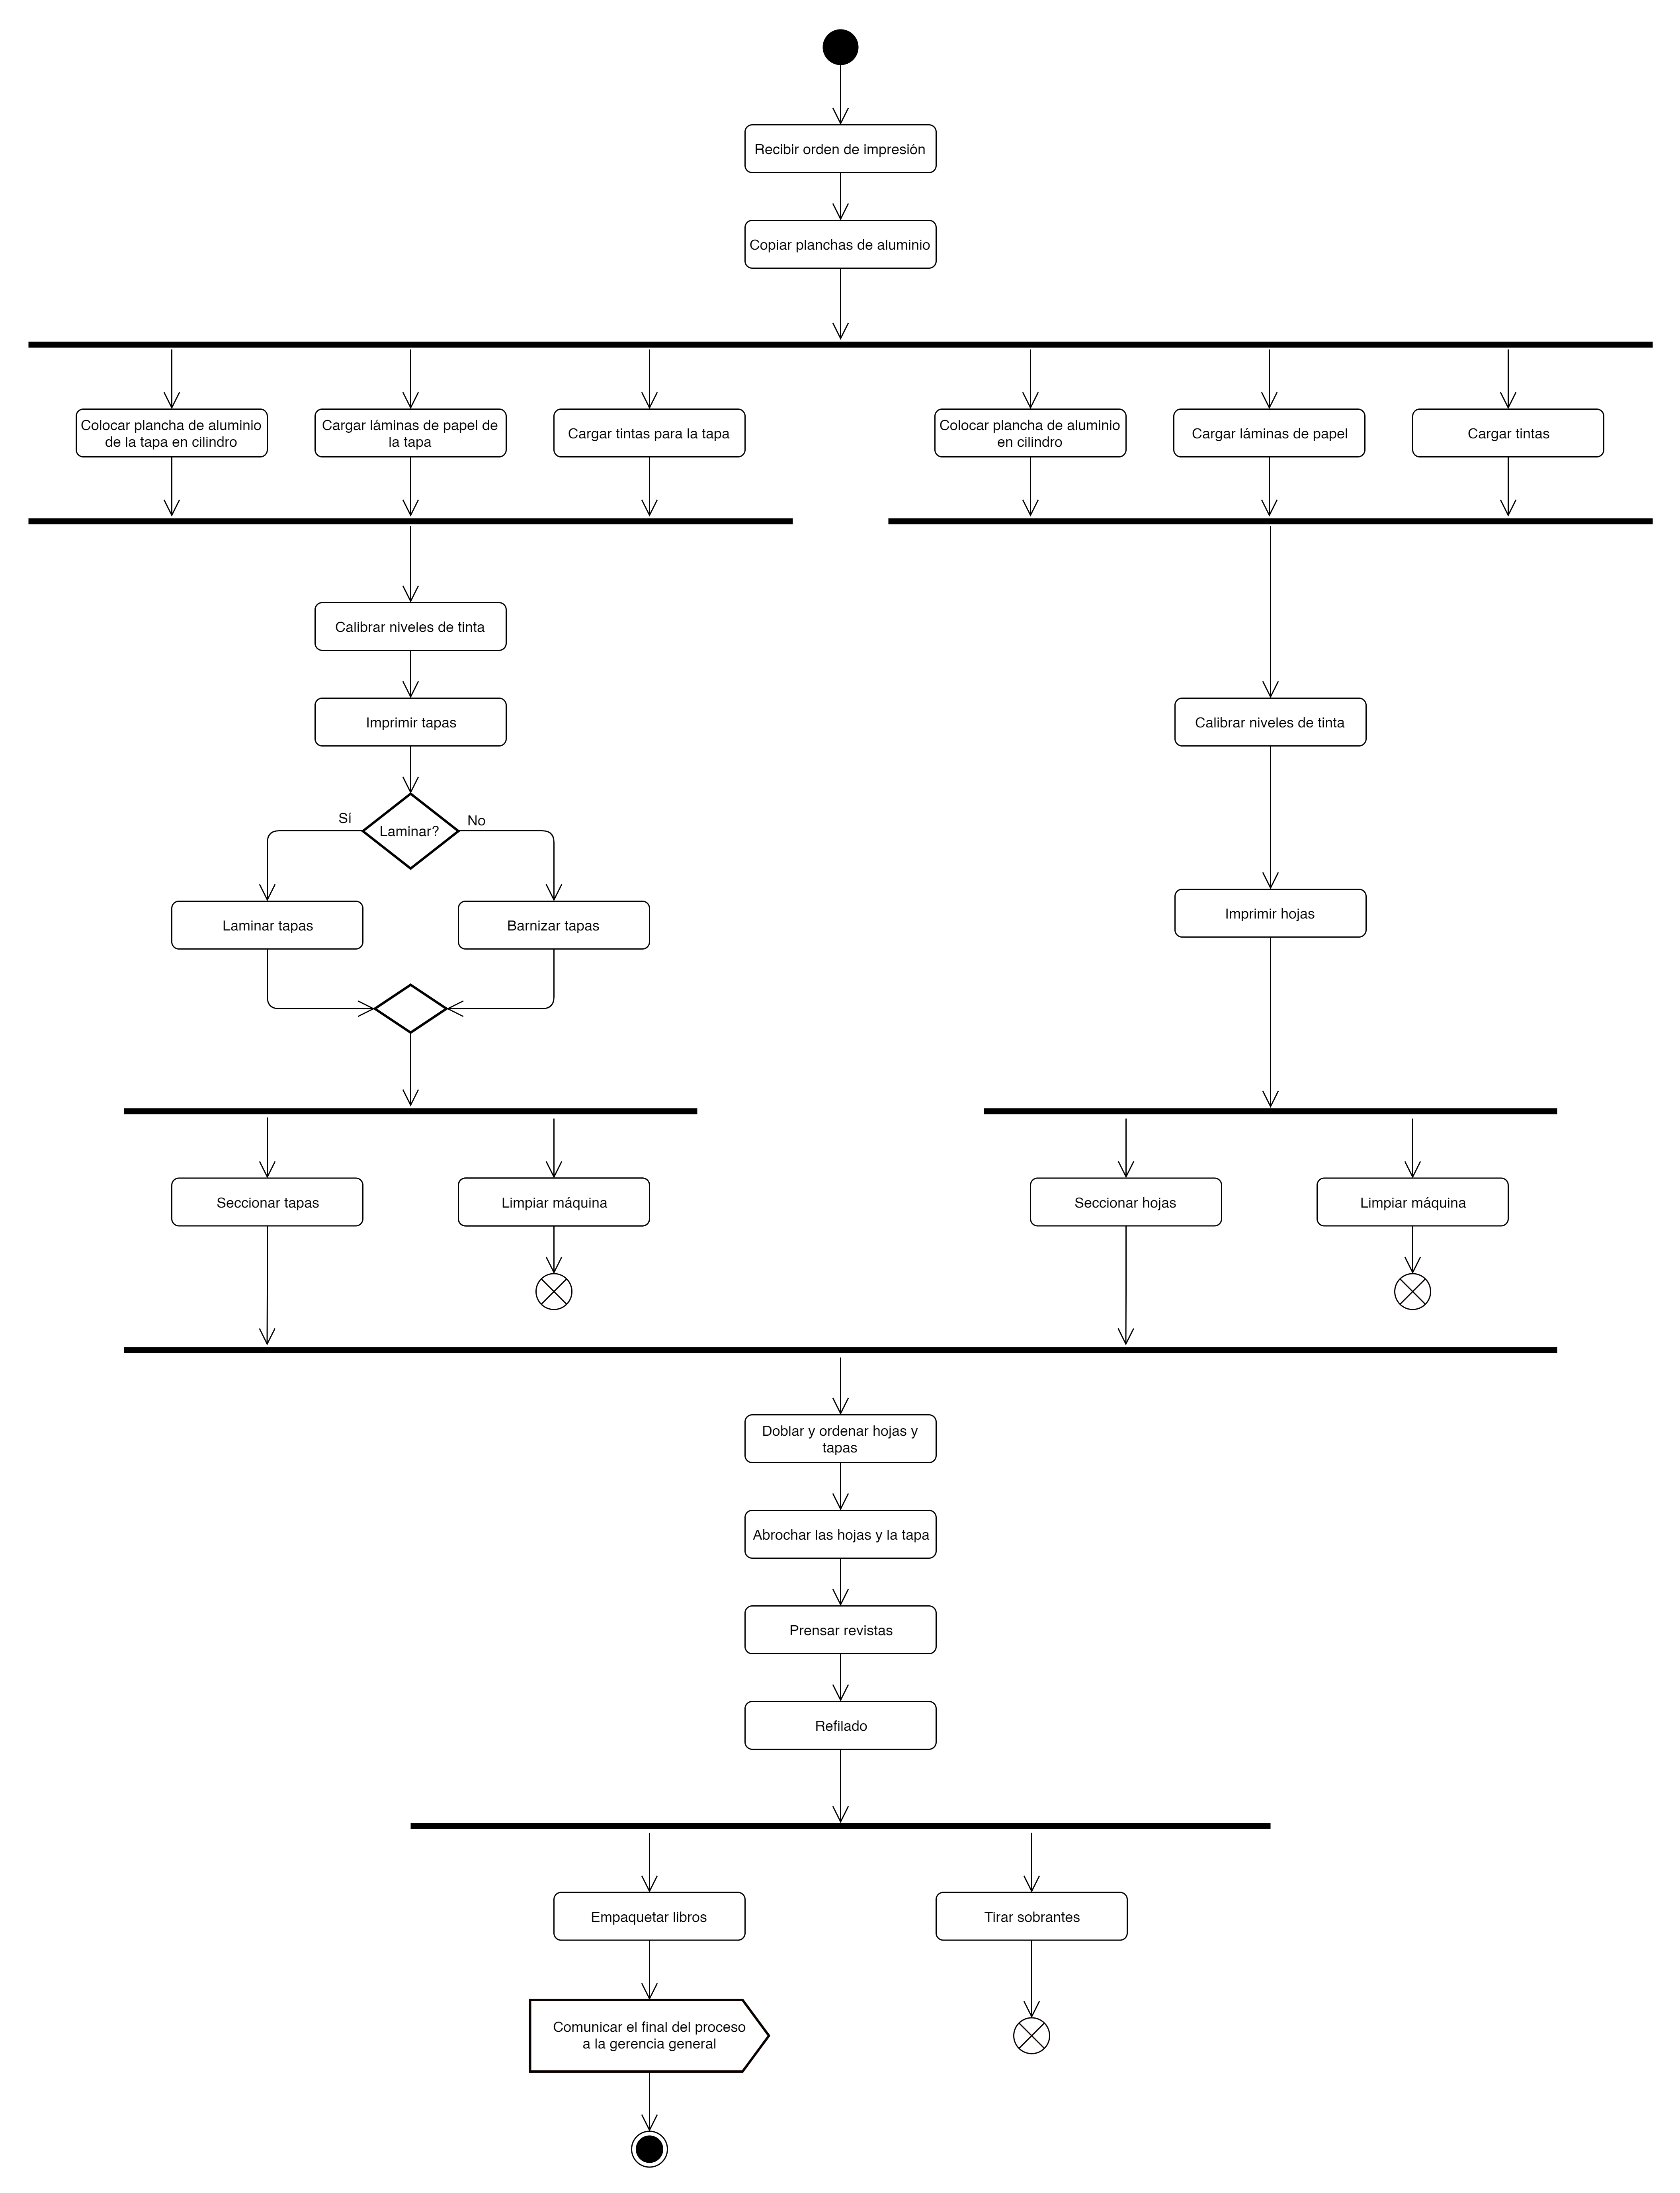
\includegraphics[scale = 0.15]{Diagrama de Actividad Produccion Revistas.png}}%
}%
\caption{Diagrama de Actividad para Producción de Revistas.}
\label{diagrama actividad revistas}
\end{figure}

\begin{figure}[h!]
\centering
{%
\setlength{\fboxsep}{0pt}%
\setlength{\fboxrule}{0.5pt}%
\fbox{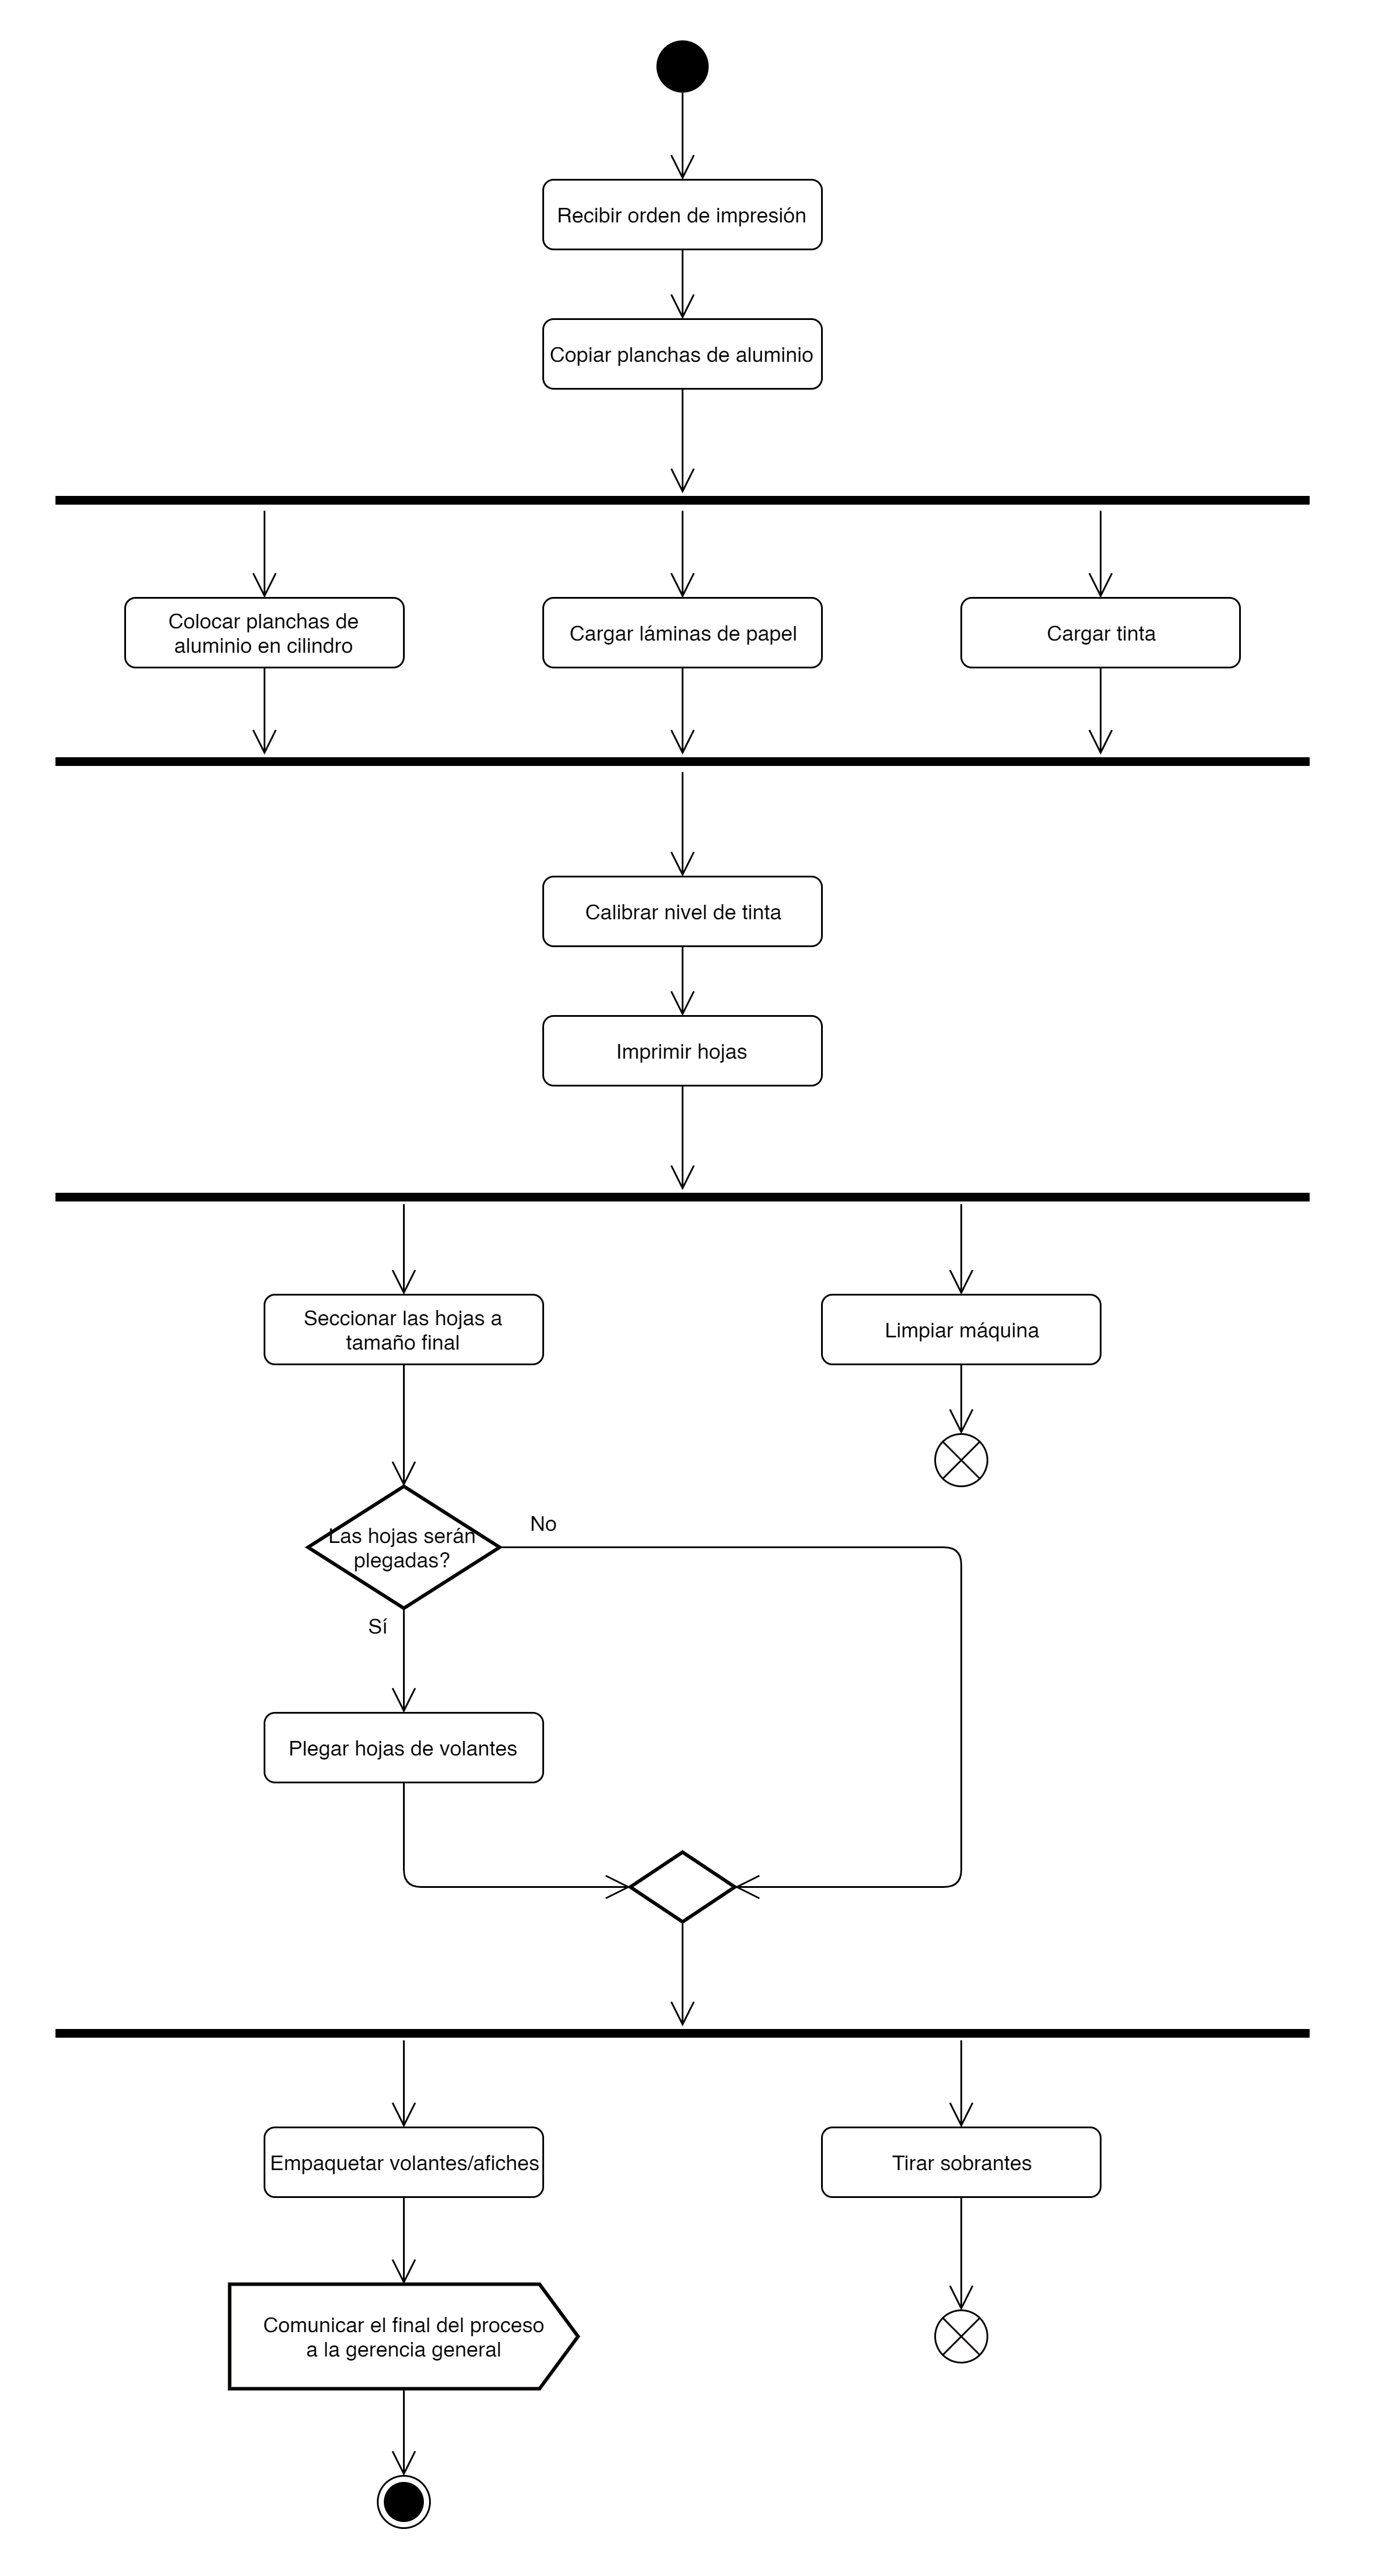
\includegraphics[scale = 0.185]{Diagrama de Actividad Produccion Volantes.png}}%
}%
\caption{Diagrama de Actividad para Producción de Volantes/Afiches.}
\label{diagrama actividad volantes}
\end{figure}

\chapter{Descripción del problema} \label{Descripción del problema}

Podemos dividir el problema general que mediante el proyecto se plantea resolver en dos partes fundamentales diferenciadas, las cuales son: la gestión de los inventarios de la empresa y el control de la producción.

\section{Control de inventarios}

Actualmente al control de insumos\renewcommand*{\thefootnote}{\fnsymbol{footnote}}\footnote[1]{Solo teniendo en cuenta materias primas y materiales de mantenimiento (\hyperlink{MRO}{MRO}: Maintenance, repair, and operations), ya que tanto el inventario de trabajo en proceso (\hyperlink{WIP}{WIP}: Work In Process) como el de bienes finales no forman parte del problema.}\renewcommand*{\thefootnote}{\arabic{footnote}} y relevamiento de depósitos lo realiza el encargado de mantenimiento, sin embargo, no se cuenta con un registro centralizado de los mismos, por lo que es común que se experimenten retrasos en la producción, así como en la toma de decisiones ante el requerimiento de presupuestos y tiempos por parte del cliente, lo cual termina por afectar el trabajo del gerente general. Este último en varias ocasiones no puede estar seguro de las estimaciones de tiempos para los trabajos requeridos ya que para hacerlo debería tener un registro actualizado de los insumos con el que se cuenta en los depósitos, y aún de tenerlo, debería ser posible establecer si dichos insumos, aún disponibles físicamente, no se encuentran ya reservados para ser usados en otros trabajos y se encuentran a la espera de ser utilizados en producción.\\
\indent Además de esto, de no haber una revisión periódica de los inventarios (lo cual parece ser habitual), suele presentarse incluso faltantes de elementos de producción, o no ser posible emitir una orden de compra a tiempo cuando se llegue al \hyperlink{Pp}{Pp} (punto de pedido) de un insumo, lo cual pueden llegar a traducirse en retrasos en los plazos pactados con el cliente para la entrega de determinados trabajos.\\
\indent El control periódico por parte del encargado de mantenimiento, parecería ser la única medida para recabar la información de disponibilidad actualmente debido a que el ingreso de insumos está a cargo del encargado de reposición, quien, como se mencionó, no es quien se encarga del relevamiento de los depósitos.

\section{Control de la producción}

Debido a la separación geográfica de los talleres pertenecientes a la empresa, el encargado de producción debe estar constantemente desplazándose o en contacto con los empleados de producción con el fin de diagramar los trabajos planeados. Del mismo modo, la falta de centralización de la información provoca que, de haber un inconveniente con una máquina de modo que deba pasar a control del equipo de mantenimiento, esto o los retrasos no sean informados sino hasta que fueron resueltos, lo cual termina por dificultar del mismo modo la diagramación de trabajos por parte de los empleados de jerarquías superiores (el mismo encargado de producción o el gerente general). Claramente estas dificultades mencionadas se incrementan en tanto mayor sea el número de trabajos que se estén realizando de manera simultánea.

\chapter{Enfoque de resolución del problema}

Habiendo descrito el problema (véase capítulo \ref{Descripción del problema}), es posible tratar el enfoque de resolución del mismo.\\
\indent Se describirán las características del proyecto así como la metodología de trabajo propuesta para su resolución.

\section{Características generales del proyecto}
\label{Caracteristicas_generales_del_proyecto}
Se tiene una serie de características en la que es posible basarse para la elección de un modelo de procesos adecuado para el software a desarrollar. Se puede mencionar:
\begin{itemize}
	\item Baja cantidad de usuarios y stakeholders en general debido a que se trata de una empresa de un tamaño relativamente pequeño (alrededor de 30 empleados).
	\item El alcance es reducido en relación a otros sistemas empresariales (integra solamente los procesos de control de la producción e inventarios de la empresa).
	\item Requisitos no absolutamente definidos desde el inicio, ya que la empresa no ha trabajado con un sistema de alcance similar al pretendido para el presente sistema.
	\item Equipo de desarrollo pequeño (dos integrantes).
	\item El cliente muestra predisposición y, al menos inicialmente, buena disponibilidad para la comunicación.
\end{itemize}

\section{Modelo de desarrollo del software utilizado}
\label{Modelo de desarrollo del software utilizado}
En base a las características del proyecto mencionadas (principalmente la probabilidad alta de cambios y la posibilidad de comunicación constante con el cliente), se decidió implementar un modelo de desarrollo de software basado en principios generales de las metodologías ágiles conocidas con el fin de obtener los beneficios que de la utilización de éstas se desprenden. En relación a lo anterior, se considera que en este caso no es posible la adopción plena de una metodología ágil predefinida a causa del bajo número con el que cuenta el equipo de desarrollo; esto afecta directamente características con la que cuentan metodologías como Scrum, la cual define distintos roles, o por ejemplo la práctica de \textit{Pair Programming} originaria de XP, la cual de aplicarse aumentaría considerablemente el tiempo necesario de trabajo para finalizar las tareas previstas.\\
\indent Las premisas, por lo tanto, en las que se decidió basarse (determinadas directamente como base de las metodologías ágiles o que vienen como consecuencias de éstas) para la realización del presente proyecto son las mencionadas a continuación\footnote{Estos principios se basan en las descripciones presentadas en:\\ \indent <<\textit{Manifesto for Agile Software Development}>> de Agile Manifesto, \url{http://agilemanifesto.org/}. Consultado el 11/04/2024;\\ \indent <<\textit{The 12 Principles behind the Agile Manifesto}>> de Agile Alliance, \url{https://www.agilealliance.org/agile101/12-principles-behind-the-agile-manifesto/}. Consultado el 11/04/2024;\\
	\indent Kumar, Gaurav - Bhatia, Pradeep K. \textit{<<Impact of Agile Methodology on Software Development Process>>}. International Journal of Computer Technology and Electronics Engineering (IJCTEE)
	Volume 2, Issue 4, Agosto 2012. Págs. 46-47.}:
\begin{itemize}
	\item \underline{Comunicación constante con el cliente:} para una mejor comprensión del problema así como en pos de no incurrir en asunciones erróneas que puedan traducirse en futuros cambios que produzcan pérdidas de tiempo que podrían utilizarse en aumentar la calidad final del producto, así como en adiciones involuntarias de fallos técnicos (ya sea de funciones particulares o, peor aún, estructurales del sistema) por modificaciones del código.
	\item \underline{Im\smash{p}lementación de \smash{p}rácticas de forma iterativa:} la adaptabilidad del software a modificaciones imprevistas por parte del cliente permite que estas últimas puedan ser realizadas en un plazo corto (estipulado de entre algunas semanas a algunos meses) sin extender las consecuencias de una implementación que no se condiga con lo esperado. Esto es relativo tanto a requerimientos adicionales como a modificaciones de los requerimientos del software producido o a producir. Al mismo tiempo, debido a que no se espera hasta el final de la implementación para validar el producto, de acuerdo a las modificaciones propuestas en cada etapa/iteración, se adquiere una mejor perspectiva en cuanto a las expectativas del proyecto, así como una medición constante del progreso y aceptación de los desarrollos parciales.
	\item \underline{Reducida documentación con ma\smash{y}or atención a la calidad del software:} la reducida documentación motiva a los miembros del equipo de trabajo a enfocarse en la calidad del producto, reduciendo al mismo tiempo las cargas producidas por excesivas actividades de documentación. De cualquier modo, es importante destacar que, a pesar de esto, no se está sugiriendo una ausencia total de documentación, sino de evitar realizar excesiva documentación para dar prioridad a la calidad del software implementado.
\end{itemize}

\section{Metodología de desarrollo y coordinación del equipo}

Se considera que, a pesar de haberse optado por la adopción de un método de desarrollo basado en los principios ágiles, no existe un modelo predefinido al cual sea posible adecuarse completamente  (véase capítulo \ref{Modelo de desarrollo del software utilizado}). Por esto, se describe a continuación la metodología de trabajo particular que se implementa en este caso:\\
\indent Inicialmente se opta por hacer una primera aproximación de la solución mediante reuniones con el cliente donde se definen a grandes rasgos los requerimientos del sistema. Tales requerimientos son plasmados de manera resumida en forma de historias de usuario (\hyperlink{US}{US}, las cuales se muestran en el \hyperlink{apendice_a}{Apéndice A} con sus respectivos refinamientos).\\
\indent Teniéndose las \hyperlink{US}{US} definidas (pueden no ser la totalidad de las mismas a lo largo del proyecto), los miembros del equipo de desarrollo las refinan de modo de detallarlas en forma de tareas o \textit{<<tasks>>}. A su vez, en la medida en que surgen dudas respecto a aspectos no tratados en las reuniones con el cliente, se genera una lista de preguntas para ser planteadas a este último.\\
\indent La estimación de esfuerzo (tiempo de trabajo) para las \hyperlink{US}{US} definidas se hacen mediante la asignación de \textit{<<points>>} a las mismas, las cuales son relativas entre unas y otras, de modo que mayor cantidad de points serán asignados a la \hyperlink{US}{US} que se crea pueda tener más costo de desarrollo. Las \hyperlink{US}{US} más sencillas se pueden tomar de referencia, y de acuerdo a sus estimaciones y de forma proporcional a las de mayor complejidad, ser utilizadas para estimar el esfuerzo de estas últimas.\\
\indent A partir de las asignaciones relativas mencionadas, se define la \textit{<<velocidad>>} de trabajo medida en \textit{tiempo/point}. De este modo, habiendo asignado los points a las \hyperlink{US}{US} definidas y establecida la velocidad, es posible estimar el tiempo real de trabajo para cada \hyperlink{US}{US} de manera individual.\\
\indent Se debe seleccionar un tamaño de iteración (\textit{Iteration Size}), que no es más que el tiempo que durará cada iteración o \textit{<<Sprint>>}.\\
\indent Las \hyperlink{US}{US} se identifican en base a la importancia de negocio así como a la prioridad de desarrollo con el fin de poder establecer un orden de implementación acorde (aunque finalmente, como se menciona en la subsección \ref{requerimientos_del_sistema_e_historias_de_usuario}, ya que el proyecto consta de un solo release, se optó por una prioridad basada únicamente en la dependencia de desarrollo de las \hyperlink{US}{US}). En relación a esto se seleccionan las \hyperlink{US}{US} a implementar por iteración, teniéndose siempre presente que no será posible seleccionar más \hyperlink{US}{US} que las que puedan implementarse de acuerdo a la velocidad estimada.\\
\indent Ya que lo que se intenta es que las estimaciones de los points asignados a las \hyperlink{US}{US} guarden una correcta proporción en cuanto a sus complejidades relativas, así como no introducir más errores humanos al añadir otra posible fuente de error debido a otra estimación basada en la subjetividad del equipo de desarrollo, la velocidad de desarrollo del equipo (cantidad de points finalizados/iteración) será tomada en una iteración dada en función de lo evidenciado en la precedente. Es decir, la velocidad del equipo no puede superar a la obtenida en la práctica en la iteración anterior. Esto, claro está, no puede ser aplicado a la iteración I, para lo que no queda alternativa a la de asignar una velocidad inicial basada en la experiencia del equipo de desarrollo.\\
\indent Luego de planificada la iteración, los miembros del equipo de desarrollo se dividen las \hyperlink{US}{US} (o incluso las tasks) que cada uno desea implementar.\\
\indent\colorbox{orange}{Seguir...}

\section{Descripción general de la solución planteada}
\indent\colorbox{orange}{Hacer...}

\chapter{Ejecución del proyecto}
\section{Etapa de análisis inicial}

Para la definición del sistema a desarrollar se trabajó con los futuros usuarios del sistema con el objetivo inicial de establecer los requisitos del mismo. En particular, debido a que los stakeholders de mayor jerarquía en la organización son los principales interesados en su uso, y quienes mayores certezas tienen respecto al sistema requerido, se mantuvo una comunicación periódica con los mismos, a saber: la gerente general, el encargado de mantenimiento/control de reposición de la empresa, y el encargado de producción.\\
\indent De lo anterior se obtuvieron las definiciones que se describen a continuación.

\subsection{Requerimientos del sistema e historias de usuario}
\label{requerimientos_del_sistema_e_historias_de_usuario}
Las \hyperlink{US}{US} definidas inicialmente se listan en la tabla \ref{tabla_dependencias_iniciales_us} a modo de resumen con sus respectivas dependencias de desarrollo (para un mayor detalle en cuanto a los refinamientos correspondientes de las \hyperlink{US}{US}, véase el \hyperlink{apendice_a}{Apéndice A}). En este caso particular, debido a que el proyecto consta de un solo release, la prioridad en cuanto al valor de negocio puede ser obviada. Con esta metodología de priorización de \hyperlink{US}{US} se intentó facilitar las tareas de integración al reducir la utilización de componentes de tipo Stub.

\begin{table*}[h!]
\centering
\begin{tabular}{ |p{0.5cm}|p{9cm}|c|  }
\hline
\verb|#|& \textbf{Nombre de \hyperlink{US}{US}}& \textbf{Dependencia} \\
\hline
\textbf{1} & Inicio de sesión & - \\
\hline
\textbf{2} & Administrar usuarios & 1 \\
\hline
\textbf{3} & Administrar insumo & 4 \\
\hline
\textbf{4} & Administrar tipo de insumo & 1 \\
\hline
\textbf{5} & Modificar cantidad de insumo & 3 y 6 \\
\hline
\textbf{6} & Administrar depósitos & 7 \\
\hline
\textbf{7} & Administrar sucursales & 1 \\
\hline
\textbf{8} & Administrar proyecto & 10 \\
\hline
\textbf{9} & Agregar insumo a proyecto & 8 y 3 \\
\hline
\textbf{10} & Administrar tipos de proyectos & 1 \\
\hline
\textbf{11} & Editar tarea & 8 \\
\hline
\textbf{12} & Asignar tarea a empleado & 11\\
\hline
\textbf{13} & Agregar comentario a tarea & 12 \\
\hline
\textbf{14} & Modificar estado de tarea & 11 \\
\hline
\textbf{15} & Finalizar proyecto & 8 \\
\hline
\textbf{16} & Buscar proyecto & 8 \\
\hline
\textbf{17} & Visualizar tareas asignadas & 12 \\
\hline
\textbf{18} & Administrar clientes & 1 \\
\hline
\end{tabular}
\caption{Dependencias de desarrollo entre las \protect\hyperlink{US}{US} definidas.}
\label{tabla_dependencias_iniciales_us}
\end{table*}

\indent Lo anterior puede a su vez visualizarse en la figura \ref{diagrama_dependencias_US}, donde se muestra un diagrama con las dependencias señaladas en la tabla \ref{tabla_dependencias_iniciales_us}.

\begin{figure}[h]
\begin{center}
	\setlength{\fboxsep}{10pt} % Ajusta el padding
	\fbox{
	\begin{tikzpicture}[scale=1.1]
		\GraphInit[vstyle=Normal]
		\SetVertexNormal[Shape=circle,LineWidth = 1pt]
		\tikzset{EdgeStyle/.append style = {color = blue!70, line width=1pt}}
		\renewcommand*{\VertexLineWidth}{1pt}%vertex thickness
		\renewcommand*{\EdgeLineWidth}{1pt}% edge thickness
		\GraphInit[vstyle=Normal]
		
		\Vertex[LabelOut,Lpos=270,L=$us_1$,x=0,y=4]{R1}
		
		\Vertex[LabelOut,Lpos=270,L=$us_2$,x=2,y=8]{R2}
		\Vertex[LabelOut,Lpos=270,L=$us_7$,x=2,y=6]{R7}
		\Vertex[LabelOut,Lpos=270,L=$us_4$,x=2,y=4]{R4}
		\Vertex[LabelOut,Lpos=270,L=$us_{10}$,x=2,y=2]{R10}
		\Vertex[LabelOut,Lpos=270,L=$us_{18}$,x=2,y=0]{R18}
		
		\Vertex[LabelOut,Lpos=270,L=$us_6$,x=4,y=6]{R6}
		\Vertex[LabelOut,Lpos=270,L=$us_3$,x=4,y=4]{R3}
		\Vertex[LabelOut,Lpos=270,L=$us_8$,x=4,y=2]{R8}
		
		\Vertex[LabelOut,Lpos=270,L=$us_5$,x=6,y=5]{R5}
		\Vertex[LabelOut,Lpos=270,L=$us_9$,x=6,y=3]{R9}
		\Vertex[LabelOut,Lpos=270,L=$us_{16}$,x=6,y=2]{R16}
		\Vertex[LabelOut,Lpos=270,L=$us_{11}$,x=6,y=1]{R11}
		\Vertex[LabelOut,Lpos=270,L=$us_{15}$,x=6,y=0]{R15}
		
		\Vertex[LabelOut,Lpos=270,L=$us_{12}$,x=8,y=2]{R12}
		\Vertex[LabelOut,Lpos=270,L=$us_{14}$,x=8,y=0]{R14}
		
		\Vertex[LabelOut,Lpos=270,L=$us_{13}$,x=10,y=3]{R13}
		\Vertex[LabelOut,Lpos=270,L=$us_{17}$,x=10,y=1]{R17}
		
		%%%%%%%%%%%%%%%%%%%%%%%%%%%%%%
		
		\Edge (R1)(R2)
		\Edge (R1)(R4)
		\Edge (R1)(R7)
		\Edge (R1)(R10)
		\Edge (R1)(R18)
		
		\Edge (R7)(R6)
		\Edge (R4)(R3)
		\Edge (R10)(R8)
		
		\Edge (R6)(R5)
		\Edge (R3)(R5)
		\Edge (R3)(R9)
		\Edge (R8)(R9)
		\Edge (R8)(R16)
		\Edge (R8)(R11)
		\Edge (R8)(R15)
		
		\Edge (R11)(R12)
		\Edge (R11)(R14)
		
		\Edge (R12)(R13)
		\Edge (R12)(R17)
		
	\end{tikzpicture}
	}
	\caption{Diagrama de dependencias entre las \protect\hyperlink{US}{US} definidas.}
	\label{diagrama_dependencias_US}
\end{center}
\end{figure}


Cabe aclarar que se intentó expresar las historias de usuario basándose en el criterio \hyperlink{INVEST}{INVEST}\footnote{Bajo este criterio, buenas \hyperlink{US}{US} tienen las características: Independiente, Negociable, Valuable, Estimable, Pequeña. El concepto fue tomado de: Pokharel, Prabhat - Vaidya, Pramesh. \textit{<<A Study of User Story in Practice>>}, Octubre 2020. Págs. 1-2.}, así es que, con dicho fin se dieron por aceptados aspectos como por ejemplo los perfiles previamente definidos o el carácter multiplataforma del sistema. De este modo se evita incurrir al menos en el error de definir en una \hyperlink{US}{US} el alcance de los privilegios del superusuario o la mención de que lo válido en una plataforma lo es en la restante, lo que haría que esas \hyperlink{US}{US} fuesen dependientes de las demás, y a su vez implicando la dificultosa estimación de la cantidad de \textit{<<points>>} necesarios para ser completadas.\\
\indent Asimismo, se intentó seguir con el criterio de escritura <<usuario, meta, valor>>\footnote{\textit{<<user, goal, value>>}: cada US debe especificar un rol, un objetivo y un valor; El valor solo se consigue cuando el objetivo es alcanzado. Esta estructura estándar de \hyperlink{US}{US} fue tomada de: Pokharel, Prabhat - Vaidya, Pramesh. \textit{<<A Study of User Story in Practice>>}, Octubre 2020. \colorbox{orange}{Págs. X-X+n.}} en un lenguaje natural semi-formal\footnote{Yanche Ari Kustiawan, Tek Yong Lim. \textit{<<User Stories in Requirements Elicitation: A Systematic Literature Review>>}, Agosto 2023. \colorbox{orange}{Pág. X.}}, siempre que no resulte redundante, para homogeneizar la estructura de las \hyperlink{US}{US}.


\subsection{Estimación de tiempos y riesgos del proyecto}
\indent\colorbox{orange}{Describir cómo se estiman los tiempos (Story Points, etc.) y los riesgos del proyecto (apéndice C)}

\subsection{Descripción general de usuario y perfiles}

\begin{itemize}
\item \textbf{Gerente general:} planifica las tareas a realizar así como evalúa fechas estimadas de finalización de los trabajos. Deberá contar con permisos de superusuario.
\item \textbf{Encargado de producción:} realiza el control de los procesos de producción. Debe contar con autorización sobre los proyectos y tareas de producción registrados.
\item \textbf{Encargado de mantenimiento:} está encargado del control de stock en los depósitos. Debe tener autorización sobre los valores de inventarios (reducción, aumento, seteo, establecimiento de parámetros como unidades de medida, registro de nuevos insumos, etc.)
\item \textbf{Encargado de reposición:} registra la entrada de material e instrumentos en los depósitos así como su salida, estas se dan en contexto de adquisición así como de traslado para su uso dentro de la misma sucursal o entre sucursales distintas. Se prevé que solo tenga autorizaciones de modificación de valores en las cantidades almacenadas de los insumos registrados en los inventarios.
\item \textbf{Empleado de producción:}
responsable de ejecutar tareas asignadas dentro de los proyectos de la empresa. Puede registrar información sobre el estado de dichas tareas para el seguimiento y control del proceso productivo.
\end{itemize}

\subsection{Uso de plataformas del sistema} Por cuestiones de comodidad, se solicitó que al menos el perfil de gerente general pueda acceder a través de PC al sistema, mientras que el resto de los trabajadores con perfil en el sistema tengan la posibilidad de ingresar de manera móvil de modo de poder registrar sus acciones sin necesidad de recurrir al uso de una PC como en el primer caso.\\
\indent Sin embargo, debido a la posibilidad de un acceso distinto al mencionado, a pesar de tenerse actualmente perfiles asociados con formas tentativas de uso de las plataformas del sistema, los perfiles no deben tener una restricción en cuanto a método de acceso del usuario. Es decir, el usuario independientemente del perfil debe poder ingresar al sistema tanto mediante una PC como mediante el uso de un dispositivo móvil.

\subsection{Estructura general del sistema (diagrama de clases)}
\colorbox{orange}{Hacer...}

\subsection{Estructura de la base de datos}
\colorbox{orange}{Mencionar que se planteó una base de datos relacional, etc.}\\
\colorbox{orange}{Agregar diagrama de entidad relación}\\
De la estructura dada por el DER (notación de Chen) mostrado \colorbox{orange}{en la fig. n} se obtuvieron las tablas listadas a continuación:
\\\\
\noindent\textbf{usuario}(\underline{nombre}, contrasenia, tipo, activo, per\_nombre, per\_apellido)
\\\\
\textbf{cliente}(\underline{id}, nombre, telefono, direccion, email)
\\\\
\textbf{sucursal}(\underline{id}, nombre, direccion)
\\\\
\textbf{deposito}(\underline{id}, \underline{\dashuline{id\_sucursal}}, nombre, descripcion)
\\\\
\textbf{tipo\-insumo}(\underline{id}, nombre, unidad, punto\_pedido)
\\\\
\textbf{insumo}(\underline{id}, \underline{\dashuline{id\_tipo\_insumo}}, nombre, descripcion, medida, punto\_pedido)
\\\\
\textbf{provision}(\underline{\dashuline{id\_sucursal}}, \underline{\dashuline{id\_deposito}}, \underline{\dashuline{id\_tipo\_insumo}}, \underline{\dashuline{id\_insumo}}, cantidad, \underline{\dashuline{id\_cliente}})
\\\\
\textbf{reserva}(\underline{\dashuline{id\_proyecto}}, \underline{\dashuline{id\_sucursal}}, \underline{\dashuline{id\_deposito}}, \underline{\dashuline{id\_tipo\_insumo}}, \underline{\dashuline{id\_insumo}}, cantidad, \underline{\dashuline{id\_cliente}})
\\\\
\textbf{novedad}(\underline{id}, \dashuline{nombre\_usuario}, tipo, contenido, json\_entidades, fecha\_creacion, fecha\_vista)
\\\\
\textbf{tipo\_tarea}(\underline{id}, nombre)
\\\\
\textbf{tipo\_tarea\_propiedad}(\underline{\dashuline{id\_tipo\_tarea}}, \underline{id}, nombre)
\\\\
\textbf{tipo\_tarea\_propiedad\_opcion}(\underline{\dashuline{id\_tipo\_tarea}}, \underline{\dashuline{id\_tipo\_tarea\_propiedad}}, \underline{id}, opcion)
\\\\
\textbf{tipo\_proyecto}(\underline{id}, nombre)
\\\\
\textbf{tipo\_tarea\_en\_tipo\_proyecto}(\underline{\dashuline{id\_tipo\_proyecto}}, \underline{id}, \dashuline{id\_tipo\_tarea}, nombre)
\\\\
\textbf{tippro\_relacion\_tipos\_tareas}(\underline{\dashuline{id\_tipo\_proyecto}}, \underline{\dashuline{id\_padre}}, \underline{\dashuline{id\_hija}})
\\\\
\textbf{proyecto}(\underline{id}, titulo, \dashuline{id\_tipo\_proyecto}, \dashuline{id\_cliente}, fecha\_inicio, fecha\_fin, fecha\_entrega, estado)
\\\\
\textbf{tarea}(\underline{id}, \underline{\dashuline{id\_proyecto}}, \dashuline{id\_tipo\_tarea}, estado, \dashuline{usuario\_asignado})
\\\\
\textbf{propiedad\_de\_tarea}(\underline{id}, \underline{\dashuline{id\_tarea}}, \underline{\dashuline{id\_proyecto}}, \dashuline{id\_tipo\_tarea}, \dashuline{id\_tipo\_tarea\_propiedad}, nombre, valor)
\\\\
\textbf{pro\_relacion\_tareas}(\underline{\dashuline{id\_proyecto}}, \underline{\dashuline{id\_padre}}, \underline{\dashuline{id\_hija}})
\\\\
\textbf{comentario\_tarea}(\underline{id}, \underline{\dashuline{id\_tarea}}, \underline{\dashuline{id\_proyecto}}, contenido, \dashuline{usuario}, fecha\_creacion)


\section{Preparación inicial del proyecto}
\indent Como se ha indicado en el Plan de Proyecto, específicamente en la subsección correspondiente a la \textit{Estimación de duración del proyecto}, la semana inicial fue dedicada a la preparación del proyecto, a saber: instalación de las herramientas necesarias para el trabajo, coordinación del equipo, últimos detalles acordados con el cliente, etc.\\
\indent Algo a remarcar, y que influyó en el flujo esperado de trabajo del equipo, fue un incidente sufrido en el servidor de la base de datos, ya que por simplicidad en un inicio se pensó en trabajar temporalmente sin la implementación de SSL sobre las conexiones, teniéndose en cuenta que el servidor fue destinado puramente a desarrollo. Esto dio la posibilidad de un ataque por el cual se debió reinstalar el DBMS PostgreSQL\footnote{Web oficial de PostgreSQL, \url{https://www.postgresql.org/}. Consultado el 28/07/2024.}, esta vez implementando SSL. Por lo tanto el inicio del desarrollo debió ser retrasado hasta el día viernes 12/07/2024 (en tanto que en la planificación inicial se había indicado que la fecha de inicio sería el día lunes 08/07/2024).

\section{Iteración I}
\subsection{Planificación}
Las \hyperlink{US}{US} definidas se listan en la tabla \ref{tabla_dependencias_us} a modo de resumen con sus respectivas dependencias de desarrollo (para un mayor detalle en cuanto a los refinamientos correspondientes de las \hyperlink{US}{US}, véase el \hyperlink{apendice_a}{Apéndice A}). En este caso particular, debido a que el proyecto consta de un solo release, la prioridad en cuanto al valor de negocio puede ser obviada. Con esta metodología de priorización de \hyperlink{US}{US} se intentó facilitar las tareas de integración al reducir la utilización de componentes de tipo stub. Las \hyperlink{US}{US} que se muestran señaladas con color gris son las planificadas para ser realizadas en la primera iteración.

\begin{table*}[h!]
	\centering
	\begin{tabular}{ |p{0.5cm}|p{9cm}|c|  }
		\hline
		\verb|#|& \textbf{Nombre de \hyperlink{US}{US}}& \textbf{Dependencia} \\
		\hline
		\textbf{1} & \cellcolor{marca_US_realizada}Inicio de sesión & - \\
		\hline
		\textbf{2} & \cellcolor{marca_US_realizada}Administrar usuarios & 1 \\
		\hline
		\textbf{3} & Administrar insumo & 4 \\
		\hline
		\textbf{4} & Administrar tipo de insumo & 1 \\
		\hline
		\textbf{5} & Modificar cantidad de insumo & 3 y 6 \\
		\hline
		\textbf{6} & \cellcolor{marca_US_realizada}Administrar depósitos & 7 \\
		\hline
		\textbf{7} & \cellcolor{marca_US_realizada}Administrar sucursales & 1 \\
		\hline
		\textbf{8} & Administrar proyecto & 10 \\
		\hline
		\textbf{9} & Agregar insumo a proyecto & 8 y 3 \\
		\hline
		\textbf{10} & Administrar tipos de proyectos & 1 \\
		\hline
		\textbf{11} & Editar tarea & 8 \\
		\hline
		\textbf{12} & Asignar tarea a empleado & 11\\
		\hline
		\textbf{13} & Agregar comentario a tarea & 12 \\
		\hline
		\textbf{14} & Modificar estado de tarea & 11 \\
		\hline
		\textbf{15} & Finalizar proyecto & 8 \\
		\hline
		\textbf{16} & Buscar proyecto & 8 \\
		\hline
		\textbf{17} & Visualizar tareas asignadas & 12 \\
		\hline
		\textbf{18} & \cellcolor{marca_US_realizada}Administrar clientes & 1 \\
		\hline
	\end{tabular}
	\caption{Dependencias de desarrollo entre las \protect\hyperlink{US}{US} definidas.}
	\label{tabla_dependencias_us}
\end{table*}

\subsection{Comparación entre estimaciones y tiempos de ejecución}
En base a las dependencias mostradas en la tabla \ref{tabla_dependencias_us} se definieron distintas responsabilidades para los miembros del equipo de desarrollo, las cuales son mostradas en la tabla \ref{tabla_desarrollo_iter_1}.\\
\indent El valor seleccionado de velocidad inicial fue de 8 horas de trabajo individual por \hyperlink{SP}{SP} con base en estimaciones de tiempos a criterio de los desarrolladores para las \hyperlink{US}{US} en apariencia más sencillas. Si se tiene en cuenta que cada integrante del equipo de desarrollo realizará 20 horas de trabajo semanales, y que para cada iteración se ha convenido en emplear un tiempo de tres semanas, se tienen 7,5 \hyperlink{SP}{SP} asignables a cada miembro por iteración.

\begin{table*}[h!]
	\centering
	\begin{tabular}{ |p{0.5cm}|p{6cm}|c|c|c|c| }
		\hline
		\verb|#|& \textbf{Nombre de \hyperlink{US}{US}}& \textbf{Encargado} & \textbf{Estimado [\hyperlink{SP}{SP}]} & \textbf{Real [\hyperlink{SP}{SP}]} \\
		\hline
		\textbf{1} & Inicio de sesión & \cellcolor{marca_US_emir}Emir S. & 3 & 2 \\
		\hline
		\textbf{2} & Administrar usuarios & \cellcolor{marca_US_emir}Emir S. & 2 & 1,75 \\
		\hline
		\textbf{6} & Administrar depósitos & \cellcolor{marca_US_luciano}Luciano S. & 3 & 2,25\\
		\hline
		\textbf{7} & Administrar sucursales & \cellcolor{marca_US_luciano}Luciano S. & 3 & 1,75 \\
		\hline
		\textbf{18} & Administrar clientes & \cellcolor{marca_US_emir}Emir S. & 2 & 2 \\
		\hline
	\end{tabular}
	\caption{División de tareas de las \protect\hyperlink{US}{US} desarrolladas en la iteración I.}
	\label{tabla_desarrollo_iter_1}
\end{table*}

En base a los datos mostrados en la tabla \ref{tabla_desarrollo_iter_1}, con el valor de velocidad inicial de 8 horas de trabajo individual por \hyperlink{SP}{SP}, se infiere que en esta primera iteración se han realizado 13 \hyperlink{SP}{SP} (estimación inicial) en 78 horas de trabajo individual total real (9,75 \hyperlink{SP}{SP} reales). Se recalcula por lo tanto la velocidad de desarrollo como el cociente entre la cantidad de horas individuales totales trabajadas y la cantidad de \hyperlink{SP}{SP} estimadas, obteniéndose el nuevo valor de 6 horas de trabajo individual por \hyperlink{SP}{SP}. Tal valor es utilizado en la iteración II para realizar la planificación de trabajo correspondiente.\\
\indent En la tabla \ref{tabla_dif_horas_estim_iter_1} se muestran los errores de estimación por \hyperlink{US}{US} desarrollada si es que la velocidad inicial de desarrollo hubiese sido la calculada recientemente (6 horas).

\begin{table*}[h!]
	\centering
	\captionsetup{justification=centering,margin=1.5cm}
	\begin{tabular}{ |p{0.5cm}|l|c|c|c|c| }
		\hline
		\verb|#|& \textbf{Nombre de \hyperlink{US}{US}}& \textbf{Estimado[hs]} & \textbf{Real [hs]} & \textbf{Desviación [hs]} \\
		\hline
		\textbf{1} & Inicio de sesión & 18 & 16 & \cellcolor{diferencia_estimacion_positiva}2 \\
		\hline
		\textbf{2} & Administrar usuarios & 12 & 14 & \cellcolor{diferencia_estimacion_negativa}-2 \\
		\hline
		\textbf{6} & Administrar depósitos & 18 & 18 & \cellcolor{diferencia_estimacion_positiva}0 \\
		\hline
		\textbf{7} & Administrar sucursales & 18 & 14 & \cellcolor{diferencia_estimacion_positiva}4 \\
		\hline
		\textbf{18} & Administrar clientes & 12 & 16 & \cellcolor{diferencia_estimacion_negativa}-4 \\
		\hline
	\end{tabular}
	\caption{Diferencias entre horas estimadas y reales de desarrollo para las \protect\hyperlink{US}{US} pertenecientes a la iteración I con el nuevo valor calculado de velocidad.}
	\label{tabla_dif_horas_estim_iter_1}
\end{table*}

\indent Asimismo podemos notar que hay algunas diferencias a tener en cuenta entre lo estimado y lo real. Parte de estas discrepancias viene de no haber tenido en cuenta la similitud entre \hyperlink{US}{US}, como es el caso de \textit{Administrar depósitos} y \textit{Administrar sucursales}, esto es uno de los aspectos a tener en cuenta en las iteraciones posteriores. Por otro lado, es de esperar que la primera iteración sea la más afectada por la falta de habilidad de los desarrolladores en la utilización de las herramientas empleadas en el proyecto, lo que hace suponer que el tiempo de desarrollo de las \hyperlink{US}{US} de las posteriores iteraciones debería tender a disminuir.

\section{Iteración II}
\subsection{Planificación}
Las \hyperlink{US}{US} resultantes de lo descrito para el caso de la iteración I se muestran en la tabla \ref{tabla_dependencias_us_it2} (además de algunas más que se creyó conveniente agregar) junto a sus dependencias de desarrollo (para un mayor detalle en cuanto a los refinamientos correspondientes de las \hyperlink{US}{US}, véase el \hyperlink{apendice_a}{Apéndice A}). Las \hyperlink{US}{US} que se muestran señaladas con color verde son las ya realizadas en la iteración precendente, y en color gris se indican las planificadas para ser realizadas en la presente iteración.

\begin{table*}[h!]
	\centering
	\begin{tabular}{ |p{0.5cm}|p{9cm}|c|  }
		\hline
		\verb|#|& \textbf{Nombre de \hyperlink{US}{US}}& \textbf{Dependencia} \\
		\hline
		\textbf{1} & \cellcolor{marca_US_realizada_anterior}Inicio de sesión & - \\
		\hline
		\textbf{2} & \cellcolor{marca_US_realizada_anterior}Administrar usuarios & 1 \\
		\hline
		\textbf{3} & \cellcolor{marca_US_realizada}Administrar insumo & 4 \\
		\hline
		\textbf{4} & \cellcolor{marca_US_realizada}Administrar tipo de insumo & 1 \\
		\hline
		\textbf{5} & \cellcolor{marca_US_realizada}Modificar cantidad de insumo & 3 y 6 \\
		\hline
		\textbf{6} & \cellcolor{marca_US_realizada_anterior}Administrar depósitos & 7 \\
		\hline
		\textbf{7} & \cellcolor{marca_US_realizada_anterior}Administrar sucursales & 1 \\
		\hline
		\textbf{8} & Administrar proyecto & 10 \\
		\hline
		\textbf{9} & Agregar insumo a proyecto & 8 y 3 \\
		\hline
		\textbf{10} & Administrar tipos de proyectos & 1 y 23 \\
		\hline
		\textbf{11} & Editar tarea & 8 \\
		\hline
		\textbf{12} & Asignar tarea a empleado & 11\\
		\hline
		\textbf{13} & Agregar comentario a tarea & 12 \\
		\hline
		\textbf{14} & Modificar estado de tarea & 11 \\
		\hline
		\textbf{15} & Finalizar proyecto & 8 \\
		\hline
		\textbf{16} & Buscar proyecto & 8 \\
		\hline
		\textbf{17} & Visualizar tareas asignadas & 12 \\
		\hline
		\textbf{18} & \cellcolor{marca_US_realizada_anterior}Administrar clientes & 1 \\
		\hline
		\textbf{19} & Eliminar usuario & 2 y 12 \\
		\hline
		\textbf{20} & Eliminar depósito & 6 y 3 \\
		\hline
		\textbf{21} & Eliminar sucursal & 20 \\
		\hline
		\textbf{22} & Eliminar cliente & 8 \\
		\hline
		\textbf{23} & \cellcolor{marca_US_realizada}Administrar tipo de tarea & 1 
		\\
		\hline
		\textbf{24} & \cellcolor{marca_US_realizada}Visualizar novedades & 1 
		\\
		\hline
		\textbf{25} & Visualizar proyecto & 8 
		\\
		\hline
	\end{tabular}
	\caption{Dependencias de desarrollo actualizadas entre las \protect\hyperlink{US}{US} definidas.}
	\label{tabla_dependencias_us_it2}
\end{table*}

\subsection{Comparación entre estimaciones y tiempos de ejecución}
En base a las dependencias mostradas en la tabla \ref{tabla_dependencias_us_it2} se definieron distintas responsabilidades para los miembros del equipo de desarrollo, las cuales son mostradas en la tabla \ref{tabla_desarrollo_iter_2}. Cabe mencionar que para esta iteración se decidió agregar tres \hyperlink{US}{US} (denotados con los números 23, 24 y 25), las cuales provienen de necesidades del cliente no tenidas en cuenta en un principio (23 y 25) así como de \hyperlink{US}{US} previamente definidas y que se creyó conveniente dividir para seguir de manera adecuada con el criterio \hyperlink{INVEST}{INVEST} (24).\\
\indent El valor ajustado de velocidad al finalizar la iteración I había sido de 6 horas de trabajo individual por \hyperlink{SP}{SP}. Si se tiene en cuenta que cada integrante del equipo de desarrollo realiza 20 horas de trabajo semanales, y que para cada iteración se ha convenido en emplear un tiempo de tres semanas, se tienen 10 \hyperlink{SP}{SP} asignables a cada miembro para esta iteración.

\begin{table*}[h!]
	\centering
	\begin{tabular}{ |p{0.5cm}|p{6cm}|c|c|c|c| }
		\hline
		\verb|#|& \textbf{Nombre de \hyperlink{US}{US}}& \textbf{Encargado} & \textbf{Estimado [\hyperlink{SP}{SP}]} & \textbf{Real [\hyperlink{SP}{SP}]} \\
		\hline
		\textbf{3} & Administrar insumo & \cellcolor{marca_US_luciano}Luciano S. & 3 & 2,75 \\
		\hline
		\textbf{4} & Administrar tipo de insumo & \cellcolor{marca_US_luciano}Luciano S. & 3 & 2,5 \\
		\hline
		\textbf{5} & Modificar cantidad de insumo & \cellcolor{marca_US_luciano}Luciano S. & 3 & 4,67\\
		\hline
		\textbf{23} & Administrar tipo de tarea & \cellcolor{marca_US_emir}Emir S. & 3 & 4,17 \\
		\hline
		\textbf{24} & Visualizar novedades & \cellcolor{marca_US_emir}Emir S. & 3 & 4,5 \\
		\hline
	\end{tabular}
	\caption{División de tareas de las \protect\hyperlink{US}{US} desarrolladas en la iteración II.}
	\label{tabla_desarrollo_iter_2}
\end{table*}

De acuerdo con los datos mostrados en la tabla \ref{tabla_desarrollo_iter_2}, con el valor de velocidad inicial de 6 horas de trabajo individual por \hyperlink{SP}{SP} (obtenida con base en la práctica de acuerdo a los datos ya abordados en la iteración I), se infiere que en esta segunda iteración se han realizado 15 \hyperlink{SP}{SP} (estimación inicial\renewcommand*{\thefootnote}{\fnsymbol{footnote}}\footnote[1]{Teniéndose en cuenta que, a pesar de poderse planificar más \hyperlink{US}{US} dentro de la iteración porque así lo permitiría el tiempo restante de la misma, en la práctica se vio que en general se tendió a subestimar el esfuerzo en este caso. De acuerdo a esto es que solo se pudo cumplir con las 15 \hyperlink{SP}{SP} teóricas informadas.}\renewcommand*{\thefootnote}{\arabic{footnote}}) en 111,54 horas de trabajo individual total real (18,59 \hyperlink{SP}{SP} reales). Se recalcula por lo tanto la velocidad de desarrollo como el cociente entre la cantidad de horas individuales totales trabajadas y la cantidad de \hyperlink{SP}{SP} estimadas, obteniéndose el nuevo valor de \begin{math}\lceil 7,44\rceil\end{math} horas (8 horas) de trabajo individual por \hyperlink{SP}{SP}. Este valor se condice con el propuesto al inicio de la iteración I aún si se lo indicó como una sobreestimación incial, teniéndose en cuenta en ese punto principalmente la falta de experiencia de los miembros del equipo de desarrollo tanto en el uso de las herramientas empleadas en el proyecto como en la realización de estimaciones. De cualquier modo, aún si el valor a utilizar es de 8 horas, en realidad el valor empírico sigue dejando un margen, en este caso de unas 0,56 horas, al valor sobreestimado inicialmente. El valor de 8 horas es utilizado en la iteración III para realizar la planificación de trabajo correspondiente.\\
\indent En la tabla \ref{tabla_dif_horas_estim_iter_2} se muestran los errores de estimación por \hyperlink{US}{US} desarrollada si es que la velocidad inicial de desarrollo hubiese sido la calculada recientemente (8 horas).

\begin{table*}[h!]
	\centering
	\captionsetup{justification=centering,margin=1.5cm}
	\begin{tabular}{ |p{0.5cm}|l|c|c|c|c| }
		\hline
		\verb|#|& \textbf{Nombre de \hyperlink{US}{US}}& \textbf{Estimado[hs]} & \textbf{Real [hs]} & \textbf{Desviación [hs]} \\
		\hline
		\textbf{3} & Administrar insumo & 24 & 16,5 & \cellcolor{diferencia_estimacion_positiva}7,5 \\
		\hline
		\textbf{4} & Administrar tipo de insumo & 24 & 15 & \cellcolor{diferencia_estimacion_positiva}9 \\
		\hline
		\textbf{5} & Modificar cantidad de insumo & 24 & 28 & \cellcolor{diferencia_estimacion_negativa}-4 \\
		\hline
		\textbf{23} & Administrar tipo de tarea & 24 & 25 & \cellcolor{diferencia_estimacion_negativa}-1 \\
		\hline
		\textbf{24} & Visualizar novedades & 24 & 27 & \cellcolor{diferencia_estimacion_negativa}-3 \\
		\hline
	\end{tabular}
	\caption{Diferencias entre horas estimadas y reales de desarrollo para las \protect\hyperlink{US}{US} pertenecientes a la iteración II con el nuevo valor calculado de velocidad.}
	\label{tabla_dif_horas_estim_iter_2}
\end{table*}

\indent Es posible notar en este caso que, aún de haberse adoptado una velocidad más acorde a lo que finalmente se evidenció de manera práctica, las estimaciones seguirían desviándose de manera no menor en los casos de las \hyperlink{US}{US} 3 y 4, teniéndose en ambos casos valores de tiempos restantes de alrededor de una \hyperlink{US}{US} positiva restante (sobreestimación). Al margen del valor de velocidad utilizado, debería haber una proporción entre las estimaciones de esfuerzo plasmadas en la cantidad de \hyperlink{SP}{SP} asignados en cada caso y la complejidad de implementación de las \hyperlink{US}{US}. Una justificación razonable es que en los casos de las \hyperlink{US}{US} 5, 23 y 24 se debió utilizar una mayor cantidad de tiempo en el desarrollo por no haberse realizado algo similar con anterioridad. Claro está que quienes parecieran bien estimadas en este caso (ver tabla \ref{tabla_dif_horas_estim_iter_2}) son justamente las originalmente subestimadas, pero el problema, en vistas de tomarse un valor de velocidad nuevo basado en la práctica de la anterior iteración, está justamente en la falta de proporción entre las estimaciones de los  esfuerzos de las distintas \hyperlink{US}{US} como ya se ha mencionado.

\section{Iteración III}
\subsection{Planificación}
Las \hyperlink{US}{US} resultantes de lo descrito para el caso de la iteración II se muestran en la tabla \ref{tabla_dependencias_us_it3} (además de algunas adicionales que se creyó conveniente agregar) junto a sus dependencias de desarrollo (para un mayor detalle en cuanto a los refinamientos correspondientes de las \hyperlink{US}{US}, véase el \hyperlink{apendice_a}{Apéndice A}). Las \hyperlink{US}{US} que se muestran señaladas con color verde son las ya realizadas en las iteraciones precendentes y en color gris se indican las planificadas para ser realizadas en la presente iteración.

\begin{table*}[h!]
	\centering
	\begin{tabular}{ |p{0.5cm}|p{9cm}|c|  }
		\hline
		\verb|#|& \textbf{Nombre de \hyperlink{US}{US}}& \textbf{Dependencia} \\
		\hline
		\textbf{1} & \cellcolor{marca_US_realizada_anterior}Inicio de sesión & - \\
		\hline
		\textbf{2} & \cellcolor{marca_US_realizada_anterior}Administrar usuarios & 1 \\
		\hline
		\textbf{3} & \cellcolor{marca_US_realizada_anterior}Administrar insumo & 4 \\
		\hline
		\textbf{4} & \cellcolor{marca_US_realizada_anterior}Administrar tipo de insumo & 1 \\
		\hline
		\textbf{5} & \cellcolor{marca_US_realizada_anterior}Modificar cantidad de insumo & 3 y 6 \\
		\hline
		\textbf{6} & \cellcolor{marca_US_realizada_anterior}Administrar depósitos & 7 \\
		\hline
		\textbf{7} & \cellcolor{marca_US_realizada_anterior}Administrar sucursales & 1 \\
		\hline
		\textbf{8} & \cellcolor{marca_US_realizada}Administrar proyecto & 10 \\
		\hline
		\textbf{9} & Agregar insumo a proyecto & 8 y 3 \\
		\hline
		\textbf{10} & \cellcolor{marca_US_realizada}Administrar tipos de proyectos & 1 y 23 \\
		\hline
		\textbf{11} & Editar tarea & 8 \\
		\hline
		\textbf{12} & \cellcolor{marca_US_realizada}Asignar tarea a empleado & 11\\
		\hline
		\textbf{13} & Agregar comentario a tarea & 12 \\
		\hline
		\textbf{14} & Modificar estado de tarea & 11 \\
		\hline
		\textbf{15} & Finalizar proyecto & 8 \\
		\hline
		\textbf{16} & \cellcolor{marca_US_realizada}Buscar proyecto & 8 \\
		\hline
		\textbf{17} & \cellcolor{marca_US_realizada}Visualizar tareas asignadas & 12 \\
		\hline
		\textbf{18} & \cellcolor{marca_US_realizada_anterior}Administrar clientes & 1 \\
		\hline
		\textbf{19} & Eliminar usuario & 2 y 12 \\
		\hline
		\textbf{20} & Eliminar depósito & 6 y 3 \\
		\hline
		\textbf{21} & Eliminar sucursal & 20 \\
		\hline
		\textbf{22} & Eliminar cliente & 8 \\
		\hline
		\textbf{23} & \cellcolor{marca_US_realizada_anterior}Administrar tipo de tarea & 1 
		\\
		\hline
		\textbf{24} & \cellcolor{marca_US_realizada_anterior}Visualizar novedades & 1 
		\\
		\hline
		\textbf{25} & Visualizar proyecto & 8 
		\\
		\hline
		\textbf{26} & Eliminar insumo & 3 
		\\
		\hline
		\textbf{27} & Eliminar tipo de insumo & 4 
		\\
		\hline
		\textbf{28} & Eliminar tipo de tarea & 23 
		\\
		\hline
	\end{tabular}
	\caption{Dependencias de desarrollo actualizadas entre las \protect\hyperlink{US}{US} definidas.}
	\label{tabla_dependencias_us_it3}
\end{table*}

\subsection{Comparación entre estimaciones y tiempos de ejecución}
Se muestra en la tabla \ref{tabla_dependencias_us_it3} de forma análoga para este caso las dependencias de las \hyperlink{US}{US} definidas para llevar a cabo la iteración III. Del mismo modo, las responsabilidades definidas para el equipo de desarrollo pueden verse en la tabla \ref{tabla_desarrollo_iter_3}. En este caso se han agregado las \hyperlink{US}{US} 26, 27 y 28, las cuales originalmente formaban parte de las \hyperlink{US}{US} 3, 4 y 23 respectivamente.\\
\indent El valor ajustado de velocidad al finalizar la iteración II había sido de 8 horas de trabajo individual por \hyperlink{SP}{SP}. Si se tiene en cuenta que cada integrante del equipo de desarrollo realiza 20 horas de trabajo semanales, y que para cada iteración se ha convenido en emplear un tiempo de tres semanas, se tienen 7,5 \hyperlink{SP}{SP} asignables a cada miembro para esta iteración.

\begin{table*}[h!]
	\centering
	\begin{tabular}{ |p{0.5cm}|p{6cm}|c|c|c|c| }
		\hline
		\verb|#|& \textbf{Nombre de \hyperlink{US}{US}}& \textbf{Encargado} & \textbf{Estimado [\hyperlink{SP}{SP}]} & \textbf{Real [\hyperlink{SP}{SP}]} \\
		\hline
		\textbf{8} & Administrar proyecto & \cellcolor{marca_US_luciano}Luciano S. & 4 & 4,25 \\
		\hline
		\textbf{10} & Administrar tipos de proyectos & \cellcolor{marca_US_emir}Emir S. & 3 & 3,75 \\
		\hline
		\textbf{12} & Asignar tarea a empleado & \cellcolor{marca_US_emir}Emir S. & 2 & 1,75 \\
		\hline
		\textbf{16} & Buscar proyecto & \cellcolor{marca_US_luciano}Luciano S. & 3 & 2,5 \\
		\hline
		\textbf{17} & Visualizar tareas asignadas & \cellcolor{marca_US_emir}Emir S. & 2 & 1,5 \\
		\hline
	\end{tabular}
	\caption{División de tareas de las \protect\hyperlink{US}{US} desarrolladas en la iteración III.}
	\label{tabla_desarrollo_iter_3}
\end{table*}

De acuerdo con los datos mostrados en la tabla \ref{tabla_desarrollo_iter_3}, con el valor de velocidad inicial de 8 horas de trabajo individual por \hyperlink{SP}{SP} (obtenida en base a la práctica de acuerdo a los datos ya abordados en la iteración II), se infiere que en esta tercera iteración se han realizado 14 \hyperlink{SP}{SP} (estimación inicial) en 110 horas de trabajo individual total real (13,75 \hyperlink{SP}{SP} reales). Se recalcula por lo tanto la velocidad de desarrollo como el cociente entre la cantidad de horas individuales totales trabajadas y la cantidad de \hyperlink{SP}{SP} estimadas, obteniéndose el nuevo valor de \begin{math}\lceil 7,86\rceil\end{math} horas (8 horas) de trabajo individual por \hyperlink{SP}{SP}. Es decir que en este caso el valor de la velocidad real fue ligeramente superior al de la iteración II, en tanto que la velocidad inicial tomada para la siguiente (iteración IV) será, del mismo modo que en la presente, de 8 horas.\\
\indent En la tabla \ref{tabla_dif_horas_estim_iter_3} se muestran los errores de estimación por \hyperlink{US}{US} desarrollada tomando como velocidad inicial de desarrollo la nueva calculada (8 horas).

\begin{table*}[h!]
	\centering
	\captionsetup{justification=centering,margin=1.5cm}
	\begin{tabular}{ |p{0.5cm}|l|c|c|c|c| }
		\hline
		\verb|#|& \textbf{Nombre de \hyperlink{US}{US}}& \textbf{Estimado[hs]} & \textbf{Real [hs]} & \textbf{Desviación [hs]} \\
		\hline
		\textbf{8} & Administrar proyecto & 32 & 34 & \cellcolor{diferencia_estimacion_negativa}-2 \\
		\hline
		\textbf{10} & Administrar tipos de proyectos & 24 & 30 & \cellcolor{diferencia_estimacion_negativa}-6 \\
		\hline
		\textbf{12} & Asignar tarea a empleado & 16 & 14 & \cellcolor{diferencia_estimacion_positiva}2 \\
		\hline
		\textbf{16} & Buscar proyecto & 24 & 20 & \cellcolor{diferencia_estimacion_positiva}4 \\
		\hline
		\textbf{17} & Visualizar tareas asignadas & 16 & 12 & \cellcolor{diferencia_estimacion_positiva}4 \\
		\hline
	\end{tabular}
	\caption{Diferencias entre horas estimadas y reales de desarrollo para las \protect\hyperlink{US}{US} pertenecientes a la iteración III con el nuevo valor calculado de velocidad.}
	\label{tabla_dif_horas_estim_iter_3}
\end{table*}

\indent Considerando que en ningún caso se obtuvo una desviación de al menos 1 \hyperlink{SP}{SP}, en esta iteración las estimaciones han sido en general bastante aceptables.\\
\indent El valor de la velocidad calculada creció ligeramete manteniéndose por debajo de las 8 horas, pero esta vez con un margen de 0,14 horas, lo cual indica que, de mantenerse la complejidad en los desarrollos a realizar, se tiende a pensar que el valor podría permanecer estabilizado. Sin embargo, esto no es esperable ya que, al menos bajo un análisis rápido de las \hyperlink{US}{US} definidas y no desarrolladas hasta esta iteración, la complejidad debería ir bajando en tanto las \hyperlink{US}{US} abarcadas en las iteraciones II y III parecerían ser las más críticas. En adición, se añade a lo mencionado el uso de herramientas más específicas en las tecnologías empleadas sobre las cuales no se tenía completo conocimineto por parte del equipo de desarrollo, aspecto que debería influir de menor manera en las iteraciones subsiguientes.

\section{Iteración IV}
\subsection{Planificación}
Las \hyperlink{US}{US} resultantes de lo descrito para el caso de la iteración III se muestran en la tabla \ref{tabla_dependencias_us_it4} junto a sus dependencias de desarrollo (para un mayor detalle en cuanto a los refinamientos correspondientes de las \hyperlink{US}{US}, véase el \hyperlink{apendice_a}{Apéndice A}). Las \hyperlink{US}{US} que se muestran señaladas con color verde son las ya realizadas en las iteraciones precendentes y en color gris se indican las planificadas para ser realizadas en la presente iteración.

\begin{table*}[h!]
	\centering
	\begin{tabular}{ |p{0.5cm}|p{9cm}|c|  }
		\hline
		\verb|#|& \textbf{Nombre de \hyperlink{US}{US}}& \textbf{Dependencia} \\
		\hline
		\textbf{1} & \cellcolor{marca_US_realizada_anterior}Inicio de sesión & - \\
		\hline
		\textbf{2} & \cellcolor{marca_US_realizada_anterior}Administrar usuarios & 1 \\
		\hline
		\textbf{3} & \cellcolor{marca_US_realizada_anterior}Administrar insumo & 4 \\
		\hline
		\textbf{4} & \cellcolor{marca_US_realizada_anterior}Administrar tipo de insumo & 1 \\
		\hline
		\textbf{5} & \cellcolor{marca_US_realizada_anterior}Modificar cantidad de insumo & 3 y 6 \\
		\hline
		\textbf{6} & \cellcolor{marca_US_realizada_anterior}Administrar depósitos & 7 \\
		\hline
		\textbf{7} & \cellcolor{marca_US_realizada_anterior}Administrar sucursales & 1 \\
		\hline
		\textbf{8} & \cellcolor{marca_US_realizada_anterior}Administrar proyecto & 10 \\
		\hline
		\textbf{9} & \cellcolor{marca_US_realizada}Agregar insumo a proyecto & 8 y 3 \\
		\hline
		\textbf{10} & \cellcolor{marca_US_realizada_anterior}Administrar tipos de proyectos & 1 y 23 \\
		\hline
		\textbf{11} & \cellcolor{marca_US_realizada}Editar tarea & 8 \\
		\hline
		\textbf{12} & \cellcolor{marca_US_realizada_anterior}Asignar tarea a empleado & 11\\
		\hline
		\textbf{13} & \cellcolor{marca_US_realizada}Agregar comentario a tarea & 12 \\
		\hline
		\textbf{14} & \cellcolor{marca_US_realizada}Modificar estado de tarea & 11 \\
		\hline
		\textbf{15} & \cellcolor{marca_US_realizada}Finalizar proyecto & 8 \\
		\hline
		\textbf{16} & \cellcolor{marca_US_realizada_anterior}Buscar proyecto & 8 \\
		\hline
		\textbf{17} & \cellcolor{marca_US_realizada_anterior}Visualizar tareas asignadas & 12 \\
		\hline
		\textbf{18} & \cellcolor{marca_US_realizada_anterior}Administrar clientes & 1 \\
		\hline
		\textbf{19} & Eliminar usuario & 2 y 12 \\
		\hline
		\textbf{20} & Eliminar depósito & 6 y 3 \\
		\hline
		\textbf{21} & Eliminar sucursal & 20 \\
		\hline
		\textbf{22} & Eliminar cliente & 8 \\
		\hline
		\textbf{23} & \cellcolor{marca_US_realizada_anterior}Administrar tipo de tarea & 1 
		\\
		\hline
		\textbf{24} & \cellcolor{marca_US_realizada_anterior}Visualizar novedades & 1 
		\\
		\hline
		\textbf{25} & \cellcolor{marca_US_realizada}Visualizar proyecto & 8 
		\\
		\hline
		\textbf{26} & Eliminar insumo & 3 
		\\
		\hline
		\textbf{27} & Eliminar tipo de insumo & 4 
		\\
		\hline
		\textbf{28} & Eliminar tipo de tarea & 23 
		\\
		\hline
		\textbf{29} & Eliminar proyecto & 8 
		\\
		\hline
	\end{tabular}
	\caption{Dependencias de desarrollo actualizadas entre las \protect\hyperlink{US}{US} definidas.}
	\label{tabla_dependencias_us_it4}
\end{table*}

\subsection{Comparación entre estimaciones y tiempos de ejecución}
Se muestra en la tabla \ref{tabla_dependencias_us_it4} de forma análoga para este caso las dependencias de las \hyperlink{US}{US} definidas para llevar a cabo la iteración IV. Del mismo modo, las responsabilidades definidas para el equipo de desarrollo pueden verse en la tabla \ref{tabla_desarrollo_iter_4}. En este caso se ha agregado la \hyperlink{US}{US} 29 (Eliminar proyecto), la cual proviene de la \hyperlink{US}{US} 8.\\
\indent El valor ajustado de velocidad al finalizar la iteración III había sido de 8 horas de trabajo individual por \hyperlink{SP}{SP}. Si se tiene en cuenta que cada integrante del equipo de desarrollo realiza 20 horas de trabajo semanales, y que para cada iteración se ha convenido en emplear un tiempo de tres semanas, se tienen 7,5 \hyperlink{SP}{SP} asignables a cada miembro para esta iteración.

\begin{table*}[h!]
	\centering
	\begin{tabular}{ |p{0.5cm}|p{6cm}|c|c|c|c| }
		\hline
		\verb|#|& \textbf{Nombre de \hyperlink{US}{US}}& \textbf{Encargado} & \textbf{Estimado [\hyperlink{SP}{SP}]} & \textbf{Real [\hyperlink{SP}{SP}]} \\
		\hline
		\textbf{9} & Agregar insumo a proyecto & \cellcolor{marca_US_luciano}Luciano S. & 3 & 2,1875 \\
		\hline
		\textbf{11} & Editar tarea & \cellcolor{marca_US_luciano}Luciano S. & 2 & 2,875 \\
		\hline
		\textbf{13} & Agregar comentario a tarea & \cellcolor{marca_US_emir}Emir S. & 2 & 1,25 \\
		\hline
		\textbf{14} & Modificar estado de tarea & \cellcolor{marca_US_luciano}Luciano S. & 2 & 1,1875 \\
		\hline
		\textbf{15} & Finalizar proyecto & \cellcolor{marca_US_emir}Emir S. & 2 & 3,0625 \\
		\hline
		\textbf{25} & Visualizar proyecto & \cellcolor{marca_US_emir}Emir S. & 3 & 2,125 \\
		\hline
	\end{tabular}
	\caption{División de tareas de las \protect\hyperlink{US}{US} desarrolladas en la iteración IV.}
	\label{tabla_desarrollo_iter_4}
\end{table*}

De acuerdo con los datos mostrados en la tabla \ref{tabla_desarrollo_iter_4}, con el valor de velocidad inicial de 8 horas de trabajo individual por \hyperlink{SP}{SP} (obtenida en base a la práctica de acuerdo a los datos ya abordados en la iteración III), se infiere que en esta cuarta iteración se han realizado 14 \hyperlink{SP}{SP} (estimación inicial) en 101,5 horas de trabajo individual total real (12,69 \hyperlink{SP}{SP} reales). Se recalcula por lo tanto la velocidad de desarrollo como el cociente entre la cantidad de horas individuales totales trabajadas y la cantidad de \hyperlink{SP}{SP} estimadas, obteniéndose el nuevo valor de \begin{math}\lceil 7,25\rceil\end{math} horas (8 horas) de trabajo individual por \hyperlink{SP}{SP}. Es decir que en este caso el valor de la velocidad real fue ligeramente inferior al de la iteración III, guardando aún más cercanía con el valor obtenido en la iteración II y aventajando a este último por muy poco. La velocidad inicial tomada para la siguiente (iteración V) será, del mismo modo que en la presente, de 8 horas.\\
\indent En la tabla \ref{tabla_dif_horas_estim_iter_4} se muestran los errores de estimación por \hyperlink{US}{US} desarrollada tomando como velocidad inicial de desarrollo la nueva calculada (8 horas).

\begin{table*}[h!]
	\centering
	\captionsetup{justification=centering,margin=1.5cm}
	\begin{tabular}{ |p{0.5cm}|l|c|c|c|c| }
		\hline
		\verb|#|& \textbf{Nombre de \hyperlink{US}{US}}& \textbf{Estimado[hs]} & \textbf{Real [hs]} & \textbf{Desviación [hs]} \\
		\hline
		\textbf{9} & Agregar insumo a proyecto & 24 & 17,5 & \cellcolor{diferencia_estimacion_positiva}6,5 \\
		\hline
		\textbf{11} & Editar tarea & 16 & 23 & \cellcolor{diferencia_estimacion_negativa}-7 \\
		\hline
		\textbf{13} & Agregar comentario a tarea & 16 & 10 & \cellcolor{diferencia_estimacion_positiva}6 \\
		\hline
		\textbf{14} & Modificar estado de tarea & 16 & 9,5 & \cellcolor{diferencia_estimacion_positiva}6,5 \\
		\hline
		\textbf{15} & Finalizar proyecto & 16 & 24,5 & \cellcolor{diferencia_estimacion_negativa}-8,5 \\
		\hline
		\textbf{25} & Visualizar proyecto & 24 & 17 & \cellcolor{diferencia_estimacion_positiva}7 \\
		\hline
	\end{tabular}
	\caption{Diferencias entre horas estimadas y reales de desarrollo para las \protect\hyperlink{US}{US} pertenecientes a la iteración IV con el nuevo valor calculado de velocidad.}
	\label{tabla_dif_horas_estim_iter_4}
\end{table*}

\indent Es posible notar que no solo existe un caso de una desviación mayor a 1 \hyperlink{SP}{SP}, sino que también, en general las desviaciones fueron en valor absoluto mayores a las de la iteración III. En todos los casos se obtuvieron desviaciones superiores a 1/2 \hyperlink{SP}{SP}, algo solo observado en una de las \hyperlink{US}{US} de la iteración III.\\
\indent El valor de la velocidad calculada, como ya fuera mencionado, disminuyó aunque no de manera significativa, dejando invariante la velocidad práctica en el valor de 8 horas. En virtud del análisis de los valores obtenidos para el caso de la iteración III, se esperaba una disminución de la velocidad ya que se considera que las iteraciones II y III contenían las \hyperlink{US}{US} de mayor criticidad y complejidad. En este último aspecto, sí es cierto que el desarrollo se facilitó en el aspecto del uso de las herramientas al tenerse ya ejemplos de formas de implementación de código para funcionalidades relativas a \hyperlink{US}{US} ya tratadas, sin embargo, la complejidad para los casos particulares de \textit{Editar tarea} y \textit{Visualizar proyecto}, hicieron que la disminución no fuera significativa.\\
\indent Aún si no dejan de ser inusuales los errores en las estimaciones, se compensaron entre subestimaciones y sobreestimaciones dejando, en promedio, 10,5 horas a favor (sobreestimación). Asimismo, a este respecto cabe reconocer que habría de esperar en este caso al menos que las estimaciones particulares no se hubieran desviado como en ninguna otra iteración anterior (a simple vista es notoria una desviación media superior a las de las iteraciones previas), teniendo en cuenta que el equipo de trabajo debería haber adquirido a través de las distintas iteraciones mejores habilidades en las estimaciones. Estas discrepancias inusuales, se cree, pueden haber tenido origen en que para las estimaciones no se tuvo en cuenta el aspecto de integración y congruencia que se debe cumplir en las \hyperlink{US}{US} tratadas para este caso, esto teniendo en cuenta que para los casos anteriores las \hyperlink{US}{US} tenían incidencias en el uso del sistema por la importancia de sus funcionalidades, mas no interferían marcadamente de manera inicial en el flujo de trabajo del usuario, no debiéndose dar demasiada importancia a la interacción entre distintas pantallas para lograr una buena usabilidad del sistema.

\section{Iteración V}
\subsection{Planificación}
Las \hyperlink{US}{US} resultantes de lo descrito para el caso de la iteración IV se muestran en la tabla \ref{tabla_dependencias_us_it5} junto a sus dependencias de desarrollo (para un mayor detalle en cuanto a los refinamientos correspondientes de las \hyperlink{US}{US}, véase el \hyperlink{apendice_a}{Apéndice A}). Las \hyperlink{US}{US} que se muestran señaladas con color verde son las ya realizadas en las iteraciones precendentes y en color gris se indican las planificadas para ser realizadas en la presente iteración.

\begin{table*}[h!]
	\centering
	\begin{tabular}{ |p{0.5cm}|p{10cm}|c|  }
		\hline
		\verb|#|& \textbf{Nombre de \hyperlink{US}{US}}& \textbf{Dependencia} \\
		\hline
		\textbf{1} & \cellcolor{marca_US_realizada_anterior}Inicio de sesión & - \\
		\hline
		\textbf{2} & \cellcolor{marca_US_realizada_anterior}Administrar usuarios & 1 \\
		\hline
		\textbf{3} & \cellcolor{marca_US_realizada_anterior}Administrar insumo & 4 \\
		\hline
		\textbf{4} & \cellcolor{marca_US_realizada_anterior}Administrar tipo de insumo & 1 \\
		\hline
		\textbf{5} & \cellcolor{marca_US_realizada_anterior}Modificar cantidad de insumo & 3 y 6 \\
		\hline
		\textbf{6} & \cellcolor{marca_US_realizada_anterior}Administrar depósitos & 7 \\
		\hline
		\textbf{7} & \cellcolor{marca_US_realizada_anterior}Administrar sucursales & 1 \\
		\hline
		\textbf{8} & \cellcolor{marca_US_realizada_anterior}Administrar proyecto & 10 \\
		\hline
		\textbf{9} & \cellcolor{marca_US_realizada_anterior}Agregar insumo a proyecto & 8 y 3 \\
		\hline
		\textbf{10} & \cellcolor{marca_US_realizada_anterior}Administrar tipos de proyectos & 1 y 23 \\
		\hline
		\textbf{11} & \cellcolor{marca_US_realizada_anterior}Editar tarea & 8 \\
		\hline
		\textbf{12} & \cellcolor{marca_US_realizada_anterior}Asignar tarea a empleado & 11\\
		\hline
		\textbf{13} & \cellcolor{marca_US_realizada_anterior}Agregar comentario a tarea & 12 \\
		\hline
		\textbf{14} & \cellcolor{marca_US_realizada_anterior}Modificar estado de tarea & 11 \\
		\hline
		\textbf{15} & \cellcolor{marca_US_realizada_anterior}Finalizar proyecto & 8 \\
		\hline
		\textbf{16} & \cellcolor{marca_US_realizada_anterior}Buscar proyecto & 8 \\
		\hline
		\textbf{17} & \cellcolor{marca_US_realizada_anterior}Visualizar tareas asignadas & 12 \\
		\hline
		\textbf{18} & \cellcolor{marca_US_realizada_anterior}Administrar clientes & 1 \\
		\hline
		\textbf{19} & \cellcolor{marca_US_realizada}Eliminar usuario & 2 y 12 \\
		\hline
		\textbf{20} & \cellcolor{marca_US_realizada}Eliminar depósito & 6 y 3 \\
		\hline
		\textbf{21} & \cellcolor{marca_US_realizada}Eliminar sucursal & 20 \\
		\hline
		\textbf{22} & \cellcolor{marca_US_realizada}Eliminar cliente & 8 \\
		\hline
		\textbf{23} & \cellcolor{marca_US_realizada_anterior}Administrar tipo de tarea & 1 
		\\
		\hline
		\textbf{24} & \cellcolor{marca_US_realizada_anterior}Visualizar novedades & 1 
		\\
		\hline
		\textbf{25} & \cellcolor{marca_US_realizada_anterior}Visualizar proyecto & 8 
		\\
		\hline
		\textbf{26} & \cellcolor{marca_US_realizada}Eliminar insumo & 3 
		\\
		\hline
		\textbf{27} & \cellcolor{marca_US_realizada}Eliminar tipo de insumo & 4 
		\\
		\hline
		\textbf{28} & \cellcolor{marca_US_realizada}Eliminar tipo de tarea & 23 
		\\
		\hline
		\textbf{29} & \cellcolor{marca_US_realizada}Eliminar proyecto & 8 
		\\
		\hline
		\textbf{30} & \cellcolor{marca_US_realizada}Eliminar tipo de proyecto & 10 
		\\
		\hline
		\textbf{31} & \cellcolor{marca_US_realizada}Generar reporte de insumos disponibles en cada depósito & 5 
		\\
		\hline
	\end{tabular}
	\caption{Dependencias de desarrollo actualizadas entre las \protect\hyperlink{US}{US} definidas.}
	\label{tabla_dependencias_us_it5}
\end{table*}

\subsection{Comparación entre estimaciones y tiempos de ejecución}
Se muestra en la tabla \ref{tabla_dependencias_us_it5} de forma análoga para este caso las dependencias de las \hyperlink{US}{US} definidas para llevar a cabo la iteración V. Del mismo modo, las responsabilidades definidas para el equipo de desarrollo pueden verse en la tabla \ref{tabla_desarrollo_iter_5}. En este caso se han agregado las \hyperlink{US}{US} 30 (\textit{Eliminar tipo de proyecto}) y 31 (\textit{Generar reporte de insumos disponibles en cada depósito}), las cuales provienen de las \hyperlink{US}{US} 10 y de la necesidad del cliente de generar un registro del estado de los depósitos (algo que se hizo evidente luego de la implementación de las \hyperlink{US}{US} 20 y 21, \textit{Eliminar depósito} y \textit{Eliminar sucursal}) respectivamente.\\
\indent El valor ajustado de velocidad al finalizar la iteración IV había sido de 8 horas de trabajo individual por \hyperlink{SP}{SP}. Si se tiene en cuenta que cada integrante del equipo de desarrollo realiza 20 horas de trabajo semanales, y que para cada iteración se ha convenido en emplear un tiempo de tres semanas, se tienen 7,5 \hyperlink{SP}{SP} asignables a cada miembro para esta iteración.

\begin{table*}[h!]
	\centering
	\begin{tabular}{ |p{0.5cm}|p{6cm}|c|c|c|c| }
		\hline
		\verb|#|& \textbf{Nombre de \hyperlink{US}{US}}& \textbf{Encargado} & \textbf{Estimado [\hyperlink{SP}{SP}]} & \textbf{Real [\hyperlink{SP}{SP}]} \\
		\hline
		\textbf{19} & Eliminar usuario & \cellcolor{marca_US_emir}Emir S. & 1 & 0,875 \\
		\hline
		\textbf{20} & Eliminar depósito & \cellcolor{marca_US_luciano}Luciano S. & 1 & 0,75 \\
		\hline
		\textbf{21} & Eliminar sucursal & \cellcolor{marca_US_luciano}Luciano S. & 1 & 0,625 \\
		\hline
		\textbf{22} & Eliminar cliente & \cellcolor{marca_US_emir}Emir S. & 0,5 & 0,75 \\
		\hline
		\textbf{26} & Eliminar insumo & \cellcolor{marca_US_luciano}Luciano S. & 0,5 & 0,375 \\
		\hline
		\textbf{27} & Eliminar tipo de insumo & \cellcolor{marca_US_luciano}Luciano S. & 0,5 & 0,375 \\
		\hline
		\textbf{28} & Eliminar tipo de tarea & \cellcolor{marca_US_emir}Emir S. & 1 & 1,25 \\
		\hline
		\textbf{29} & Eliminar proyecto & \cellcolor{marca_US_emir}Emir S. & 1 & 1 \\
		\hline
		\textbf{30} & Eliminar tipo de proyecto & \cellcolor{marca_US_emir}Emir S. & 0,5 & 0,375 \\
		\hline
		\textbf{31} & Generar reporte de insumos disponibles en cada depósito & \cellcolor{marca_US_luciano}Luciano S. & 1 & 1,625 \\
		\hline
	\end{tabular}
	\caption{División de tareas de las \protect\hyperlink{US}{US} desarrolladas en la iteración V.}
	\label{tabla_desarrollo_iter_5}
\end{table*}

De acuerdo con los datos mostrados en la tabla \ref{tabla_desarrollo_iter_5}, con el valor de velocidad inicial de 8 horas de trabajo individual por \hyperlink{SP}{SP} (obtenida en base a la práctica de acuerdo a los datos ya abordados en la iteración IV), se infiere que en esta quinta iteración se han realizado 8 \hyperlink{SP}{SP} (estimación inicial) en 64 horas de trabajo individual total real (8 \hyperlink{SP}{SP} reales). Se recalcula por lo tanto la velocidad de desarrollo como el cociente entre la cantidad de horas individuales totales trabajadas y la cantidad de \hyperlink{SP}{SP} estimadas, obteniéndose el nuevo valor de \begin{math}\lceil 8\rceil\end{math} horas (8 horas) de trabajo individual por \hyperlink{SP}{SP}. Es decir que en este caso el valor de la velocidad real fue superior al de la iteración IV, pero sin modificar el valor de cantidad de horas a emplear por \hyperlink{US}{US} en una eventual siguiente iteración (VI), que en tal caso debería ser a su vez de 8 horas.\\
\indent En la tabla \ref{tabla_dif_horas_estim_iter_5} se muestran los errores de estimación por \hyperlink{US}{US} desarrollada tomando como velocidad inicial de desarrollo la nueva calculada (8 horas).

\begin{table*}[h!]
	\centering
	\captionsetup{justification=centering,margin=1.5cm}
	\begin{tabular}{ |p{0.5cm}|l|c|c|c|c| }
		\hline
		\verb|#|& \textbf{Nombre de \hyperlink{US}{US}}& \textbf{Estimado[hs]} & \textbf{Real [hs]} & \textbf{Desviación [hs]} \\
		\hline
		\textbf{19} & Eliminar usuario & 8 & 7 & \cellcolor{diferencia_estimacion_positiva}1 \\
		\hline
		\textbf{20} & Eliminar depósito & 8 & 6 & \cellcolor{diferencia_estimacion_positiva}2 \\
		\hline
		\textbf{21} & Eliminar sucursal & 8 & 5 & \cellcolor{diferencia_estimacion_positiva}3 \\
		\hline
		\textbf{22} & Eliminar cliente & 4 & 6 & \cellcolor{diferencia_estimacion_negativa}-2 \\
		\hline
		\textbf{26} & Eliminar insumo & 4 & 3 & \cellcolor{diferencia_estimacion_positiva}1 \\
		\hline
		\textbf{27} & Eliminar tipo de insumo & 4 & 3 & \cellcolor{diferencia_estimacion_positiva}1 \\
		\hline
		\textbf{28} & Eliminar tipo de tarea & 8 & 10 & \cellcolor{diferencia_estimacion_negativa}-2 \\
		\hline
		\textbf{29} & Eliminar proyecto & 8 & 8 & \cellcolor{diferencia_estimacion_positiva}0 \\
		\hline
		\textbf{30} & Eliminar tipo de proyecto & 4 & 3 & \cellcolor{diferencia_estimacion_positiva}1 \\
		\hline
		\textbf{31} & \parbox[c]{6cm}{\vspace{2pt} Generar reporte de insumos disponibles en cada depósito \vspace{2pt}} & 8 & 13 & \cellcolor{diferencia_estimacion_negativa}-5 \\
		\hline
	\end{tabular}
	\caption{Diferencias entre horas estimadas y reales de desarrollo para las \protect\hyperlink{US}{US} pertenecientes a la iteración V con el nuevo valor calculado de velocidad.}
	\label{tabla_dif_horas_estim_iter_5}
\end{table*}

\indent Considerando que en ningún caso se obtuvo una desviación de al menos 1 \hyperlink{SP}{SP}, en esta iteración las estimaciones han sido en general bastante aceptables. Asimismo, se debe tener en cuenta que, casi en la totalidad de los casos, las \hyperlink{US}{US} tratadas en la iteración han tenido relación mayormente con eliminaciones en la base de datos. Solo en la \hyperlink{US}{US} 31 las complejidades provinieron de las propias de la actividad de desarrollo, y, en este caso particular, de generar un reporte, para lo que no se tenía hasta el momento ningún antecedente. Es por esto que no es inesperado que ninguna de las estimaciones haya excedido el valor de 1 \hyperlink{SP}{SP}, y, debido a la baja complejidad de las \hyperlink{US}{US}, las estimaciones hayan sido relativamente buenas.\\
\indent El valor de la velocidad calculada, como ya fuera mencionado, se mantuvo. De hecho, en este caso se obtuvo un valor exacto de 8 horas, dejando a su vez invariante la velocidad práctica, aunque en los anteriores casos se tomara necesariamente el entero superior (techo) del valor calculado. De cualquier modo, no se ha hecho uso en este caso del tiempo total de la iteración, utilizándose solo 64 de las 120 horas disponibles.

\section{Modificaciones finales}
Luego de concluida la iteración V, es posible obtener un diagrama final de dependencias entre las \hyperlink{US}{US} definidas a lo largo del proyecto. Este puede verse en la figura \ref{diagrama_dependencias_US}, y a su vez contrastarse con el previamente realizado con las \hyperlink{US}{US} definidas antes del inicio de la iteración I, mostrado en la figura \ref{diagrama_dependencias_US_final}.

\begin{figure}[h]
	\begin{center}
		\setlength{\fboxsep}{10pt} % Ajusta el padding
		\fbox{
			\begin{tikzpicture}[scale=1.1]
				\GraphInit[vstyle=Normal]
				\SetVertexNormal[Shape=circle,LineWidth = 1pt]
				\tikzset{EdgeStyle/.append style = {color = blue!70, line width=1pt}}
				\renewcommand*{\VertexLineWidth}{1pt}%vertex thickness
				\renewcommand*{\EdgeLineWidth}{1pt}% edge thickness
				\GraphInit[vstyle=Normal]
				
				\Vertex[LabelOut,Lpos=270,L=$us_1$,x=0,y=2]{R1}
				
				\Vertex[LabelOut,Lpos=270,L=$us_2$,x=2,y=8]{R2}
				\Vertex[LabelOut,Lpos=270,L=$us_7$,x=2,y=6]{R7}
				\Vertex[LabelOut,Lpos=270,L=$us_4$,x=2,y=4]{R4}
				\Vertex[LabelOut,Lpos=270,L=$us_{18}$,x=2,y=2]{R18}
				\Vertex[LabelOut,Lpos=270,L=$us_{23}$,x=2,y=0]{R23}
				\Vertex[LabelOut,Lpos=270,L=$us_{24}$,x=2,y=-4]{R24}
				
				\Vertex[LabelOut,Lpos=270,L=$us_6$,x=4,y=6]{R6}
				\Vertex[LabelOut,Lpos=270,L=$us_3$,x=4,y=4]{R3}
				\Vertex[LabelOut,Lpos=270,L=$us_{27}$,x=4,y=3]{R27}
				\Vertex[LabelOut,Lpos=270,L=$us_{10}$,x=4,y=0]{R10}
				\Vertex[LabelOut,Lpos=270,L=$us_{28}$,x=4,y=-2]{R28}	\Vertex[LabelOut,Lpos=270,L=$us_{30}$,x=6,y=-1]{R30}
				
				\Vertex[LabelOut,Lpos=270,L=$us_{20}$,x=6,y=6]{R20}
				\Vertex[LabelOut,Lpos=270,L=$us_5$,x=6,y=5]{R5}
				\Vertex[LabelOut,Lpos=270,L=$us_{26}$,x=6,y=4]{R26}
				\Vertex[LabelOut,Lpos=270,L=$us_8$,x=6,y=1]{R8}
				
				\Vertex[LabelOut,Lpos=270,L=$us_{21}$,x=8,y=6]{R21}
				\Vertex[LabelOut,Lpos=270,L=$us_{31}$,x=8,y=5]{R31}
				\Vertex[LabelOut,Lpos=270,L=$us_9$,x=8,y=3]{R9}
				\Vertex[LabelOut,Lpos=270,L=$us_{16}$,x=8,y=2]{R16}
				\Vertex[LabelOut,Lpos=270,L=$us_{11}$,x=8,y=1]{R11}
				\Vertex[LabelOut,Lpos=270,L=$us_{15}$,x=8,y=0]{R15}
				\Vertex[LabelOut,Lpos=270,L=$us_{22}$,x=8,y=-1]{R22}
				\Vertex[LabelOut,Lpos=270,L=$us_{25}$,x=8,y=-2]{R25}
				\Vertex[LabelOut,Lpos=270,L=$us_{29}$,x=8,y=-3]{R29}
				
				\Vertex[LabelOut,Lpos=270,L=$us_{12}$,x=10,y=2]{R12}
				\Vertex[LabelOut,Lpos=270,L=$us_{14}$,x=10,y=0]{R14}
				
				\Vertex[LabelOut,Lpos=270,L=$us_{19}$,x=12,y=8]{R19}
				\Vertex[LabelOut,Lpos=270,L=$us_{13}$,x=12,y=3]{R13}
				\Vertex[LabelOut,Lpos=270,L=$us_{17}$,x=12,y=1]{R17}
				
				%%%%%%%%%%%%%%%%%%%%%%%%%%%%%%
				
				\Edge (R1)(R2)
				\Edge (R1)(R7)
				\Edge (R1)(R4)
				\Edge (R1)(R18)
				\Edge (R1)(R23)
				\Edge (R1)(R24)
				
				\Edge (R7)(R6)
				\Edge (R4)(R3)
				\Edge (R4)(R27)
				\Edge (R1)(R10)
				\Edge (R23)(R10)
				\Edge (R23)(R28)
				
				\Edge (R6)(R20)
				\Edge (R6)(R5)
				\Edge (R3)(R20)
				\Edge (R3)(R5)
				\Edge (R3)(R26)
				\Edge (R10)(R8)
				\Edge (R10)(R30)
				
				\Edge (R20)(R21)
				\Edge (R5)(R31)
				\Edge (R3)(R9)
				\Edge (R8)(R9)
				\Edge (R8)(R16)
				\Edge (R8)(R11)
				\Edge (R8)(R15)
				\Edge (R8)(R22)
				\Edge (R8)(R25)
				\Edge (R8)(R29)
				
				\Edge (R11)(R12)
				\Edge (R11)(R14)
				
				\Edge (R2)(R19)
				\Edge (R12)(R19)
				\Edge (R12)(R13)
				\Edge (R12)(R17)
				
			\end{tikzpicture}
		}
		\caption{Diagrama de dependencias entre las \protect\hyperlink{US}{US} definidas hasta la iteración V.}
		\label{diagrama_dependencias_US_final}
	\end{center}
\end{figure}

Asimismo, se realizaron modificaciones que se creyeron pertinentes, las cuales tuvieron mayormente relación con la homogeneidad del formato esperado en el sistema, así como con aspectos tratados de manera laxa al momento de realizarse las iteraciones.
\begin{itemize}
	\item Verificación del formato de entrada de datos mediante el uso de expresiones regulares.
	\item Verificación de propiedades deseadas en el ingreso de datos del usuario. Por ejemplo, que en la estructura dada a un tipo de proyecto, los tipos de tarea que la conforman junto con sus interdependencias puedan ser representados en forma de grafo dirigido acíclico (DAG) conexo.
	\item Adición de modales de confirmación en los casos en que se crea necesario para confirmar modificaciones consideradas más críticas.
	\item Adición de campos en tablas de la base de datos, para facilitar un manejo más simple y directo de los datos obtenidos en las consultas del sistema.
	\item Mejoras en la estética de las pantallas así como en la presentación de los datos para lograr homogeneidad en el sistema. Por ejemplo, la señalización con color rojo de los botones que producen la supresión de registros en la base de datos.
\end{itemize}
\colorbox{orange}{Agregar cuánto tiempo tomaron aproximadamente estas modificaciones. Luego compararlas con los tiempos de las historias de usuario hechas y decir algo al respecto.}

\chapter{Control de calidad}

\begin{figure}[H]
	\centering
	\begin{tikzpicture}
		\begin{axis}[ 
			ybar,
			bar width=20pt,
			ylabel={Cantidad de errores},
			xlabel={Iteración},
			symbolic x coords={1, 2, 3, 4, 5},
			xtick=data,
			nodes near coords,
			every node near coord/.append style={font=\small},
			enlarge x limits=0.2,
			ymin=0,
			grid=both,
			every axis plot/.append style={draw=black, thick},
			axis line style={draw=black, thick},
			]
			\addplot[
			fill=orange!60,
			postaction={
				pattern=north east lines, % Se dibuja el borde
				draw=orange, thick,
				% Elimina el borde izquierdo solo en la primera barra
				each nth plot 1/.append style={postaction={draw=none}},
			}
			] coordinates {(1,5) (2,3) (3,8) (4,6) (5,3)};
		\end{axis}
	\end{tikzpicture}
	\caption{Gráfico de la cantidad de errores evidenciados en cada iteración.\newline\colorbox{orange}{(poner valores reales y descipción)}}
	\label{grafico_errores_iteracion}
\end{figure}


\chapter{Comparación entre teoría y práctica}

\section{En la metodología implementada}
Se considera que, si bien el análisis presentado en la sección \ref{Caracteristicas_generales_del_proyecto} fue correcto, hubieron aspectos que en la práctica tuvieron incidencia en cuanto al desarrollo normal de las actividades:
\begin{itemize}
	\item La división del las tareas de desarrollo en \hyperlink{US}{US}, si bien facilitó el trabajo del equipo haciendo que cada uno se enfoque en aspectos específicos, también evidenció la ausencia de una correcta comunicación interna. Esto tuvo principal impacto en la integración, ya que, a grandes rasgos, la especialización hizo perder de vista el desarrollo global así como el flujo de trabajo esperado en el producto de software final.
	\item En la sección \ref{Modelo de desarrollo del software utilizado} se mencionó la premisa de \textit{Comunicación constante con el cliente}. \colorbox{orange}{seguir esto...}
\end{itemize}

\section{En la gestión de riesgos}
En el \hyperlink{apendice_c}{Apéndice C} se muestra el \textit{Plan de gestión de riesgos} ya presentado a la cátedra de PFC con anterioridad en el Plan de proyecto.\\
\colorbox{orange}{Seguir...}\\
\colorbox{orange}{Relacionarlo con el \textit{7.1 En la metodología implementada}}

\section{En las estimaciones de tiempo y esfuerzo}

\section{En el control de calidad}

\chapter{Evaluación de la calidad del proyecto}

El PMI\textsuperscript{\tiny\textregistered} (Project Management Institute) ha definido dos condiciones que se deben cumplir para asegurar que un proyecto sea de calidad\footnote{Moreno Monsalve, Nelson - Sánchez Ayala, Luz - Velosa García, José. \textit{<<Introducción a la Gerencia de Proyectos, Conceptos y Aplicaciones>>}. Ediciones EAN, 2018. Pág. 95.}:
\begin{enumerate}
\item El tiempo previsto así como los recursos asignados y los costos presupuestados deben ser cumplidos.
\item El resultado del proyecto debe concordar con las especificaciones que han definido los stakeholders.
\end{enumerate}

\colorbox{orange}{Decir respecto a estos dos aspectos si al parecer se puede decir que el proyecto tuvo o no una buena calidad}\\

\chapter{Conclusiones}
\colorbox{orange}{Hacer...}


%%% quitamos el número del capítulo de la cabecera %%%
\renewcommand{\sectionmark}[1]{\markright{\slshape\nouppercase{#1}}}

%%% quitamos el número del capítulo de la cabecera %%%


\chapter*{Apéndice A\\Refinamiento de las \hyperlink{US}{US}}
\markboth{Apéndice A - Refinamiento de las US}{Apéndice A - Refinamiento de las US}
\sectionmark{Apéndice A - Refinamiento de las US}
\addcontentsline{toc}{chapter}{A. Refinamiento de las US}
\hypertarget{apendice_a}{}

%%%%%%%%%%%%%%%%%%%%%%%%%%%%%%%%%%%%%%%%%
\newcounter{counter_tbl_A}  \setcounter{counter_tbl_A}{1}
%%%%%%%%%%%%%%%%%%%%%%%%%%%%%%%%%%%%%%%%%

\section*{Iteración I}
\subsection*{Inicio de sesión}
Los usuarios deben identificarse para acceder al sistema y poder realizar cualquier acción sobre el mismo.

% custom commands
\newcolumntype{L}[1]{>{\raggedright\let\newline\\\arraybackslash\hspace{0pt}}p{#1}}
\newcolumntype{C}[1]{>{\centering\let\newline\\\arraybackslash\hspace{0pt}}p{#1}}
\newcolumntype{R}[1]{>{\raggedleft\let\newline\\\arraybackslash\hspace{0pt}}p{#1}}

%%%%%%%%%%%%%%%
% this line fixes the vertical padding of text inside the cells
\renewcommand{\arraystretch}{1.4}

\begin{table*}[h!]
	\centering
	\begin{tabularx}
		{\textwidth}{|L{6cm}|L{8cm}|}
		\hline 
		\textbf{Número:} 1 & \textbf{Nombre:} Inicio de sesión \\ \hline
		\multicolumn{2}{| X |}{\textbf{Usuario:} Todos. }\\ \hline
		\textbf{Iteración Asignada:} 1 & \textbf{Puntos Estimados:} 3 \\ \hline
		\textbf{Prioridad en Negocio:} Baja & \multirow{2}{*}{}{\textbf{Puntos Reales:} 2 }\\
		\cline{1-1} \textbf{Riesgo en Desarrollo:} Bajo & \\ \hline
		\multicolumn{2}{| X |}{\textbf{Descripción:} }\\
		
		\hline
		\multicolumn{2}{| X |}{El usuario puede iniciar sesión en el sistema ingresando sus credenciales (nombre de usuario y contraseña).\newline
			El usuario puede finalizar su sesión una vez que ingrese al sistema.}\\
		
		\hline
		\multicolumn{2}{| X |}
		{\textbf{Observaciones:} - }\\
		
		\hline
	\end{tabularx}
	\caption*{Tabla A.\arabic{counter_tbl_A}: Refinamiento de \hyperlink{US}{US} 1.}
	\addcontentsline{lot}{table}{A.\arabic{counter_tbl_A}. Refinamiento de US 1.}\stepcounter{counter_tbl_A}
\end{table*}
%%%%%%%%%%%%%%%
\indent
\\\\\\\\\\\\\\\\\\\\\\
\pagebreak

\subsection*{Administrar usuarios}
Solo el gerente general debe poder agregar nuevos usuarios al sistema. Los usuarios del sistema serán únicamente los empleados de la empresa, por lo que no se espera que estos varíen de manera frecuente. Además, el gerente debe poder editar la información de los usuarios  si así lo desea.

%%%%%%%%%%%%%%%
% this line fixes the vertical padding of text inside the cells
\renewcommand{\arraystretch}{1.4}

\begin{table*}[h!]
	\centering
	\begin{tabularx}
		{\textwidth}{|L{6cm}|L{8cm}|}
		\hline 
		\textbf{Número:} 2 & \textbf{Nombre:} Administrar usuarios \\ \hline
		\multicolumn{2}{| X |}{\textbf{Usuario:} Gerente general. }\\ \hline
		\textbf{Iteración Asignada:} 1 & \textbf{Puntos Estimados:} 2 \\ \hline
		\textbf{Prioridad en Negocio:} Baja & \multirow{2}{*}{}{\textbf{Puntos Reales:} 1,75 }\\
		\cline{1-1} \textbf{Riesgo en Desarrollo:} Bajo & \\ \hline
		\multicolumn{2}{| X |}{\textbf{Descripción:} }\\
		
		\hline
		\multicolumn{2}{| X |}{El gerente general puede agregar nuevos usuarios al sistema.\newline
			El gerente general puede editar la informaciín de los usuarios existentes.\newline
			Al agregar un nuevo usuario se debe indicar la información de acceso del usuario: nombre y contraseña. También se debe indicar el perfil de usuario del que se trata, el cual puede ser: gerente general, encargado de mantenimiento, encargado de reposición, encargado de producción, empleado de producción.}\\
		
		\hline
		\multicolumn{2}{| X |}
		{\textbf{Observaciones:} - }\\
		
		\hline
	\end{tabularx}
	\caption*{Tabla A.\arabic{counter_tbl_A}: Refinamiento de \hyperlink{US}{US} 2.}
	\addcontentsline{lot}{table}{A.\arabic{counter_tbl_A}. Refinamiento de US 2.}\stepcounter{counter_tbl_A}
\end{table*}
%%%%%%%%%%%%%%%
\indent
\\\\\\\\\\\\\\\\\\\\\\\\\\\\\\\\\\\\\\\\
\pagebreak

\subsection*{Administrar de\smash{p}ósitos}
La empresa no está limitada a posibles futuras ampliaciones físicas o nuevas disposiciones de gestión, por lo que el encargado de mantenimiento debe poder agregar nuevos depósitos.\\
\indent Se debe tener en consideración que la empresa cuenta con varios depósitos, los cuales pueden incluso estar ubicados en una misma sucursal. Por ello es que el encargado de mantenimiento también debe poder designar los distintos depósitos existentes para poder diferenciarlos.

%%%%%%%%%%%%%%%
% this line fixes the vertical padding of text inside the cells
\renewcommand{\arraystretch}{1.4}

\begin{table*}[h!]
	\centering
	\begin{tabularx}
		{\textwidth}{|L{6cm}|L{8cm}|}
		\hline 
		\textbf{Número:} 6 & \textbf{Nombre:} Administrar depósitos \\ \hline
		\multicolumn{2}{| X |}{\textbf{Usuario:} Gerente general, Encargado de mantenimiento. }\\ \hline
		\textbf{Iteración Asignada:} 1 & \textbf{Puntos Estimados:} 3 \\ \hline
		\textbf{Prioridad en Negocio:} Baja & \multirow{2}{*}{}{\textbf{Puntos Reales:} 2,25 }\\
		\cline{1-1} \textbf{Riesgo en Desarrollo:} Bajo & \\ \hline
		\multicolumn{2}{| X |}{\textbf{Descripción:} }\\
		
		\hline
		\multicolumn{2}{| X |}{El encargado de mantenimiento puede agregar un nuevo depósito.\newline
			El encargado de mantenimiento puede editar un depósito existente en el sistema.\newline
			Los depósitos cuentan con los siguientes atributos:
			\setlist{nolistsep}
			\begin{itemize}[noitemsep]
				\item Nombre: designación corta para diferenciar al depósito.
				\item Descripción: designación larga que puede servir para diferenciar más claramente al depósito y evitar confusiones.
			\end{itemize}
			El campo “Descripción” es opcional y, por lo tanto, puede ser omitido.\newline
			Los depósitos deben estar asociados a una y solo una sucursal.}\\
		
		\hline
		\multicolumn{2}{| X |}
		{\textbf{Observaciones:} - }\\
		
		\hline
	\end{tabularx}
	\caption*{Tabla A.\arabic{counter_tbl_A}: Refinamiento de \hyperlink{US}{US} 6.}
	\addcontentsline{lot}{table}{A.\arabic{counter_tbl_A}. Refinamiento de US 6.}\stepcounter{counter_tbl_A}
\end{table*}
%%%%%%%%%%%%%%%
\indent
\\\\\\\\\\\\\\\\\\\\
\\\\\\\\\\\\\\
\pagebreak

\subsection*{Administrar sucursales}
El gerente general debe poder añadir nuevos establecimientos o sucursales de la empresa, ya que es posible que en el futuro la disposición geográfica de la empresa cambie.

%%%%%%%%%%%%%%%
% this line fixes the vertical padding of text inside the cells
\renewcommand{\arraystretch}{1.4}

\begin{table*}[h!]
	\centering
	\begin{tabularx}
		{\textwidth}{|L{6cm}|L{8cm}|}
		\hline 
		\textbf{Número:} 7 & \textbf{Nombre:} Administrar sucursales \\ \hline
		\multicolumn{2}{| X |}{\textbf{Usuario:} Gerente general, Encargado de mantenimiento. }\\ \hline
		\textbf{Iteración Asignada:} 1 & \textbf{Puntos Estimados:} 3 \\ \hline
		\textbf{Prioridad en Negocio:} Baja & \multirow{2}{*}{}{\textbf{Puntos Reales:} 1,75 }\\
		\cline{1-1} \textbf{Riesgo en Desarrollo:} Bajo & \\ \hline
		\multicolumn{2}{| X |}{\textbf{Descripción:} }\\
		
		\hline
		\multicolumn{2}{| X |}{El gerente general puede añadir nuevas sucursales.\newline
			El gerente general puede editar las sucursales existentes.\newline
			Las sucursales constan del siguiente atributo:
			\setlist{nolistsep}
			\begin{itemize}[noitemsep]
				\item Nombre: designación corta para diferenciar la sucursal.
				\item Dirección: es la ubicación de la sucursal (calle, altura y ciudad si fuese necesario). 
		\end{itemize}}\\
		
		\hline
		\multicolumn{2}{| X |}
		{\textbf{Observaciones:} - }\\
		
		\hline
	\end{tabularx}
	\caption*{Tabla A.\arabic{counter_tbl_A}: Refinamiento de \hyperlink{US}{US} 7.}
	\addcontentsline{lot}{table}{A.\arabic{counter_tbl_A}. Refinamiento de US 7.}\stepcounter{counter_tbl_A}
\end{table*}
%%%%%%%%%%%%%%%
\indent
\\\\\\\\\\\\\\\\\\\\\\\\
\\\\\\\\\\\\\\\\\\\\
\pagebreak

\subsection*{Administrar clientes}
El gerente general debe poder llevar registro de los clientes de la empresa y sus datos de contacto.

%%%%%%%%%%%%%%%
% this line fixes the vertical padding of text inside the cells
\renewcommand{\arraystretch}{1.4}

\begin{table*}[h!]
	\centering
	\begin{tabularx}
		{\textwidth}{|L{6cm}|L{8cm}|}
		\hline 
		\textbf{Número:} 18 & \textbf{Nombre:} Administrar clientes \\ \hline
		\multicolumn{2}{| X |}{\textbf{Usuario:} Gerente general. }\\ \hline
		\textbf{Iteración Asignada:} 1 & \textbf{Puntos Estimados:} 2 \\ \hline
		\textbf{Prioridad en Negocio:} Baja & \multirow{2}{*}{}{\textbf{Puntos Reales:} 2 }\\
		\cline{1-1} \textbf{Riesgo en Desarrollo:} Bajo & \\ \hline
		\multicolumn{2}{| X |}{\textbf{Descripción:} }\\
		
		\hline
		\multicolumn{2}{| X |}{El gerente general puede agregar nuevos clientes al sistema.\newline
			El gerente general puede editar la información de los clientes existentes.\newline
			Los clientes pueden contar con los siguientes atributos de contacto:
			\setlist{nolistsep}
			\begin{itemize}[noitemsep]
				\item Nombre.
				\item Dirección.
				\item Teléfono.
				\item Email.
			\end{itemize}
			No se pueden guardar clientes sin nombre.}\\
		
		\hline
		\multicolumn{2}{| X |}
		{\textbf{Observaciones:} - }\\
		
		\hline
	\end{tabularx}
	\caption*{Tabla A.\arabic{counter_tbl_A}: Refinamiento de \hyperlink{US}{US} 18.}
	\addcontentsline{lot}{table}{A.\arabic{counter_tbl_A}. Refinamiento de US 18.}\stepcounter{counter_tbl_A}
\end{table*}
%%%%%%%%%%%%%%%
\indent
\\\\\\\\\\\\\\\\\\\\
\\\\\\\\\\\\\\\\\\\\
\pagebreak

\section*{Iteración II}
\subsection*{Administrar insumo}
El encargado de mantenimiento debe poder registrar o modificar un insumo de características particulares. En caso de alcanzarse el valor de punto de pedido del insumo se debe notificar al encargado de mantenimiento.

% custom commands
\newcolumntype{L}[1]{>{\raggedright\let\newline\\\arraybackslash\hspace{0pt}}p{#1}}
\newcolumntype{C}[1]{>{\centering\let\newline\\\arraybackslash\hspace{0pt}}p{#1}}
\newcolumntype{R}[1]{>{\raggedleft\let\newline\\\arraybackslash\hspace{0pt}}p{#1}}

%%%%%%%%%%%%%%%
% this line fixes the vertical padding of text inside the cells
\renewcommand{\arraystretch}{1.4}

\begin{table*}[h!]
	\centering
	\begin{tabularx}
		{\textwidth}{|L{6cm}|L{8cm}|}
		\hline 
		\textbf{Número:} 3 & \textbf{Nombre:} Administrar insumo \\ \hline
		\multicolumn{2}{| X |}{\textbf{Usuario:} Gerente general, Encargado de mantenimiento. }\\ \hline
		\textbf{Iteración Asignada:} 2 & \textbf{Puntos Estimados:} 3 \\ \hline
		\textbf{Prioridad en Negocio:} Baja & \multirow{2}{*}{}{\textbf{Puntos Reales:} 2,75 }\\
		\cline{1-1} \textbf{Riesgo en Desarrollo:} Bajo & \\ \hline
		\multicolumn{2}{| X |}{\textbf{Descripción:} }\\
		
		\hline
		\multicolumn{2}{| X |}{\begin{small}El encargado de mantenimiento puede registrar un nuevo insumo.\newline
				El encargado de mantenimiento puede modificar los insumos previamente registrados en el sistema.\newline
				El insumo representa un tipo particular de distribución de un producto de mercado. Ejemplos: papel obra de 80g 72cmx102cm Boreal, una tinta Cyan Process de marca Brancher de 1 Kg.\newline
				El insumo a administrar consta de las siguientes características identificativas:
				\setlist{nolistsep}
				\begin{itemize}[noitemsep]
					\item Tipo de insumo (indica el tipo de producto de mercado genérico al que pertenece el insumo).
					\item Descripción (modo de identificar, ya sea por característica distintiva, marca, etc.).
					\item Unidad (unidad de medida adoptada para determinar la cantidad del insumo).
					\item Medida (cantidad de insumo medida en unidades \textit{Unidad}).
					\item Cliente propietario (indica si el insumo es propiedad de Imprenta Lux S.A. o de uno de sus clientes).
					\item Punto de pedido (es la cantidad mínima de insumo con que debe contar la empresa para cumplir con sus trabajos regulares hasta reponer stock).
				\end{itemize}
				La unidad de un insumo debe coincidir con la unidad de su tipo de insumo asociado.
		\end{small}}\\
		
		\hline
		\multicolumn{2}{| X |}
		{\textbf{Observaciones:} - }\\
		
		\hline
	\end{tabularx}
	\caption*{Tabla A.\arabic{counter_tbl_A}: Refinamiento de \hyperlink{US}{US} 3.}
	\addcontentsline{lot}{table}{A.\arabic{counter_tbl_A}. Refinamiento de US 3.}\stepcounter{counter_tbl_A}
\end{table*}
%%%%%%%%%%%%%%%
\indent
\\\\\\\\\\\\\\\\\\\\\\
\pagebreak

\subsection*{Administrar tipo de insumo}
El encargado de mantenimiento debe poder buscar insumos que sean equivalentes o alternativos en caso de faltante imprevisto de un insumo particular (ya sea por demoras en la reposición o la imposibilidad de conseguir stock en el mercado). En caso de alcanzarse el valor de punto de pedido del tipo de insumo se debe notificar al encargado de mantenimiento.

%%%%%%%%%%%%%%%
% this line fixes the vertical padding of text inside the cells
\renewcommand{\arraystretch}{1.4}

\begin{table*}[h!]
	\centering
	\begin{tabularx}
		{\textwidth}{|L{6cm}|L{8cm}|}
		\hline 
		\textbf{Número:} 4 & \textbf{Nombre:} Administrar tipo de insumo \\ \hline
		\multicolumn{2}{| X |}{\textbf{Usuario:} Gerente general, Encargado de mantenimiento.}\\ \hline
		\textbf{Iteración Asignada:} 2 & \textbf{Puntos Estimados:} 3 \\ \hline
		\textbf{Prioridad en Negocio:} Baja & \multirow{2}{*}{}{\textbf{Puntos Reales:} 2,5 }\\
		\cline{1-1} \textbf{Riesgo en Desarrollo:} Bajo & \\ \hline
		\multicolumn{2}{| X |}{\textbf{Descripción:} }\\
		
		\hline
		\multicolumn{2}{| X |}{El encargado de mantenimiento puede registrar tipos de insumos, los cuales sirven para agrupar insumos equivalentes.\newline
			El encargado de mantenimiento puede editar las características de los tipos de insumos.\newline
			El tipo de insumo representa un producto de mercado genérico independientemente de la marca y las características propias de la distribución (unidades y medidas). Ejemplos: “Papel obra de 80g” (podría variar las dimensiones del papel), “Tinta Cyan Process” (podría variar en su peso de distribución).\newline
			El tipo de insumo a administrar consta de las características identificativas:
			\setlist{nolistsep}
			\begin{itemize}[noitemsep]
				\item Nombre (designación usual con la cual se conoce al tipo al insumo).
				\item Unidad (unidad de medida adoptada para determinar cantidades relacionadas a un tipo de insumo).
				\item Punto de pedido (es la cantidad mínima de tipo de insumo con que debe contar la empresa para cumplir con sus trabajos regulares hasta reponer stock).
			\end{itemize}
		}\\
		
		\hline
		\multicolumn{2}{| X |}
		{\textbf{Observaciones:} - }\\
		
		\hline
	\end{tabularx}
	\caption*{Tabla A.\arabic{counter_tbl_A}: Refinamiento de \hyperlink{US}{US} 4.}
	\addcontentsline{lot}{table}{A.\arabic{counter_tbl_A}. Refinamiento de US 4.}\stepcounter{counter_tbl_A}
\end{table*}
%%%%%%%%%%%%%%%
\indent
\\\\\\\\\\\\\\\\\\\\\\\\
\pagebreak

\subsection*{Modificar cantidad de insumo}
Se deberá poder llevar registro de los insumos disponibles en cada depósito. El encargado de reposición deberá registrar el ingreso y egreso de insumos en los distintos depósitos de la empresa de manera periódica a medida que estos sean solicitados para cumplir con los distintos trabajos. Por su parte, el encargado de mantenimiento debe poder ajustar los valores reales de los distintos insumos en caso de notar discrepancias durante algún control de inventario.

%%%%%%%%%%%%%%%
% this line fixes the vertical padding of text inside the cells
\renewcommand{\arraystretch}{1.4}

\begin{table*}[h!]
	\centering
	\begin{tabularx}
		{\textwidth}{|L{6cm}|L{8cm}|}
		\hline 
		\textbf{Número:} 5 & \textbf{Nombre:} Modificar cantidad de insumo \\ \hline
		\multicolumn{2}{| X |}{\textbf{Usuario:} Gerente general, Encargado de mantenimiento, Encargado de reposición.}\\ \hline
		\textbf{Iteración Asignada:} 2 & \textbf{Puntos Estimados:} 3 \\ \hline
		\textbf{Prioridad en Negocio:} Media & \multirow{2}{*}{}{\textbf{Puntos Reales:} 4,67 }\\
		\cline{1-1} \textbf{Riesgo en Desarrollo:} Media & \\ \hline
		\multicolumn{2}{| X |}{\textbf{Descripción:} }\\
		
		\hline
		\multicolumn{2}{| X |}{Cada depósito de la empresa deberá tener asociada una cuenta de los insumos que se tiene a disposición en cada uno de ellos.\newline
			El encargado de mantenimiento y el de reposición podrán modificar la cantidad de los insumos disponibles en los depósitos.\newline
			El encargado de reposición solo podrá modificar los valores aumentándolos o decrementandolos (solo establecer cantidades relativas a la disponibilidad previa en los inventarios), mientras que el encargado de mantenimiento puede establecer una cantidad absoluta (independiente del valor previo).\newline
			Al modificarse la cantidad disponible de un insumo se deberá comprobar si se ha alcanzado el Pp del insumo o del tipo de insumo. En caso que así sea debe notificarse al encargado de reposición indicando de qué insumo o tipo de insumo se trata.
		}\\
		
		\hline
		\multicolumn{2}{| X |}
		{\textbf{Observaciones:} - }\\
		
		\hline
	\end{tabularx}
	\caption*{Tabla A.\arabic{counter_tbl_A}: Refinamiento de \hyperlink{US}{US} 5.}
	\addcontentsline{lot}{table}{A.\arabic{counter_tbl_A}. Refinamiento de US 5.}\stepcounter{counter_tbl_A}
\end{table*}
%%%%%%%%%%%%%%%
\indent
\\\\\\\\\\\\\\\\\\\\\\\\\\\\
\pagebreak

\subsection*{Administrar tipo de tarea}
El encargado de producción debe poder agregar otros tipos de tareas que no sean los que se consideraron hasta el momento, de manera que las tareas actuales se puedan subdividir o agregar otras completamente nuevas para poder abarcar nuevos productos finales y sus correspondientes procesos de producción.

%%%%%%%%%%%%%%%
% this line fixes the vertical padding of text inside the cells
\renewcommand{\arraystretch}{1.4}

\begin{table*}[h!]
	\centering
	\begin{tabularx}
		{\textwidth}{|L{6cm}|L{8cm}|}
		\hline 
		\textbf{Número:} 23 & \textbf{Nombre:} Administrar tipo de tarea \\ \hline
		\multicolumn{2}{| X |}{\textbf{Usuario:} Gerente general, Encargado de producción.}\\ \hline
		\textbf{Iteración Asignada:} 2 & \textbf{Puntos Estimados:} 3 \\ \hline
		\textbf{Prioridad en Negocio:} Baja & \multirow{2}{*}{}{\textbf{Puntos Reales:} 4,17 }\\
		\cline{1-1} \textbf{Riesgo en Desarrollo:} Medio & \\ \hline
		\multicolumn{2}{| X |}{\textbf{Descripción:} }\\
		
		\hline
		\multicolumn{2}{| X |}{
			El encargado de producción puede agregar nuevos tipos de tareas.\newline
			El encargado de producción puede editar tipos de tareas.\newline
			Un tipo de tarea representa a un conjunto de tareas que sean similares bajo algún criterio (no es una tarea particular que pueda ser completada).\newline
			Cada tipo de tarea puede constar de cero, una o más propiedades que caractericen a las tareas de dicho tipo.\newline
			La modificación de un tipo de tarea no repercute en las tareas de dicho tipo ni en sus propiedades.
		}\\
		
		\hline
		\multicolumn{2}{| X |}
		{\textbf{Observaciones:} - }\\
		
		\hline
	\end{tabularx}
	\caption*{Tabla A.\arabic{counter_tbl_A}: Refinamiento de \hyperlink{US}{US} 23.}
	\addcontentsline{lot}{table}{A.\arabic{counter_tbl_A}. Refinamiento de US 23.}\stepcounter{counter_tbl_A}
\end{table*}
%%%%%%%%%%%%%%%
\indent
\\\\\\\\\\\\\\\\\\\\\\\\
\\\\\\\\\\\\
\pagebreak

\subsection*{Visualizar novedades}
Los usuarios deberán poder recibir y visualizar novedades del sistema tras la ocurrencia de ciertos eventos. Si el usuario está conectado se le debe notificar que tiene una nueva novedad.

%%%%%%%%%%%%%%%
% this line fixes the vertical padding of text inside the cells
\renewcommand{\arraystretch}{1.4}

\begin{table*}[h!]
	\centering
	\begin{tabularx}
		{\textwidth}{|L{6cm}|L{8cm}|}
		\hline 
		\textbf{Número:} 24 & \textbf{Nombre:} Visualizar novedades \\ \hline
		\multicolumn{2}{| X |}{\textbf{Usuario:}  Todos.}\\ \hline
		\textbf{Iteración Asignada:} 2 & \textbf{Puntos Estimados:} 3 \\ \hline
		\textbf{Prioridad en Negocio:} Baja & \multirow{2}{*}{}{\textbf{Puntos Reales:} 4,5 }\\
		\cline{1-1} \textbf{Riesgo en Desarrollo:} Bajo & \\ \hline
		\multicolumn{2}{| X |}{\textbf{Descripción:} }\\
		
		\hline
		\multicolumn{2}{| X |}{
			Cada usuario debe poder listar las novedades que lo tengan como destinatario.\newline
			Una novedad debe tener un único destinatario.\newline
			Las novedades no visualizadas previamente deben mostrarse primero y deben señalizarse de manera distinta a aquellas que el sistema ya haya mostrado.\newline
			Cada novedad consta de las siguientes características:
			\setlist{nolistsep}
			\begin{itemize}[noitemsep]
				\item Un título (que resuma de qué tipo de novedad se trata).
				\item Un cuerpo (que proporcione información más detallada de la causa de la novedad).
				\item Una fecha de creación (que indique el momento en que se generó la novedad).
			\end{itemize}
			Si el destinatario de una novedad está conectado al sistema en el momento en que esta se genere se le debe notificar al usuario correspondiente que tiene una nueva novedad en un plazo no mayor a 10 minutos desde que se generó dicha novedad.\newline
			Al ingresar al sistema se le debe mostrar al usuario la cantidad de novedades que lo tienen como destinatario y que no ha visualizado previamente.
		}\\
		
		\hline
		\multicolumn{2}{| X |}
		{\textbf{Observaciones:} - }\\
		
		\hline
	\end{tabularx}
	\caption*{Tabla A.\arabic{counter_tbl_A}: Refinamiento de \hyperlink{US}{US} 24.}
	\addcontentsline{lot}{table}{A.\arabic{counter_tbl_A}. Refinamiento de US 24.}\stepcounter{counter_tbl_A}
\end{table*}
%%%%%%%%%%%%%%%
\indent
\\\\\\\\\\\\\\\\\\\\
\\\\\\\\\\
\pagebreak

\section*{Iteración III}
\subsection*{Administrar proyecto}
El encargado de producción debe poder registrar nuevos proyectos, así como también editar proyectos previamente registrados. Estos deben incluir datos administrativos básicos como el nombre o designación del proyecto, el cliente y la fecha límite de entrega del producto.

% custom commands
\newcolumntype{L}[1]{>{\raggedright\let\newline\\\arraybackslash\hspace{0pt}}p{#1}}
\newcolumntype{C}[1]{>{\centering\let\newline\\\arraybackslash\hspace{0pt}}p{#1}}
\newcolumntype{R}[1]{>{\raggedleft\let\newline\\\arraybackslash\hspace{0pt}}p{#1}}

%%%%%%%%%%%%%%%
% this line fixes the vertical padding of text inside the cells
\renewcommand{\arraystretch}{1.4}

\begin{table*}[h!]
	\centering
	\begin{tabularx}
		{\textwidth}{|L{6cm}|L{8cm}|}
		\hline 
		\textbf{Número:} 8 & \textbf{Nombre:} Administrar proyecto \\ \hline
		\multicolumn{2}{| X |}{\textbf{Usuario:} Gerente general, Encargado de producción.}\\ \hline
		\textbf{Iteración Asignada:} 3 & \textbf{Puntos Estimados:} 4 \\ \hline
		\textbf{Prioridad en Negocio:} Alta & \multirow{2}{*}{}{\textbf{Puntos Reales:} 4,25 }\\
		\cline{1-1} \textbf{Riesgo en Desarrollo:} Alto & \\ \hline
		\multicolumn{2}{| X |}{\textbf{Descripción:} }\\
		
		\hline
		\multicolumn{2}{| X |}{El encargado de producción puede agregar un nuevo proyecto.\newline
			El encargado de producción puede modificar un proyecto existente en el sistema.\newline
			Los proyectos constan de los siguientes atributos:
			\setlist{nolistsep}
			\begin{itemize}[noitemsep]
				\item Título: es una descripción corta que identifica al proyecto.
				\item Tipo de proyecto: indica el formato de producto requerido. Puede tratarse de un almanaque, libro, revista o volante/afiche, u otro que se haya agregado.
				\item Fecha de entrega: es la fecha límite de entrega acordada con el cliente.
				\item Fecha de inicio: es la fecha en que se agregó el proyecto al sistema.
				\item Fecha de finalización: es la fecha en la cual se da por finalizado el proyecto.
				\item Estado del proyecto: indica el estado en que se encuentra el proyecto, el cual puede ser iniciado, pendiente, parado, finalizado o cancelado.
			\end{itemize}
			El proyecto debe estar relacionado con un y solo un cliente.\newline
			Los proyectos estarán relacionados a un conjunto de tareas predefinidas en un orden específico de acuerdo al tipo de proyecto del que se trate cada uno.\newline
			Al agregar o modificar un proyecto el encargado de producción puede especificar para cada tarea los valores de sus propiedades (pueden no especificarse). Cada una de estas propiedades puede tener asociado un conjunto de valores recomendados para facilitar la elección al usuario.
		}\\
		
		\hline
		\multicolumn{2}{| X |}
		{\textbf{Observaciones:} - }\\
		
		\hline
	\end{tabularx}
	\caption*{Tabla A.\arabic{counter_tbl_A}: Refinamiento de \hyperlink{US}{US} 8.}
	\addcontentsline{lot}{table}{A.\arabic{counter_tbl_A}. Refinamiento de US 8.}\stepcounter{counter_tbl_A}
\end{table*}
%%%%%%%%%%%%%%%
\indent
\\\\\\\\\\\\\\\\
\pagebreak

\subsection*{Administrar tipos de proyectos}
El encargado de producción debe poder agregar nuevos tipos de proyecto e indicar una secuencia de tareas distinta de la secuencia de los tipos de proyectos genéricos (almanaque, libro, revista o volante/afiche).

%%%%%%%%%%%%%%%
% this line fixes the vertical padding of text inside the cells
\renewcommand{\arraystretch}{1.4}

\begin{table*}[h!]
	\centering
	\begin{tabularx}
		{\textwidth}{|L{6cm}|L{8cm}|}
		\hline 
		\textbf{Número:} 10 & \textbf{Nombre:} Administrar tipos de proyectos \\ \hline
		\multicolumn{2}{| X |}{\textbf{Usuario:} Gerente general, Encargado de producción.}\\ \hline
		\textbf{Iteración Asignada:} 3 & \textbf{Puntos Estimados:} 3 \\ \hline
		\textbf{Prioridad en Negocio:} Media & \multirow{2}{*}{}{\textbf{Puntos Reales:} 3,75 }\\
		\cline{1-1} \textbf{Riesgo en Desarrollo:} Alto & \\ \hline
		\multicolumn{2}{| X |}{\textbf{Descripción:} }\\
		
		\hline
		\multicolumn{2}{| X |}{El encargado de producción puede agregar nuevos tipos de proyectos.\newline
			El encargado de producción puede editar tipos de proyectos.\newline
			Existen 4 tipos de proyectos por defecto, los cuales son: almanaque, libro, revista, volante/afiche.\newline
			Según el tipo de proyecto por defecto, las tareas asociadas serán las siguientes:
			\setlist{nolistsep}
			\begin{itemize}[noitemsep]
				\item Almanaque: impresión, corte, plegado, envarillado/ perforado, empaquetado.
				\item Libro: impresión, encuadernado, corte, plegado, prensado, corte, empaquetado.
				\item Revista: impresión, corte, plegado, prensado, corte, empaquetado.
				\item Volante o afiche: impresión, corte, plegado, prensado, corte, empaquetado.
			\end{itemize}
			Además de los 4 tipos de proyecto por defecto se pueden agregar nuevos con sus respectivas secuencias de tareas y un nombre que los identifique.\newline
			Al agregar o editar la secuencia de tareas de un tipo de proyecto se puede especificar para cada tarea si depende de la finalización de alguna otra tarea para iniciarse.\newline
		}\\
		
		\hline
		\multicolumn{2}{| X |}
		{\textbf{Observaciones:} - }\\
		
		\hline
	\end{tabularx}
	\caption*{Tabla A.\arabic{counter_tbl_A}: Refinamiento de \hyperlink{US}{US} 10.}
	\addcontentsline{lot}{table}{A.\arabic{counter_tbl_A}. Refinamiento de US 10.}\stepcounter{counter_tbl_A}
\end{table*}
%%%%%%%%%%%%%%%
\indent
\\\\\\\\\\\\\\\\\\\\\\\\\\
\pagebreak

\subsection*{Asignar tarea a empleado}
El encargado de producción debe poder designar a los empleados que se encargarán de realizar las distintas tareas del proceso de producción.

%%%%%%%%%%%%%%%
% this line fixes the vertical padding of text inside the cells
\renewcommand{\arraystretch}{1.4}

\begin{table*}[h!]
	\centering
	\begin{tabularx}
		{\textwidth}{|L{6cm}|L{8cm}|}
		\hline 
		\textbf{Número:} 12 & \textbf{Nombre:} Asignar tarea a empleado \\ \hline
		\multicolumn{2}{| X |}{\textbf{Usuario:} Gerente general, Encargado de producción.}\\ \hline
		\textbf{Iteración Asignada:} 3 & \textbf{Puntos Estimados:} 2 \\ \hline
		\textbf{Prioridad en Negocio:} Media & \multirow{2}{*}{}{\textbf{Puntos Reales:} 1,75 }\\
		\cline{1-1} \textbf{Riesgo en Desarrollo:} Bajo & \\ \hline
		\multicolumn{2}{| X |}{\textbf{Descripción:} }\\
		
		\hline
		\multicolumn{2}{| X |}{El encargado de producción puede asignar a un empleado de producción a una tarea para indicar que éste debe realizarla.\newline
			El encargado de producción puede asignarse a sí mismo una tarea.\newline
			El encargado de producción puede desasignar a un empleado de producción previamente asignado a una tarea.\newline
			Una tarea puede tener un único empleado de producción asignado.\newline
			Una tarea puede no tener empleados asignados.}\\
		
		\hline
		\multicolumn{2}{| X |}
		{\textbf{Observaciones:} - }\\
		
		\hline
	\end{tabularx}
	\caption*{Tabla A.\arabic{counter_tbl_A}: Refinamiento de \hyperlink{US}{US} 12.}
	\addcontentsline{lot}{table}{A.\arabic{counter_tbl_A}. Refinamiento de US 12.}\stepcounter{counter_tbl_A}
\end{table*}
%%%%%%%%%%%%%%%
\indent
\\\\\\\\\\\\\\\\\\\\
\\\\\\\\\\\\\\\\\\\\
\\
\pagebreak

\subsection*{Buscar proyecto}
El encargado de producción debe poder buscar los proyectos tanto por título, estado o cliente del proyecto.

%%%%%%%%%%%%%%%
% this line fixes the vertical padding of text inside the cells
\renewcommand{\arraystretch}{1.4}

\begin{table*}[h!]
	\centering
	\begin{tabularx}
		{\textwidth}{|L{6cm}|L{8cm}|}
		\hline 
		\textbf{Número:} 16 & \textbf{Nombre:} Buscar proyecto \\ \hline
		\multicolumn{2}{| X |}{\textbf{Usuario:} Gerente general, Encargado de producción.}\\ \hline
		\textbf{Iteración Asignada:} 3 & \textbf{Puntos Estimados:} 3 \\ \hline
		\textbf{Prioridad en Negocio:} Media & \multirow{2}{*}{}{\textbf{Puntos Reales:} 2,5 }\\
		\cline{1-1} \textbf{Riesgo en Desarrollo:} Bajo & \\ \hline
		\multicolumn{2}{| X |}{\textbf{Descripción:} }\\
		
		\hline
		\multicolumn{2}{| X |}{El encargado de producción puede buscar proyectos indicando de manera completa o parcial el título de un proyecto, su estado o el cliente que lo encargó. Dichos parámetros de búsqueda pueden usarse en conjunto.}\\
		
		\hline
		\multicolumn{2}{| X |}
		{\textbf{Observaciones:} - }\\
		
		\hline
	\end{tabularx}
	\caption*{Tabla A.\arabic{counter_tbl_A}: Refinamiento de \hyperlink{US}{US} 16.}
	\addcontentsline{lot}{table}{A.\arabic{counter_tbl_A}. Refinamiento de US 16.}\stepcounter{counter_tbl_A}
\end{table*}
%%%%%%%%%%%%%%%
\indent
\\\\\\\\\\\\\\\\\\\\\\\\
\\\\\\\\\\\\\\\\\\\\\\\\
\\
\pagebreak

\subsection*{Visualizar tareas asignadas}
Los empleados de producción deben poder visualizar la lista de tareas que se le han asignado y que aún no se han realizado. Además, deben poder visualizar un mayor detalle de una tarea específica y del proyecto del cual forma parte.

%%%%%%%%%%%%%%%
% this line fixes the vertical padding of text inside the cells
\renewcommand{\arraystretch}{1.4}

\begin{table*}[h!]
	\centering
	\begin{tabularx}
		{\textwidth}{|L{6cm}|L{8cm}|}
		\hline 
		\textbf{Número:} 17 & \textbf{Nombre:} Visualizar tareas asignadas \\ \hline
		\multicolumn{2}{| X |}{\textbf{Usuario:} Gerente general, Encargado de producción, Empleado de producción.}\\ \hline
		\textbf{Iteración Asignada:} 3 & \textbf{Puntos Estimados:} 2 \\ \hline
		\textbf{Prioridad en Negocio:} Media & \multirow{2}{*}{}{\textbf{Puntos Reales:} 1,5 }\\
		\cline{1-1} \textbf{Riesgo en Desarrollo:} Bajo & \\ \hline
		\multicolumn{2}{| X |}{\textbf{Descripción:} }\\
		
		\hline
		\multicolumn{2}{| X |}{
			Los empleados de producción deben poder listar las tareas que le han sido asignadas.\newline
			Los empleados de producción deben poder ver un mayor detalle de las tareas que se le han asignado. Para una tarea se debe mostrar:
			\setlist{nolistsep}
			\begin{itemize}[noitemsep]
				\item El nombre del proyecto al que pertenece.
				\item El tipo de tarea.
				\item El estado de la tarea.
				\item Las propiedades de la tarea y sus correspondientes valores.
			\end{itemize}
		}\\
		\hline
		\multicolumn{2}{| X |}
		{\textbf{Observaciones:} - }\\
		
		\hline
	\end{tabularx}
	\caption*{Tabla A.\arabic{counter_tbl_A}: Refinamiento de \hyperlink{US}{US} 17.}
	\addcontentsline{lot}{table}{A.\arabic{counter_tbl_A}. Refinamiento de US 17.}\stepcounter{counter_tbl_A}
\end{table*}
%%%%%%%%%%%%%%%
\indent
\\\\\\\\\\\\\\\\\\\\\\\\
\\\\\\\\\\\\\\\\
\pagebreak

\section*{Iteración IV}
\subsection*{Agregar insumo a proyecto}
Con fines de planeación y gestión de proyectos, el encargado de producción deberá poder solicitar la reserva de determinada cantidad de un material/insumo para un proyecto determinado. A su vez, deberá poder seleccionar los depósitos de los cuales reservará cada insumo para hacer frente a la solicitud, pudiendo incluso obtener la cantidad requerida de un insumo de diferentes depósitos.

% custom commands
\newcolumntype{L}[1]{>{\raggedright\let\newline\\\arraybackslash\hspace{0pt}}p{#1}}
\newcolumntype{C}[1]{>{\centering\let\newline\\\arraybackslash\hspace{0pt}}p{#1}}
\newcolumntype{R}[1]{>{\raggedleft\let\newline\\\arraybackslash\hspace{0pt}}p{#1}}

%%%%%%%%%%%%%%%
% this line fixes the vertical padding of text inside the cells
\renewcommand{\arraystretch}{1.4}

\begin{table*}[h!]
	\centering
	\begin{tabularx}
		{\textwidth}{|L{6cm}|L{8cm}|}
		\hline 
		\textbf{Número:} 9 & \textbf{Nombre:} Agregar insumo a proyecto \\ \hline
		\multicolumn{2}{| X |}{\textbf{Usuario:} Gerente general, Encargado de producción. }\\ \hline
		\textbf{Iteración Asignada:} 4 & \textbf{Puntos Estimados:} 3 \\ \hline
		\textbf{Prioridad en Negocio:} \colorbox{orange}{Baja} & \multirow{2}{*}{}{\textbf{Puntos Reales:} 2,1875 }\\
		\cline{1-1} \textbf{Riesgo en Desarrollo:} \colorbox{orange}{Bajo} & \\ \hline
		\multicolumn{2}{| X |}{\textbf{Descripción:} }\\
		
		\hline
		\multicolumn{2}{| X |}{El encargado de producción busca un insumo de entre los registrados previamente. Se debe tener en cuenta no solo la pertenencia actual de los insumos respecto de los depósitos sino también de los clientes (o la misma empresa Imprenta Lux S.A., de ser el caso).\newline
		Se debe mostrar las cantidades del insumo seleccionado disponible en los distintos depósitos.\newline
		Al seleccionarse una determinada cantidad del insumo para ser reservado para usarse en el proyecto, la cantidad seleccionada debe descontarse de la registrada en los depósitos. No es posible seleccionar una cantidad de insumo superior a la disponible en los depósitos de la empresa.\newline
		\colorbox{orange}{Si se alcanza el Pp de algún insumo o tipo de insumo debe notificarse al encargado de reposición indicando de qué insumo o tipo de insumo se trata.}\newline
		No es posible realizar la reserva de un insumo no perteneciente al cliente relacionado con el proyecto, o, alternativamente, a la empresa Imprenta Lux S.A. (en este último caso la reserva puede realizarse con independencia del cliente).}\\
		
		\hline
		\multicolumn{2}{| X |}
		{\textbf{Observaciones:} - }\\
		
		\hline
	\end{tabularx}
	\caption*{Tabla A.\arabic{counter_tbl_A}: Refinamiento de \hyperlink{US}{US} 9.}
	\addcontentsline{lot}{table}{A.\arabic{counter_tbl_A}. Refinamiento de US 9.}\stepcounter{counter_tbl_A}
\end{table*}
%%%%%%%%%%%%%%%
\indent
\\\\\\\\\\\\\\\\\\\\\\
\pagebreak

\subsection*{Editar tarea}
El encargado de producción debe poder editar las propiedades de cada tarea perteneciente a un proyecto dado.

% custom commands
\newcolumntype{L}[1]{>{\raggedright\let\newline\\\arraybackslash\hspace{0pt}}p{#1}}
\newcolumntype{C}[1]{>{\centering\let\newline\\\arraybackslash\hspace{0pt}}p{#1}}
\newcolumntype{R}[1]{>{\raggedleft\let\newline\\\arraybackslash\hspace{0pt}}p{#1}}

%%%%%%%%%%%%%%%
% this line fixes the vertical padding of text inside the cells
\renewcommand{\arraystretch}{1.4}

\begin{table*}[h!]
	\centering
	\begin{tabularx}
		{\textwidth}{|L{6cm}|L{8cm}|}
		\hline 
		\textbf{Número:} 11 & \textbf{Nombre:} Editar tarea \\ \hline
		\multicolumn{2}{| X |}{\textbf{Usuario:} Gerente general, Encargado de producción. }\\ \hline
		\textbf{Iteración Asignada:} 4 & \textbf{Puntos Estimados:} 2 \\ \hline
		\textbf{Prioridad en Negocio:} \colorbox{orange}{Baja} & \multirow{2}{*}{}{\textbf{Puntos Reales:} 2,875 }\\
		\cline{1-1} \textbf{Riesgo en Desarrollo:} \colorbox{orange}{Bajo} & \\ \hline
		\multicolumn{2}{| X |}{\textbf{Descripción:} }\\
		
		\hline
		\multicolumn{2}{| X |}{El encargado de producción debe poder listar las propiedades de las tareas de un proyecto dado. Debe existir la posibilidad de modificar los valores en cada caso de acuerdo a los valores sugeridos desde la base de datos, o incluso modificarlos de manera arbitraria (ingresar un nuevo valor inexistente hasta el momento en la base de datos).}\\
		
		\hline
		\multicolumn{2}{| X |}
		{\textbf{Observaciones:} - }\\
		
		\hline
	\end{tabularx}
	\caption*{Tabla A.\arabic{counter_tbl_A}: Refinamiento de \hyperlink{US}{US} 11.}
	\addcontentsline{lot}{table}{A.\arabic{counter_tbl_A}. Refinamiento de US 11.}\stepcounter{counter_tbl_A}
\end{table*}
%%%%%%%%%%%%%%%
\indent
\\\\\\\\\\\\\\\\\\\\\\
\\\\\\\\\\\\\\\\\\\\\\
\\\\
\pagebreak

\subsection*{Agregar comentario a tarea}
Los empleados de producción deben poder dejar comentarios en las tareas que les hayan sido asignadas. Estos comentarios sirven para dar mayores detalles acerca de la tarea en cuestión además del estado de la misma.

% custom commands
\newcolumntype{L}[1]{>{\raggedright\let\newline\\\arraybackslash\hspace{0pt}}p{#1}}
\newcolumntype{C}[1]{>{\centering\let\newline\\\arraybackslash\hspace{0pt}}p{#1}}
\newcolumntype{R}[1]{>{\raggedleft\let\newline\\\arraybackslash\hspace{0pt}}p{#1}}

%%%%%%%%%%%%%%%
% this line fixes the vertical padding of text inside the cells
\renewcommand{\arraystretch}{1.4}

\begin{table*}[h!]
	\centering
	\begin{tabularx}
		{\textwidth}{|L{6cm}|L{8cm}|}
		\hline 
		\textbf{Número:} 13 & \textbf{Nombre:} Agregar comentario a tarea \\ \hline
		\multicolumn{2}{| X |}{\textbf{Usuario:} Gerente general, Encargado de producción, Empleado de producción. }\\ \hline
		\textbf{Iteración Asignada:} 4 & \textbf{Puntos Estimados:} 2 \\ \hline
		\textbf{Prioridad en Negocio:} Baja & \multirow{2}{*}{}{\textbf{Puntos Reales:} 1,25 }\\
		\cline{1-1} \textbf{Riesgo en Desarrollo:} Bajo & \\ \hline
		\multicolumn{2}{| X |}{\textbf{Descripción:} }\\
		
		\hline
		\multicolumn{2}{| X |}{Los empleados de producción pueden agregar un comentario en su/s tarea/s asignada/s.\newline
			Los empleados de producción que no estén asignados a una tarea pueden visualizar los comentarios de dicha tarea sin inconvenientes.\newline
			La edición de un comentario solo es aceptada para quien haya sido su creador.\newline
			El gerente general y el encargado de producción pueden añadir comentarios en todas las tareas así como editar los que por ellos hayan sido creados.
		}\\
		
		\hline
		\multicolumn{2}{| X |}
		{\textbf{Observaciones:} - }\\
		
		\hline
	\end{tabularx}
	\caption*{Tabla A.\arabic{counter_tbl_A}: Refinamiento de \hyperlink{US}{US} 13.}
	\addcontentsline{lot}{table}{A.\arabic{counter_tbl_A}. Refinamiento de US 13.}\stepcounter{counter_tbl_A}
\end{table*}
%%%%%%%%%%%%%%%
\indent
\\\\\\\\\\\\\\\\\\\\\\
\\\\\\\\\\\\\\\\\\\\
\pagebreak

\subsection*{Modificar estado de tarea}
El encargado de producción y los empleados de producción deben poder modificar el estado de una tarea perteneciente a un proyecto del cual forman parte. Al finalizar una tarea se debe habilitar el inicio de aquellas tareas que dependen de su finalización para comenzar.

% custom commands
\newcolumntype{L}[1]{>{\raggedright\let\newline\\\arraybackslash\hspace{0pt}}p{#1}}
\newcolumntype{C}[1]{>{\centering\let\newline\\\arraybackslash\hspace{0pt}}p{#1}}
\newcolumntype{R}[1]{>{\raggedleft\let\newline\\\arraybackslash\hspace{0pt}}p{#1}}

%%%%%%%%%%%%%%%
% this line fixes the vertical padding of text inside the cells
\renewcommand{\arraystretch}{1.4}

\begin{table*}[h!]
	\centering
	\begin{tabularx}
		{\textwidth}{|L{6cm}|L{8cm}|}
		\hline 
		\textbf{Número:} 14 & \textbf{Nombre:} Modificar estado de tarea \\ \hline
		\multicolumn{2}{| X |}{\textbf{Usuario:} Gerente general, Encargado de producción, Empleado de producción. }\\ \hline
		\textbf{Iteración Asignada:} 4 & \textbf{Puntos Estimados:} 2 \\ \hline
		\textbf{Prioridad en Negocio:} \colorbox{orange}{Baja} & \multirow{2}{*}{}{\textbf{Puntos Reales:} 1,1875 }\\
		\cline{1-1} \textbf{Riesgo en Desarrollo:} \colorbox{orange}{Bajo} & \\ \hline
		\multicolumn{2}{| X |}{\textbf{Descripción:} }\\
		
		\hline
		\multicolumn{2}{| X |}{El encargado de producción tanto como los empleados de producción asignados a una tarea pueden modificar el estado de la tarea.
			Las tareas que conforman los proyectos pueden tener cuatro estados:
			\setlist{nolistsep}
			\begin{itemize}[noitemsep]
			\item En espera: aún no ha sido iniciada.
			\item En proceso: la tarea se está realizando por los empleados de producción.
			\item Parada: son las tareas que se han detenido por algún motivo no especificado.
			\item Finalizada: indica que se han terminado las actividades correspondientes a la tarea en cuestión.
			\end{itemize}
			\colorbox{orange}{Si una tarea se marca como finalizada se debe notificar al encargado de producción.}\newline
			Si un usuario modifica el estado de una tarea finalizada, las tareas dependientes de esta última deben quedar en estado \textit{pendiente}.\newline
			Si un usuario modifica el estado de una tarea finalizada, y el proyecto al que pertenece se encuentra en estado \textit{finalizado}, el proyecto deberá modificarse a \textit{iniciado}.\newline
			Si un usuario modifica el estado de una tarea a \textit{iniciado}, y el proyecto se encontraba en un estado distinto al de \textit{iniciado}, el nuevo estado del proyecto debería ser el de \textit{iniciado}.
		}\\
		
		\hline
		\multicolumn{2}{| X |}
		{\textbf{Observaciones:} - }\\
		
		\hline
	\end{tabularx}
	\caption*{Tabla A.\arabic{counter_tbl_A}: Refinamiento de \hyperlink{US}{US} 14.}
	\addcontentsline{lot}{table}{A.\arabic{counter_tbl_A}. Refinamiento de US 14.}\stepcounter{counter_tbl_A}
\end{table*}
%%%%%%%%%%%%%%%
\indent
\\\\\\\\\\\\\\\\\\\\\\
\\
\pagebreak

\subsection*{Finalizar proyecto}
El encargado de producción debe poder marcar un proyecto como finalizado e indicar la cantidad sobrante de cada insumo reservado en un inicio. Luego, las cantidades restantes deben poder ser emplazadas en los depósitos disponibles.

% custom commands
\newcolumntype{L}[1]{>{\raggedright\let\newline\\\arraybackslash\hspace{0pt}}p{#1}}
\newcolumntype{C}[1]{>{\centering\let\newline\\\arraybackslash\hspace{0pt}}p{#1}}
\newcolumntype{R}[1]{>{\raggedleft\let\newline\\\arraybackslash\hspace{0pt}}p{#1}}

%%%%%%%%%%%%%%%
% this line fixes the vertical padding of text inside the cells
\renewcommand{\arraystretch}{1.4}

\begin{table*}[h!]
	\centering
	\begin{tabularx}
		{\textwidth}{|L{6cm}|L{8cm}|}
		\hline 
		\textbf{Número:} 15 & \textbf{Nombre:} Finalizar proyecto \\ \hline
		\multicolumn{2}{| X |}{\textbf{Usuario:} Gerente general, Encargado de producción. }\\ \hline
		\textbf{Iteración Asignada:} 4 & \textbf{Puntos Estimados:} 2 \\ \hline
		\textbf{Prioridad en Negocio:} \colorbox{orange}{Baja} & \multirow{2}{*}{}{\textbf{Puntos Reales:} 3,0625 }\\
		\cline{1-1} \textbf{Riesgo en Desarrollo:} \colorbox{orange}{Bajo} & \\ \hline
		\multicolumn{2}{| X |}{\textbf{Descripción:} }\\
		
		\hline
		\multicolumn{2}{| X |}{El encargado de producción puede marcar un proyecto como finalizado.\newline
		No es posible cambiar el estado de un proyecto a \textit{finalizado} si al menos una de sus tareas no ha sido finalizada. Si un usuario intenta cambiar el estado de un proyecto a \textit{finalizado} sin que todas sus tareas asociadas hayan sido finalizadas, el sistema pedirá confirmación para marcar las tareas restantes como finalizadas. En caso de negarse, el proyecto no se marca como finalizado.\newline
		No es posible cambiar el estado de un proyecto a \textit{finalizado} si existen insumos asignados a este. Si un usuario intenta cambiar el estado de un proyecto a \textit{finalizado} sin que todos sus insumos asociadas hayan sido reubicados en los depósitos disponibles o marcados como utilizados, el sistema instará al usuario a tomar tales decisiones. En caso de no realizarse tales acciones para la totalidad de los insumos asignados al proyecto, este no se marca como finalizado. La reubicación por defecto de los insumos debe ser la inicial (los insumos reservados para el proyecto, por defecto deben poder reubicarse en sus depósitos de origen en cada caso).}\\
		
		\hline
		\multicolumn{2}{| X |}
		{\textbf{Observaciones:} - }\\
		
		\hline
	\end{tabularx}
	\caption*{Tabla A.\arabic{counter_tbl_A}: Refinamiento de \hyperlink{US}{US} 15.}
	\addcontentsline{lot}{table}{A.\arabic{counter_tbl_A}. Refinamiento de US 15.}\stepcounter{counter_tbl_A}
\end{table*}
%%%%%%%%%%%%%%%
\indent
\\\\\\\\\\\\\\\\\\\\\\
\\\\\\
\pagebreak

\subsection*{Visualizar proyecto}
El encargado de producción y los empleados de producción deben poder visualizar el estado del proyecto del cual forman parte (al tener asignada estos últimos al menos una tarea perteneciente a este). El encargado de producción debe poder modificar el estado del proyecto.

% custom commands
\newcolumntype{L}[1]{>{\raggedright\let\newline\\\arraybackslash\hspace{0pt}}p{#1}}
\newcolumntype{C}[1]{>{\centering\let\newline\\\arraybackslash\hspace{0pt}}p{#1}}
\newcolumntype{R}[1]{>{\raggedleft\let\newline\\\arraybackslash\hspace{0pt}}p{#1}}

%%%%%%%%%%%%%%%
% this line fixes the vertical padding of text inside the cells
\renewcommand{\arraystretch}{1.4}

\begin{table*}[h!]
	\centering
	\begin{tabularx}
		{\textwidth}{|L{6cm}|L{8cm}|}
		\hline 
		\textbf{Número:} 25 & \textbf{Nombre:} Visualizar proyecto \\ \hline
		\multicolumn{2}{| X |}{\textbf{Usuario:} Gerente general, Encargado de producción, Empleado de producción. }\\ \hline
		\textbf{Iteración Asignada:} 4 & \textbf{Puntos Estimados:} 3 \\ \hline
		\textbf{Prioridad en Negocio:} \colorbox{orange}{Baja} & \multirow{2}{*}{}{\textbf{Puntos Reales:} 2,125 }\\
		\cline{1-1} \textbf{Riesgo en Desarrollo:} \colorbox{orange}{Bajo} & \\ \hline
		\multicolumn{2}{| X |}{\textbf{Descripción:} }\\
		
		\hline
		\multicolumn{2}{| X |}{El encargado de producción tanto como los empleados de producción que tengan al menos una tarea asignada de un proyecto, deben poder visualizar tanto las tareas como el estado de las mismas, así como el estado del proyecto.\newline
		Las tareas se mostrarán de acuerdo a la dependencia que guardan, no pudiéndose tener un estado distinto de \textit{pendiente} si es que la/s tarea/s de la/s que dependen no ha/n sido finalizada/s aún.\newline
		El encargado de producción puede modificar el estado del proyecto mostrado. En caso de modificarse el estado del proyecto a \textit{finalizado}, todas las tareas que pertenecen a este, deben a su vez pasar al estado \textit{finalizado}.}\\
		
		\hline
		\multicolumn{2}{| X |}
		{\textbf{Observaciones:} - }\\
		
		\hline
	\end{tabularx}
	\caption*{Tabla A.\arabic{counter_tbl_A}: Refinamiento de \hyperlink{US}{US} 25.}
	\addcontentsline{lot}{table}{A.\arabic{counter_tbl_A}. Refinamiento de US 25.}\stepcounter{counter_tbl_A}
\end{table*}
%%%%%%%%%%%%%%%
\indent
\\\\\\\\\\\\\\\\\\\\\\
\\\\\\\\\\\\\\
\pagebreak


\section*{Iteración V}
\subsection*{Eliminar usuario}
El gerente general debe poder eliminar usuarios del sistema.

% custom commands
\newcolumntype{L}[1]{>{\raggedright\let\newline\\\arraybackslash\hspace{0pt}}p{#1}}
\newcolumntype{C}[1]{>{\centering\let\newline\\\arraybackslash\hspace{0pt}}p{#1}}
\newcolumntype{R}[1]{>{\raggedleft\let\newline\\\arraybackslash\hspace{0pt}}p{#1}}

%%%%%%%%%%%%%%%
% this line fixes the vertical padding of text inside the cells
\renewcommand{\arraystretch}{1.4}

\begin{table*}[h!]
	\centering
	\begin{tabularx}
		{\textwidth}{|L{6cm}|L{8cm}|}
		\hline 
		\textbf{Número:} 19 & \textbf{Nombre:} Eliminar usuario \\ \hline
		\multicolumn{2}{| X |}{\textbf{Usuario:} \colorbox{orange}{Todos.} }\\ \hline
		\textbf{Iteración Asignada:} 5 & \textbf{Puntos Estimados:} 1 \\ \hline
		\textbf{Prioridad en Negocio:} \colorbox{orange}{Baja} & \multirow{2}{*}{}{\textbf{Puntos Reales:} 0,875 }\\
		\cline{1-1} \textbf{Riesgo en Desarrollo:} \colorbox{orange}{Bajo} & \\ \hline
		\multicolumn{2}{| X |}{\textbf{Descripción:} }\\
		
		\hline
		\multicolumn{2}{| X |}{El gerente general puede eliminar los usuarios del sistema de forma permanente.\newline
		Se requiere la confirmación del usuario para proceder con la eliminación.\newline
		Al eliminar un usuario también se eliminan las notificaciones que el usuario haya recibido.\newline
		Al eliminar un usuario se lo desasigna de las tareas no finalizadas a las que fue asignado. Si alguna de estas tareas asignadas al usuario fueron iniciadas deben marcarse como pendientes.\newline
		Si se elimina un usuario con tareas asignadas finalizadas, estas deben ser reasignadas al pseudousuario “Usuario\_eliminado”.\newline
		Si se elimina un usuario que ha realizado comentarios en tareas, estas deben ser marcadas como realizadas por el pseudousuario “Usuario\_eliminado”.\newline
		No se puede eliminar el pseudousuario “Usuario\_eliminado”.\newline
		Un usuario no puede eliminarse a sí mismo.
		}\\
		
		\hline
		\multicolumn{2}{| X |}
		{\textbf{Observaciones:} - }\\
		
		\hline
	\end{tabularx}
	\caption*{Tabla A.\arabic{counter_tbl_A}: Refinamiento de \hyperlink{US}{US} 19.}
	\addcontentsline{lot}{table}{A.\arabic{counter_tbl_A}. Refinamiento de US 19.}\stepcounter{counter_tbl_A}
\end{table*}
%%%%%%%%%%%%%%%
\indent
\\\\\\\\\\\\\\\\\\\\\\
\\\\\\\\\\
\pagebreak

\subsection*{Eliminar depósito}
El encargado de mantenimiento debe poder eliminar depósitos.

% custom commands
\newcolumntype{L}[1]{>{\raggedright\let\newline\\\arraybackslash\hspace{0pt}}p{#1}}
\newcolumntype{C}[1]{>{\centering\let\newline\\\arraybackslash\hspace{0pt}}p{#1}}
\newcolumntype{R}[1]{>{\raggedleft\let\newline\\\arraybackslash\hspace{0pt}}p{#1}}

%%%%%%%%%%%%%%%
% this line fixes the vertical padding of text inside the cells
\renewcommand{\arraystretch}{1.4}

\begin{table*}[h!]
	\centering
	\begin{tabularx}
		{\textwidth}{|L{6cm}|L{8cm}|}
		\hline 
		\textbf{Número:} 20 & \textbf{Nombre:} Eliminar depósito \\ \hline
		\multicolumn{2}{| X |}{\textbf{Usuario:} \colorbox{orange}{Todos.} }\\ \hline
		\textbf{Iteración Asignada:} 5 & \textbf{Puntos Estimados:} 1 \\ \hline
		\textbf{Prioridad en Negocio:} \colorbox{orange}{Baja} & \multirow{2}{*}{}{\textbf{Puntos Reales:} 0,75 }\\
		\cline{1-1} \textbf{Riesgo en Desarrollo:} \colorbox{orange}{Bajo} & \\ \hline
		\multicolumn{2}{| X |}{\textbf{Descripción:} }\\
		
		\hline
		\multicolumn{2}{| X |}{El encargado de mantenimiento puede eliminar los depósitos del sistema de forma permanente.\newline
		Se requiere la confirmación del usuario para proceder con la eliminación.\newline
		Se requiere que el usuario seleccione un depósito sustituto para que, al desasignar de un proyecto insumos provenientes del depósito a eliminar, se envíen a tal depósito sustituto.\newline
		Al eliminar un depósito también se eliminan las provisiones de insumos asociadas al depósito.\newline
		No es posible eliminar un depósito si este es el único del sistema.
		}\\
		
		\hline
		\multicolumn{2}{| X |}
		{\textbf{Observaciones:} - }\\
		
		\hline
	\end{tabularx}
	\caption*{Tabla A.\arabic{counter_tbl_A}: Refinamiento de \hyperlink{US}{US} 20.}
	\addcontentsline{lot}{table}{A.\arabic{counter_tbl_A}. Refinamiento de US 20.}\stepcounter{counter_tbl_A}
\end{table*}
%%%%%%%%%%%%%%%
\indent
\\\\\\\\\\\\\\\\\\\\\\
\\\\\\\\\\\\\\\\\\\\\\
\\
\pagebreak

\subsection*{Eliminar sucursal}
El encargado de mantenimiento debe poder eliminar sucursales.

% custom commands
\newcolumntype{L}[1]{>{\raggedright\let\newline\\\arraybackslash\hspace{0pt}}p{#1}}
\newcolumntype{C}[1]{>{\centering\let\newline\\\arraybackslash\hspace{0pt}}p{#1}}
\newcolumntype{R}[1]{>{\raggedleft\let\newline\\\arraybackslash\hspace{0pt}}p{#1}}

%%%%%%%%%%%%%%%
% this line fixes the vertical padding of text inside the cells
\renewcommand{\arraystretch}{1.4}

\begin{table*}[h!]
	\centering
	\begin{tabularx}
		{\textwidth}{|L{6cm}|L{8cm}|}
		\hline 
		\textbf{Número:} 21 & \textbf{Nombre:} Eliminar sucursal \\ \hline
		\multicolumn{2}{| X |}{\textbf{Usuario:} \colorbox{orange}{Todos.} }\\ \hline
		\textbf{Iteración Asignada:} 5 & \textbf{Puntos Estimados:} 1 \\ \hline
		\textbf{Prioridad en Negocio:} \colorbox{orange}{Baja} & \multirow{2}{*}{}{\textbf{Puntos Reales:} 0,625 }\\
		\cline{1-1} \textbf{Riesgo en Desarrollo:} \colorbox{orange}{Bajo} & \\ \hline
		\multicolumn{2}{| X |}{\textbf{Descripción:} }\\
		
		\hline
		\multicolumn{2}{| X |}{El encargado de mantenimiento puede eliminar las sucursales del sistema de forma permanente.\newline
		Se requiere la confirmación del usuario para proceder con la eliminación.\newline
		Se requiere que el usuario seleccione un depósito sustituto para que, al desasignar de un proyecto insumos provenientes de depósitos de la sucursal a eliminar, se envíen a tal depósito sustituto.\newline
		Al eliminar una sucursal también se eliminan los depósitos asociados.\newline
		Al eliminar una sucursal también se eliminan las provisiones de insumos asociadas a la sucursal.\newline
		No es posible eliminar una sucursal si esta acción conlleva la eliminación de todos los depósitos del sistema.
		}\\
		
		\hline
		\multicolumn{2}{| X |}
		{\textbf{Observaciones:} - }\\
		
		\hline
	\end{tabularx}
	\caption*{Tabla A.\arabic{counter_tbl_A}: Refinamiento de \hyperlink{US}{US} 21.}
	\addcontentsline{lot}{table}{A.\arabic{counter_tbl_A}. Refinamiento de US 21.}\stepcounter{counter_tbl_A}
\end{table*}
%%%%%%%%%%%%%%%
\indent
\\\\\\\\\\\\\\\\\\\\\\
\\\\\\\\\\\\\\
\pagebreak

\subsection*{Eliminar cliente}
El gerente general debe poder eliminar clientes registrados en el sistema.

% custom commands
\newcolumntype{L}[1]{>{\raggedright\let\newline\\\arraybackslash\hspace{0pt}}p{#1}}
\newcolumntype{C}[1]{>{\centering\let\newline\\\arraybackslash\hspace{0pt}}p{#1}}
\newcolumntype{R}[1]{>{\raggedleft\let\newline\\\arraybackslash\hspace{0pt}}p{#1}}

%%%%%%%%%%%%%%%
% this line fixes the vertical padding of text inside the cells
\renewcommand{\arraystretch}{1.4}

\begin{table*}[h!]
	\centering
	\begin{tabularx}
		{\textwidth}{|L{6cm}|L{8cm}|}
		\hline 
		\textbf{Número:} 22 & \textbf{Nombre:} Eliminar cliente \\ \hline
		\multicolumn{2}{| X |}{\textbf{Usuario:} \colorbox{orange}{Todos.} }\\ \hline
		\textbf{Iteración Asignada:} 5 & \textbf{Puntos Estimados:} 0,5 \\ \hline
		\textbf{Prioridad en Negocio:} \colorbox{orange}{Baja} & \multirow{2}{*}{}{\textbf{Puntos Reales:} 0,75 }\\
		\cline{1-1} \textbf{Riesgo en Desarrollo:} \colorbox{orange}{Bajo} & \\ \hline
		\multicolumn{2}{| X |}{\textbf{Descripción:} }\\
		
		\hline
		\multicolumn{2}{| X |}{El gerente general puede eliminar clientes.\newline
		Se requiere la confirmación del usuario para proceder con la eliminación.\newline
		Al eliminar un cliente se eliminan los proyectos relacionados a este, así como las tareas que los componen y los comentarios relacionados.\newline
		Al eliminar un cliente se eliminan los insumos de los que es propietario.\newline
		No es posible eliminar un cliente que tenga proyectos con reservas de insumos propiedad de Imprenta Lux S.A.
		}\\
		
		\hline
		\multicolumn{2}{| X |}
		{\textbf{Observaciones:} - }\\
		
		\hline
	\end{tabularx}
	\caption*{Tabla A.\arabic{counter_tbl_A}: Refinamiento de \hyperlink{US}{US} 22.}
	\addcontentsline{lot}{table}{A.\arabic{counter_tbl_A}. Refinamiento de US 22.}\stepcounter{counter_tbl_A}
\end{table*}
%%%%%%%%%%%%%%%
\indent
\\\\\\\\\\\\\\\\\\\\\\
\\\\\\\\\\\\\\\\\\\\\\
\pagebreak

\subsection*{Eliminar insumo}
El encargado de mantenimiento debe poder eliminar insumos.

% custom commands
\newcolumntype{L}[1]{>{\raggedright\let\newline\\\arraybackslash\hspace{0pt}}p{#1}}
\newcolumntype{C}[1]{>{\centering\let\newline\\\arraybackslash\hspace{0pt}}p{#1}}
\newcolumntype{R}[1]{>{\raggedleft\let\newline\\\arraybackslash\hspace{0pt}}p{#1}}

%%%%%%%%%%%%%%%
% this line fixes the vertical padding of text inside the cells
\renewcommand{\arraystretch}{1.4}

\begin{table*}[h!]
	\centering
	\begin{tabularx}
		{\textwidth}{|L{6cm}|L{8cm}|}
		\hline 
		\textbf{Número:} 26 & \textbf{Nombre:} Eliminar insumo \\ \hline
		\multicolumn{2}{| X |}{\textbf{Usuario:} \colorbox{orange}{Todos.} }\\ \hline
		\textbf{Iteración Asignada:} 5 & \textbf{Puntos Estimados:} 0,5 \\ \hline
		\textbf{Prioridad en Negocio:} \colorbox{orange}{Baja} & \multirow{2}{*}{}{\textbf{Puntos Reales:} 0,375 }\\
		\cline{1-1} \textbf{Riesgo en Desarrollo:} \colorbox{orange}{Bajo} & \\ \hline
		\multicolumn{2}{| X |}{\textbf{Descripción:} }\\
		
		\hline
		\multicolumn{2}{| X |}{El encargado de mantenimiento puede eliminar los insumos registrados en el sistema de forma permanente.\newline
		Se requiere la confirmación del usuario para proceder con la eliminación.\newline
		El sistema advierte si es que hay reservas del insumo a eliminar asociadas a proyectos no finalizados, indicando de qué proyectos se trata antes de proceder con la eliminación.\newline
		Al eliminar un insumo también se eliminan las reservas de dicho insumo asociadas a proyectos.
		}\\
		
		\hline
		\multicolumn{2}{| X |}
		{\textbf{Observaciones:} - }\\
		
		\hline
	\end{tabularx}
	\caption*{Tabla A.\arabic{counter_tbl_A}: Refinamiento de \hyperlink{US}{US} 26.}
	\addcontentsline{lot}{table}{A.\arabic{counter_tbl_A}. Refinamiento de US 26.}\stepcounter{counter_tbl_A}
\end{table*}
%%%%%%%%%%%%%%%
\indent
\\\\\\\\\\\\\\\\\\\\\\
\\\\\\\\\\\\\\\\\\\\\\
\\
\pagebreak

\subsection*{Eliminar tipo de insumo}
El encargado de mantenimiento debe poder eliminar tipos de insumos.

% custom commands
\newcolumntype{L}[1]{>{\raggedright\let\newline\\\arraybackslash\hspace{0pt}}p{#1}}
\newcolumntype{C}[1]{>{\centering\let\newline\\\arraybackslash\hspace{0pt}}p{#1}}
\newcolumntype{R}[1]{>{\raggedleft\let\newline\\\arraybackslash\hspace{0pt}}p{#1}}

%%%%%%%%%%%%%%%
% this line fixes the vertical padding of text inside the cells
\renewcommand{\arraystretch}{1.4}

\begin{table*}[h!]
	\centering
	\begin{tabularx}
		{\textwidth}{|L{6cm}|L{8cm}|}
		\hline 
		\textbf{Número:} 27 & \textbf{Nombre:} Eliminar tipo de insumo \\ \hline
		\multicolumn{2}{| X |}{\textbf{Usuario:} \colorbox{orange}{Todos.} }\\ \hline
		\textbf{Iteración Asignada:} 5 & \textbf{Puntos Estimados:} 0,5 \\ \hline
		\textbf{Prioridad en Negocio:} \colorbox{orange}{Baja} & \multirow{2}{*}{}{\textbf{Puntos Reales:} 0,375 }\\
		\cline{1-1} \textbf{Riesgo en Desarrollo:} \colorbox{orange}{Bajo} & \\ \hline
		\multicolumn{2}{| X |}{\textbf{Descripción:} }\\
		
		\hline
		\multicolumn{2}{| X |}{El encargado de mantenimiento puede eliminar los tipos de insumos registrados en el sistema de forma permanente.\newline
		Se requiere la confirmación del usuario para proceder con la eliminación.\newline
		El sistema advierte si es que hay reservas de insumos del tipo de insumo a eliminar asociadas a proyectos no finalizados, indicando de qué proyectos se trata antes de proceder con la eliminación.\newline
		El sistema indica los insumos que serán eliminados en caso de proceder con la eliminación.\newline
		Al eliminar un tipo de insumo también se eliminan los insumos de dicho tipo de insumo.\newline
		Al eliminar un tipo de insumo también se eliminan las reservas de dicho tipo de insumo asociadas a proyectos.
		}\\
		
		\hline
		\multicolumn{2}{| X |}
		{\textbf{Observaciones:} - }\\
		
		\hline
	\end{tabularx}
	\caption*{Tabla A.\arabic{counter_tbl_A}: Refinamiento de \hyperlink{US}{US} 27.}
	\addcontentsline{lot}{table}{A.\arabic{counter_tbl_A}. Refinamiento de US 27.}\stepcounter{counter_tbl_A}
\end{table*}
%%%%%%%%%%%%%%%
\indent
\\\\\\\\\\\\\\\\\\\\\\
\\\\\\\\\\\\\\\\
\pagebreak

\subsection*{Eliminar tipo de tarea}
El encargado de producción debe poder eliminar los tipos de tareas registrados.

% custom commands
\newcolumntype{L}[1]{>{\raggedright\let\newline\\\arraybackslash\hspace{0pt}}p{#1}}
\newcolumntype{C}[1]{>{\centering\let\newline\\\arraybackslash\hspace{0pt}}p{#1}}
\newcolumntype{R}[1]{>{\raggedleft\let\newline\\\arraybackslash\hspace{0pt}}p{#1}}

%%%%%%%%%%%%%%%
% this line fixes the vertical padding of text inside the cells
\renewcommand{\arraystretch}{1.4}

\begin{table*}[h!]
	\centering
	\begin{tabularx}
		{\textwidth}{|L{6cm}|L{8cm}|}
		\hline 
		\textbf{Número:} 28 & \textbf{Nombre:} Eliminar tipo de tarea \\ \hline
		\multicolumn{2}{| X |}{\textbf{Usuario:} \colorbox{orange}{Todos.} }\\ \hline
		\textbf{Iteración Asignada:} 5 & \textbf{Puntos Estimados:} 1 \\ \hline
		\textbf{Prioridad en Negocio:} \colorbox{orange}{Baja} & \multirow{2}{*}{}{\textbf{Puntos Reales:} 1,25 }\\
		\cline{1-1} \textbf{Riesgo en Desarrollo:} \colorbox{orange}{Bajo} & \\ \hline
		\multicolumn{2}{| X |}{\textbf{Descripción:} }\\
		
		\hline
		\multicolumn{2}{| X |}{El encargado de producción puede eliminar tipos de tareas de forma permanente.\newline
		Se requiere la confirmación del usuario para proceder con la eliminación.\newline
		El sistema indica los tipos de proyectos que están relacionados al tipo de tarea a eliminar.\newline
		No es posible eliminar un tipo de tarea si está siendo usado para definir la secuencia de tareas de un tipo de proyecto.
		}\\
		
		\hline
		\multicolumn{2}{| X |}
		{\textbf{Observaciones:} - }\\
		
		\hline
	\end{tabularx}
	\caption*{Tabla A.\arabic{counter_tbl_A}: Refinamiento de \hyperlink{US}{US} 28.}
	\addcontentsline{lot}{table}{A.\arabic{counter_tbl_A}. Refinamiento de US 28.}\stepcounter{counter_tbl_A}
\end{table*}
%%%%%%%%%%%%%%%
\indent
\\\\\\\\\\\\\\\\\\\\\\
\\\\\\\\\\\\\\\\\\\\\\
\\\\
\pagebreak

\subsection*{Eliminar proyecto}
El encargado de producción debe poder eliminar proyectos.

% custom commands
\newcolumntype{L}[1]{>{\raggedright\let\newline\\\arraybackslash\hspace{0pt}}p{#1}}
\newcolumntype{C}[1]{>{\centering\let\newline\\\arraybackslash\hspace{0pt}}p{#1}}
\newcolumntype{R}[1]{>{\raggedleft\let\newline\\\arraybackslash\hspace{0pt}}p{#1}}

%%%%%%%%%%%%%%%
% this line fixes the vertical padding of text inside the cells
\renewcommand{\arraystretch}{1.4}

\begin{table*}[h!]
	\centering
	\begin{tabularx}
		{\textwidth}{|L{6cm}|L{8cm}|}
		\hline 
		\textbf{Número:} 29 & \textbf{Nombre:} Eliminar proyecto \\ \hline
		\multicolumn{2}{| X |}{\textbf{Usuario:} \colorbox{orange}{Todos.} }\\ \hline
		\textbf{Iteración Asignada:} 5 & \textbf{Puntos Estimados:} 1 \\ \hline
		\textbf{Prioridad en Negocio:} \colorbox{orange}{Baja} & \multirow{2}{*}{}{\textbf{Puntos Reales:} 1 }\\
		\cline{1-1} \textbf{Riesgo en Desarrollo:} \colorbox{orange}{Bajo} & \\ \hline
		\multicolumn{2}{| X |}{\textbf{Descripción:} }\\
		
		\hline
		\multicolumn{2}{| X |}{El encargado de producción puede eliminar proyectos.\newline
		Se requiere la confirmación del usuario para proceder con la eliminación.\newline
		Si el proyecto tiene reservas de insumos relacionadas, el usuario debe seleccionar a qué depósito/s serán enviadas antes de proceder con la eliminación.\newline
		Al eliminar un proyecto también se eliminan las tareas y comentarios asociados a este.
		}\\
		
		\hline
		\multicolumn{2}{| X |}
		{\textbf{Observaciones:} - }\\
		
		\hline
	\end{tabularx}
	\caption*{Tabla A.\arabic{counter_tbl_A}: Refinamiento de \hyperlink{US}{US} 29.}
	\addcontentsline{lot}{table}{A.\arabic{counter_tbl_A}. Refinamiento de US 29.}\stepcounter{counter_tbl_A}
\end{table*}
%%%%%%%%%%%%%%%
\indent
\\\\\\\\\\\\\\\\\\\\\\
\\\\\\\\\\\\\\\\\\\\\\
\\\\
\pagebreak

\subsection*{Eliminar tipo de proyecto}
El encargado de producción debe poder eliminar tipos de proyecto.

% custom commands
\newcolumntype{L}[1]{>{\raggedright\let\newline\\\arraybackslash\hspace{0pt}}p{#1}}
\newcolumntype{C}[1]{>{\centering\let\newline\\\arraybackslash\hspace{0pt}}p{#1}}
\newcolumntype{R}[1]{>{\raggedleft\let\newline\\\arraybackslash\hspace{0pt}}p{#1}}

%%%%%%%%%%%%%%%
% this line fixes the vertical padding of text inside the cells
\renewcommand{\arraystretch}{1.4}

\begin{table*}[h!]
	\centering
	\begin{tabularx}
		{\textwidth}{|L{6cm}|L{8cm}|}
		\hline 
		\textbf{Número:} 30 & \textbf{Nombre:} Eliminar tipo de proyecto \\ \hline
		\multicolumn{2}{| X |}{\textbf{Usuario:} \colorbox{orange}{Todos.} }\\ \hline
		\textbf{Iteración Asignada:} 5 & \textbf{Puntos Estimados:} 0,5 \\ \hline
		\textbf{Prioridad en Negocio:} \colorbox{orange}{Baja} & \multirow{2}{*}{}{\textbf{Puntos Reales:} 0,375 }\\
		\cline{1-1} \textbf{Riesgo en Desarrollo:} \colorbox{orange}{Bajo} & \\ \hline
		\multicolumn{2}{| X |}{\textbf{Descripción:} }\\
		
		\hline
		\multicolumn{2}{| X |}{El encargado de producción puede eliminar tipos de proyecto.\newline
		Se requiere la confirmación del usuario para proceder con la eliminación.
		}\\
		
		\hline
		\multicolumn{2}{| X |}
		{\textbf{Observaciones:} - }\\
		
		\hline
	\end{tabularx}
	\caption*{Tabla A.\arabic{counter_tbl_A}: Refinamiento de \hyperlink{US}{US} 30.}
	\addcontentsline{lot}{table}{A.\arabic{counter_tbl_A}. Refinamiento de US 30.}\stepcounter{counter_tbl_A}
\end{table*}
%%%%%%%%%%%%%%%
\indent
\\\\\\\\\\\\\\\\\\\\\\
\\\\\\\\\\\\\\\\\\\\\\
\\\\\\\\\\
\pagebreak

\subsection*{Generar reporte de insumos disponibles en cada depósito}
El encargado de mantenimiento debe poder generar y guardar una copia de la lista de los insumos disponibles actualmente en cada depósito.

% custom commands
\newcolumntype{L}[1]{>{\raggedright\let\newline\\\arraybackslash\hspace{0pt}}p{#1}}
\newcolumntype{C}[1]{>{\centering\let\newline\\\arraybackslash\hspace{0pt}}p{#1}}
\newcolumntype{R}[1]{>{\raggedleft\let\newline\\\arraybackslash\hspace{0pt}}p{#1}}

%%%%%%%%%%%%%%%
% this line fixes the vertical padding of text inside the cells
\renewcommand{\arraystretch}{1.4}

\begin{table*}[h!]
	\centering
	\begin{tabularx}
		{\textwidth}{|L{6cm}|L{8cm}|}
		\hline 
		\textbf{Número:} 31 & \textbf{Nombre:} Generar reporte de insumos disponibles en cada depósito \\ \hline
		\multicolumn{2}{| X |}{\textbf{Usuario:} \colorbox{orange}{Todos.} }\\ \hline
		\textbf{Iteración Asignada:} 5 & \textbf{Puntos Estimados:} 1 \\ \hline
		\textbf{Prioridad en Negocio:} \colorbox{orange}{Baja} & \multirow{2}{*}{}{\textbf{Puntos Reales:} 1,625 }\\
		\cline{1-1} \textbf{Riesgo en Desarrollo:} \colorbox{orange}{Bajo} & \\ \hline
		\multicolumn{2}{| X |}{\textbf{Descripción:} }\\
		
		\hline
		\multicolumn{2}{| X |}{El encargado de mantenimiento puede generar una lista indicando, para cada depósito, la cantidad de cada insumo allí disponible.\newline
		La lista se genera en formato XLSX.\newline
		La existencia de cada depósito se muestra en hojas de cálculo separadas.\newline
		Los insumos disponibles se muestran en filas separadas, indicando su nombre/designación, cantidad disponible y la unidad de medida.\newline
		El usuario puede seleccionar el directorio local donde desea guardar el informe generado.
		}\\
		
		\hline
		\multicolumn{2}{| X |}
		{\textbf{Observaciones:} - }\\
		
		\hline
	\end{tabularx}
	\caption*{Tabla A.\arabic{counter_tbl_A}: Refinamiento de \hyperlink{US}{US} 31.}
	\addcontentsline{lot}{table}{A.\arabic{counter_tbl_A}. Refinamiento de US 31.}\stepcounter{counter_tbl_A}
\end{table*}
%%%%%%%%%%%%%%%
\indent
\\\\\\\\\\\\\\\\\\\\\\
\\\\\\\\\\\\\\\\\\
\pagebreak


\chapter*{Apéndice B\\Mock-ups y pantallas desarrolladas}
\markboth{Apéndice B - Mock-ups y pantallas desarrolladas}{Apéndice B - Mock-ups y pantallas desarrolladas}
\sectionmark{Apéndice B - Mock-ups y pantallas desarrolladas}
\addcontentsline{toc}{chapter}{B. Mock-ups y pantallas desarrolladas}
\hypertarget{apendice_b}{}

%%%%%%%%%%%%%%%%%%%%%%%%%%%%%%%%%%%%%%%%%
\newcounter{counter_img_B}  \setcounter{counter_img_B}{1}
%%%%%%%%%%%%%%%%%%%%%%%%%%%%%%%%%%%%%%%%%

\section*{Iteración I}

\subsection*{Inicio de sesión (\hyperlink{US}{US} 1)}

\begin{figure}[H]
	\centering
	{%
		\setlength{\fboxsep}{0pt}%
		\setlength{\fboxrule}{0.5pt}%
		\fbox{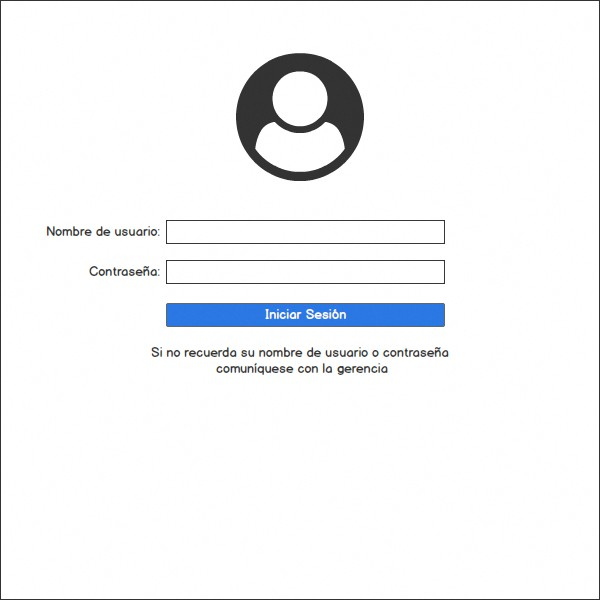
\includegraphics[scale = 0.5]{pantallas/us01_mockup.jpg}}%
	}%
	\caption*{Figura B.\arabic{counter_img_B}: Mock-up \hyperlink{US}{US} 1.}
	\addcontentsline{lof}{figure}{B.\arabic{counter_img_B}: Mock-up US 1.}
	\stepcounter{counter_img_B}
	\label{us01_mockup}
\end{figure}

\begin{figure}[H] 
	\centering
	\subfloat[Escritorio \hyperlink{US}{US} 1.]{%
		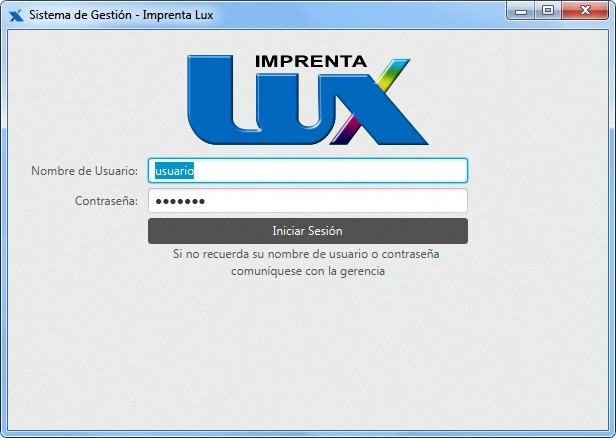
\includegraphics[width=0.73\textwidth]{pantallas/us01_desktop.jpg}%
		\label{fig:a}%
	}%
	\hfill%
	\subfloat[Móvil \hyperlink{US}{US} 1.]{%
		\setlength{\fboxrule}{0.5pt}%
		\fbox{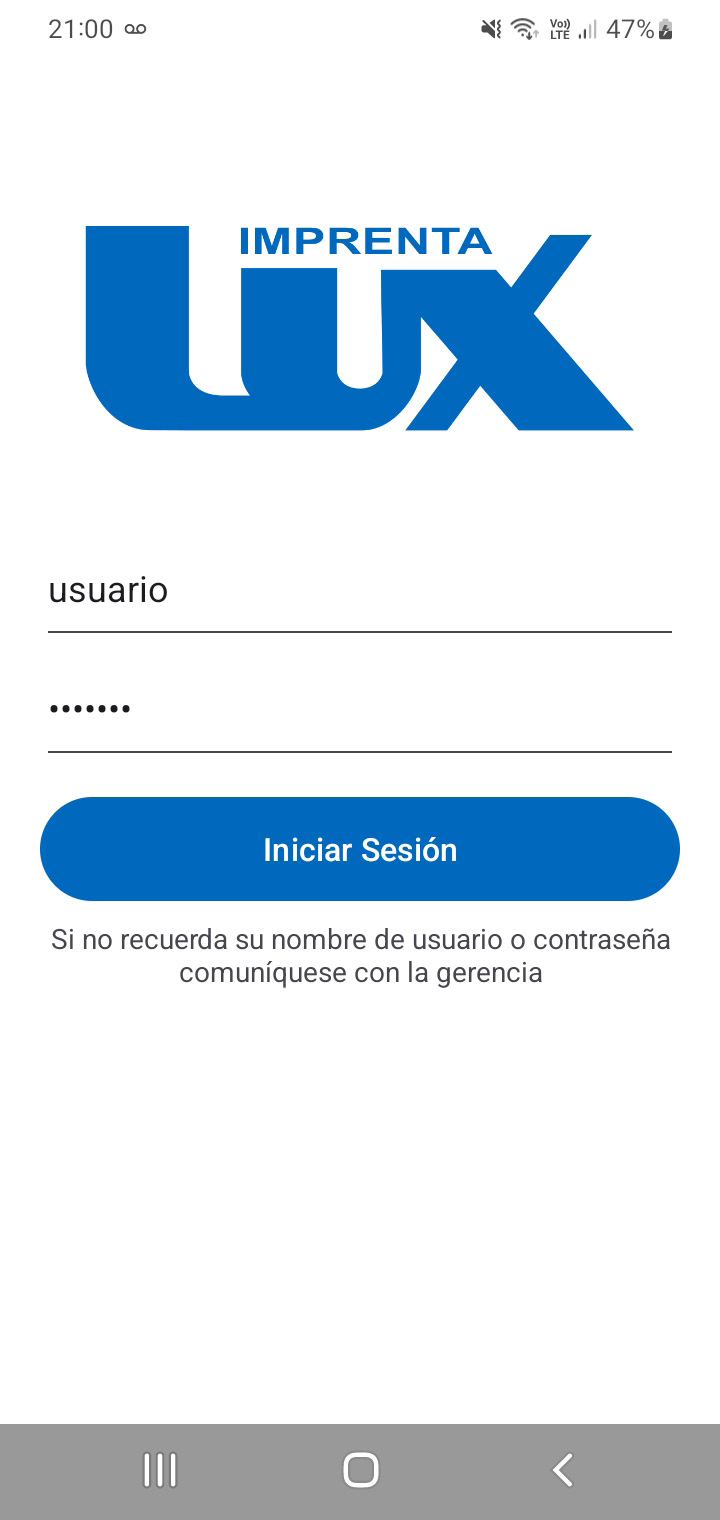
\includegraphics[width=0.24\textwidth]
			{pantallas/us01_mobile.jpg}}%
		\label{fig:b}%
	}%
	\caption*{Figura B.\arabic{counter_img_B}: Versiones de escritorio y móvil de pantalla correspondiente a \hyperlink{US}{US} 1.}
	\addcontentsline{lof}{figure}{B.\arabic{counter_img_B}: Versiones de escritorio y móvil de pantalla correspondiente a US 1.}
	\stepcounter{counter_img_B}
\end{figure}


\subsection*{Administrar usuarios (\hyperlink{US}{US} 2)}

\begin{figure}[H]
	\centering
	{%
		\setlength{\fboxsep}{0pt}%
		\setlength{\fboxrule}{0.5pt}%
		\fbox{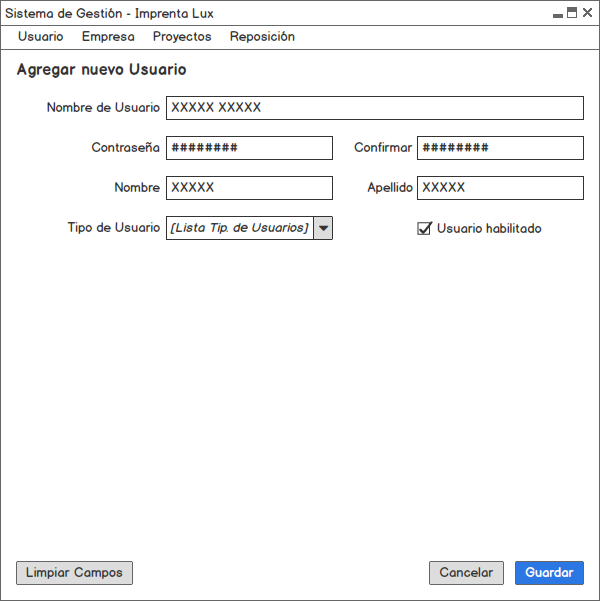
\includegraphics[scale = 0.47]{pantallas/us02_mockup_new.png}}%
	}%
	\caption*{Figura B.\arabic{counter_img_B}: Mock-up \hyperlink{US}{US} 2 (nuevo usuario).}
	\addcontentsline{lof}{figure}{B.\arabic{counter_img_B}: Mock-up US 2 (nuevo usuario).}
	\stepcounter{counter_img_B}
	\label{us02_mockup}
\end{figure}

\begin{figure}[H] 
	\centering
	\subfloat[Escritorio \hyperlink{US}{US} 2 (nuevo).]{%
		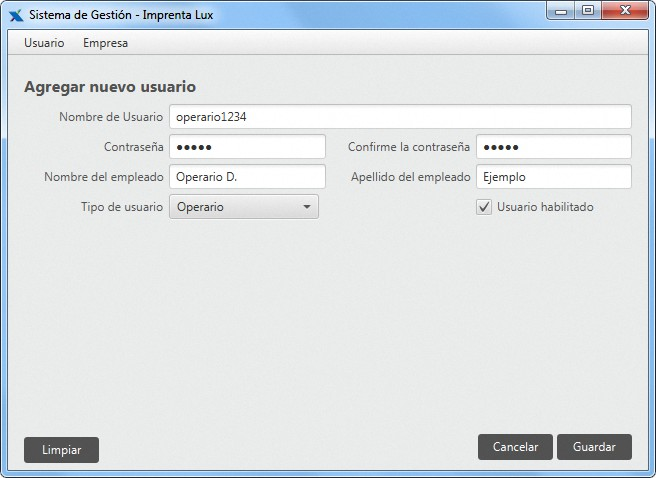
\includegraphics[width=0.73\textwidth]{pantallas/us02_desktop_new.jpg}%
		\label{fig:a}%
	}%
	\hfill%
	\subfloat[Móvil \hyperlink{US}{US} 2 (nuevo).]{%
		\setlength{\fboxrule}{0.5pt}%
		\fbox{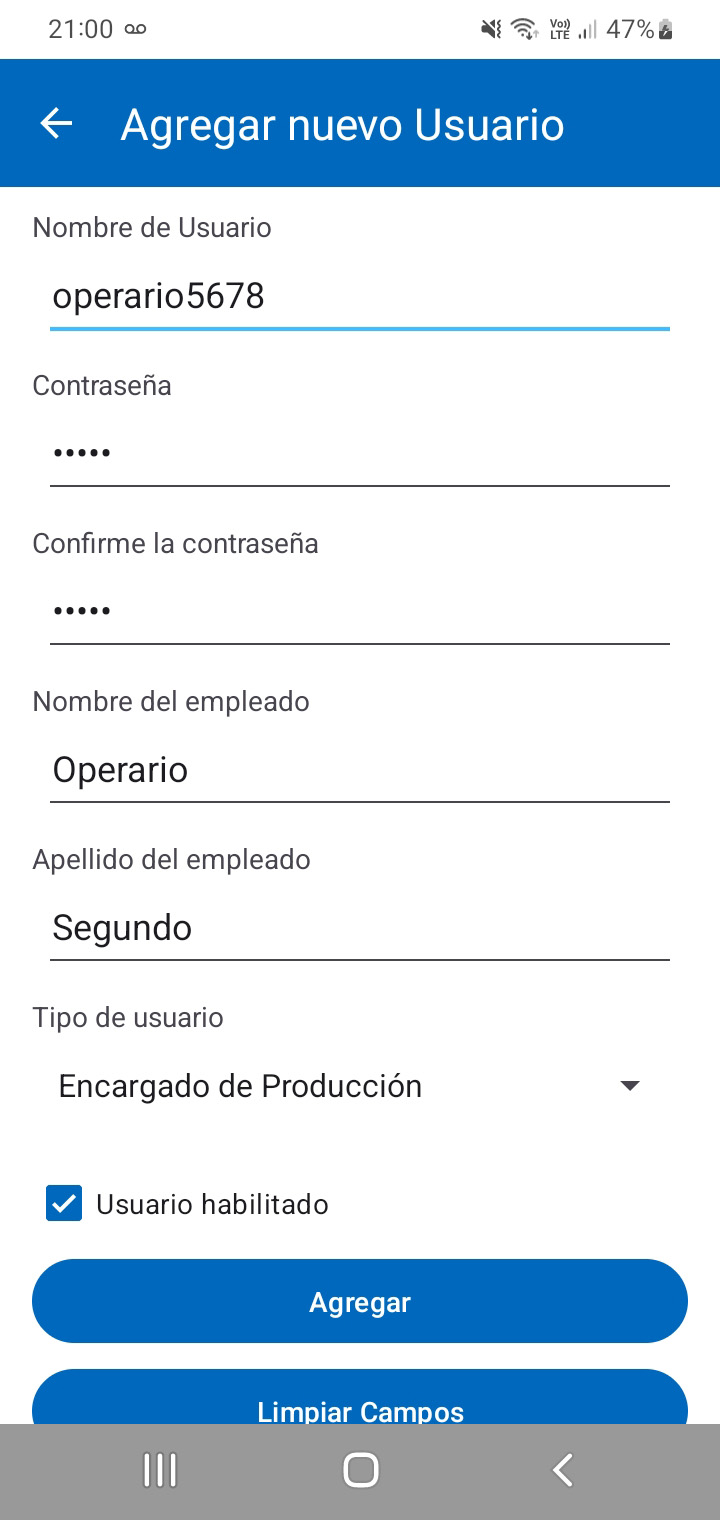
\includegraphics[width=0.24\textwidth]
			{pantallas/us02_mobile_new.jpg}}%
		\label{fig:b}%
	}%
	\caption*{Figura B.\arabic{counter_img_B}: Versiones de escritorio y móvil de pantalla correspondiente a \hyperlink{US}{US} 2 (nuevo usuario).}
	\addcontentsline{lof}{figure}{B.\arabic{counter_img_B}: Versiones de escritorio y móvil de pantalla correspondiente a US 2 (nuevo usuario).}
	\stepcounter{counter_img_B}
\end{figure}

\begin{figure}[H]
	\centering
	{%
		\setlength{\fboxsep}{0pt}%
		\setlength{\fboxrule}{0.5pt}%
		\fbox{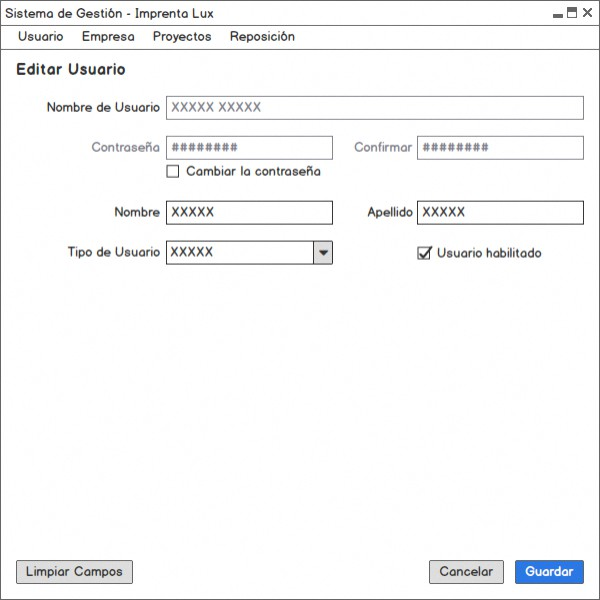
\includegraphics[scale = 0.47]{pantallas/us02_mockup_edit.jpg}}%
	}%
	\caption*{Figura B.\arabic{counter_img_B}: Mock-up \hyperlink{US}{US} 2 (editar usuario).}
	\addcontentsline{lof}{figure}{B.\arabic{counter_img_B}: Mock-up US 2 (editar usuario).}
	\stepcounter{counter_img_B}
	\label{us02_mockup_edit}
\end{figure}

\begin{figure}[H] 
	\centering
	\subfloat[Escritorio \hyperlink{US}{US} 2 (editar).]{%
		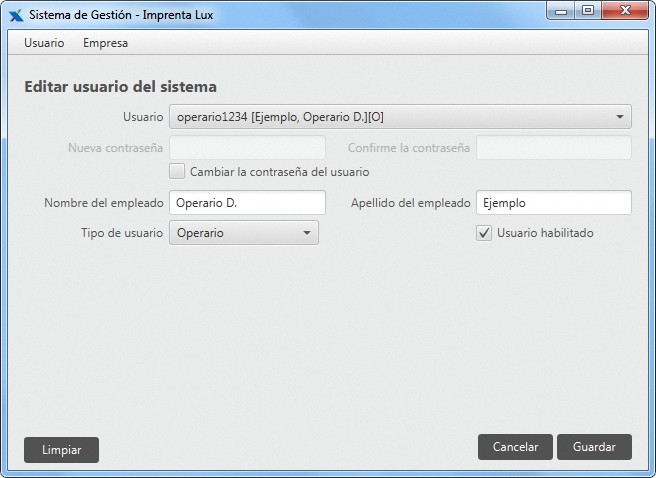
\includegraphics[width=0.73\textwidth]{pantallas/us02_desktop_edit.jpg}%
		\label{fig:a}%
	}%
	\hfill%
	\subfloat[Móvil \hyperlink{US}{US} 2 (editar).]{%
		\setlength{\fboxrule}{0.5pt}%
		\fbox{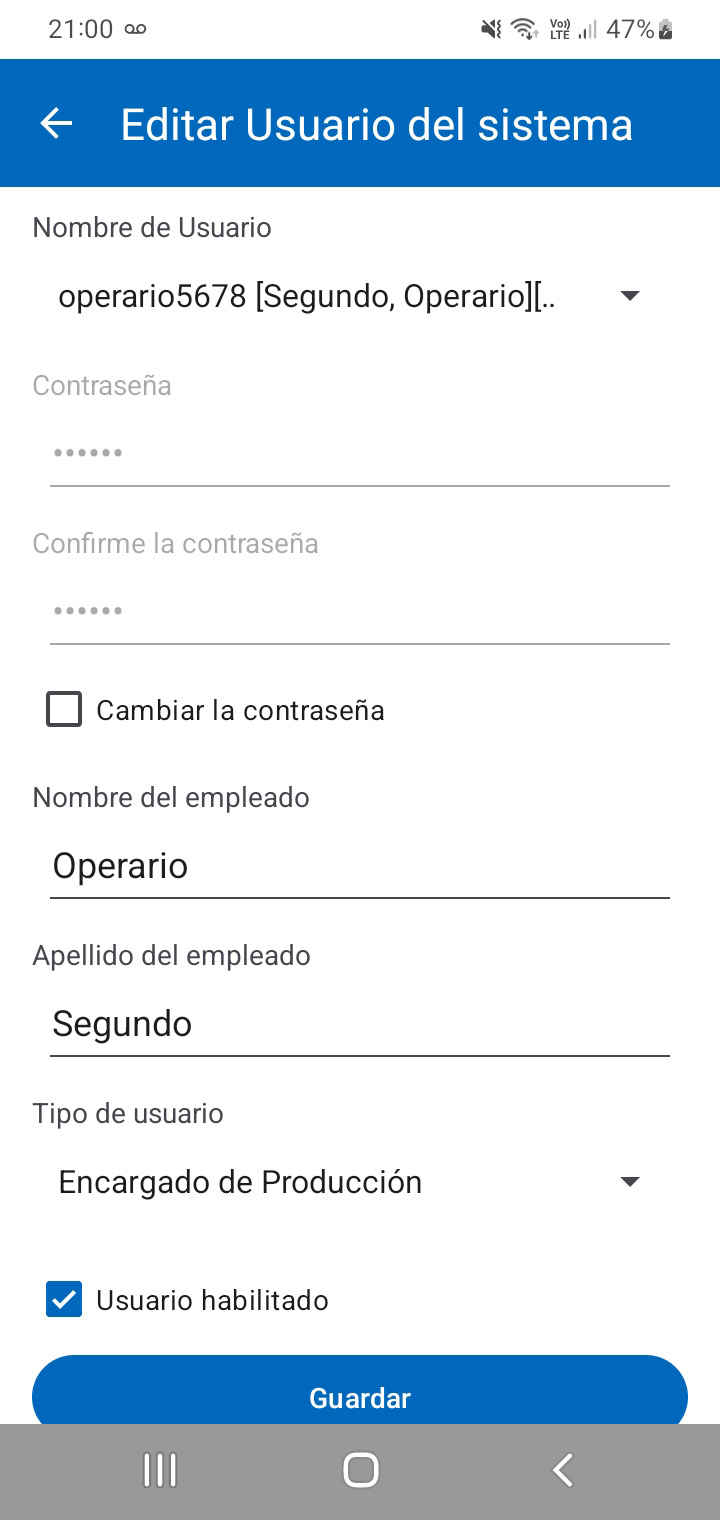
\includegraphics[width=0.24\textwidth]
			{pantallas/us02_mobile_edit.jpg}}%
		\label{fig:b}%
	}%
	\caption*{Figura B.\arabic{counter_img_B}: Versiones de escritorio y móvil de pantalla correspondiente a \hyperlink{US}{US} 2  (editar usuario).}
	\addcontentsline{lof}{figure}{B.\arabic{counter_img_B}: Versiones de escritorio y móvil de pantalla correspondiente a US 2 (editar usuario).}
	\stepcounter{counter_img_B}
\end{figure}


\subsection*{Administrar depósitos (\hyperlink{US}{US} 6)}

\begin{figure}[H]
	\centering
	{%
		\setlength{\fboxsep}{0pt}%
		\setlength{\fboxrule}{0.5pt}%
		\fbox{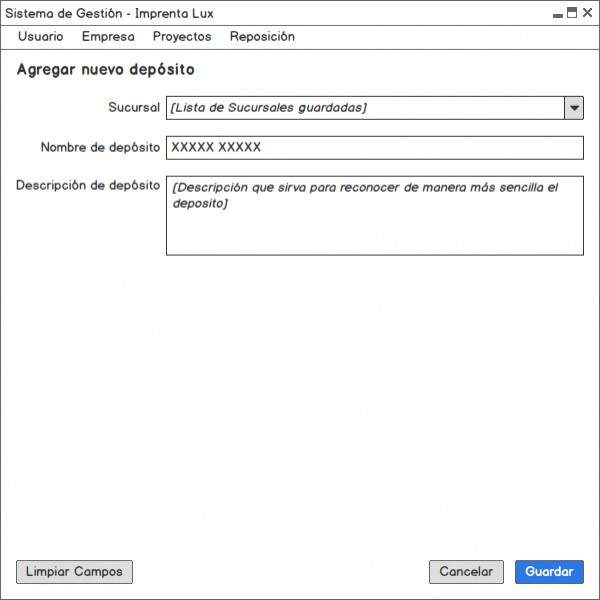
\includegraphics[scale = 0.47]{pantallas/us06_mockup_new.jpg}}%
	}%
	\caption*{Figura B.\arabic{counter_img_B}: Mock-up \hyperlink{US}{US} 6 (nuevo depósito).}
	\addcontentsline{lof}{figure}{B.\arabic{counter_img_B}: Mock-up US 6 (nuevo depósito).}
	\stepcounter{counter_img_B}
	\label{us06_mockup}
\end{figure}

\begin{figure}[H] 
	\centering
	\subfloat[Escritorio \hyperlink{US}{US} 6 (nuevo).]{%
		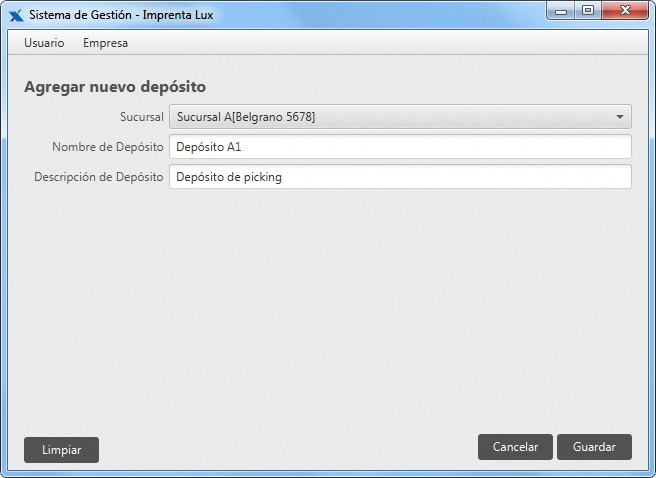
\includegraphics[width=0.73\textwidth]{pantallas/us06_desktop_new.jpg}%
		\label{fig:a}%
	}%
	\hfill%
	\subfloat[Móvil \hyperlink{US}{US} 6 (nuevo).]{%
		\setlength{\fboxrule}{0.5pt}%
		\fbox{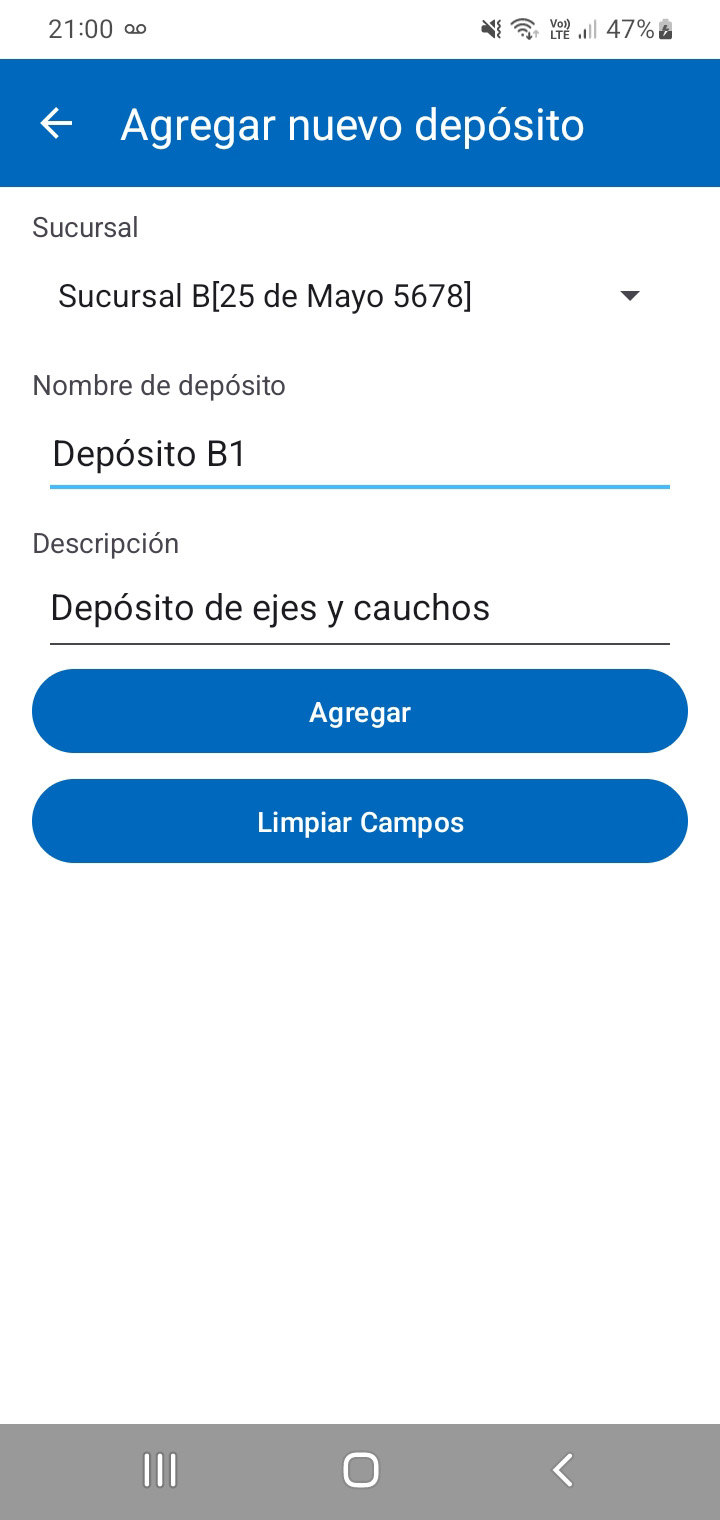
\includegraphics[width=0.24\textwidth]
			{pantallas/us06_mobile_new.jpg}}%
		\label{fig:b}%
	}%
	\caption*{Figura B.\arabic{counter_img_B}: Versiones de escritorio y móvil de pantalla correspondiente a \hyperlink{US}{US} 6  (nuevo depósito).}
	\addcontentsline{lof}{figure}{B.\arabic{counter_img_B}: Versiones de escritorio y móvil de pantalla correspondiente a US 6 (nuevo depósito).}
	\stepcounter{counter_img_B}
\end{figure}

\begin{figure}[H]
	\centering
	{%
		\setlength{\fboxsep}{0pt}%
		\setlength{\fboxrule}{0.5pt}%
		\fbox{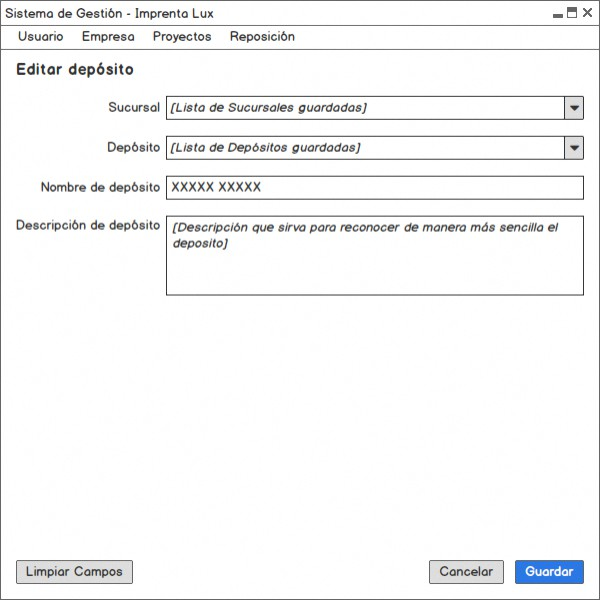
\includegraphics[scale = 0.47]{pantallas/us06_mockup_edit.jpg}}%
	}%
	\caption*{Figura B.\arabic{counter_img_B}: Mock-up \hyperlink{US}{US} 6 (editar depósito).}
	\addcontentsline{lof}{figure}{B.\arabic{counter_img_B}: Mock-up US 6 (editar depósito).}
	\stepcounter{counter_img_B}
	\label{us06_mockup_edit}
\end{figure}

\begin{figure}[H] 
	\centering
	\subfloat[Escritorio \hyperlink{US}{US} 6 (editar).]{%
		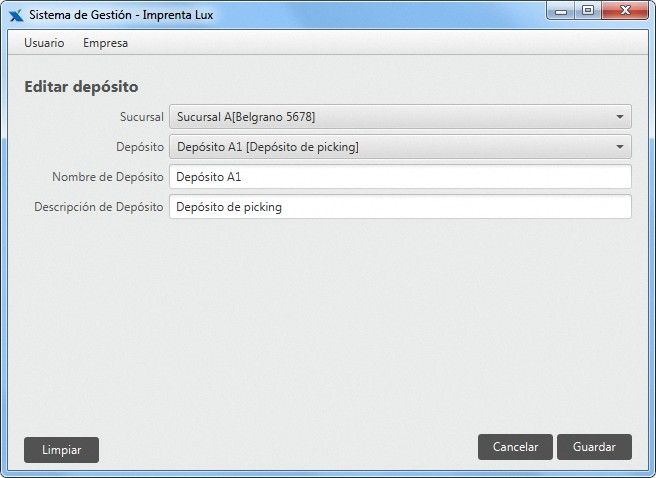
\includegraphics[width=0.73\textwidth]{pantallas/us06_desktop_edit.jpg}%
		\label{fig:a}%
	}%
	\hfill%
	\subfloat[Móvil \hyperlink{US}{US} 6 (editar).]{%
		\setlength{\fboxrule}{0.5pt}%
		\fbox{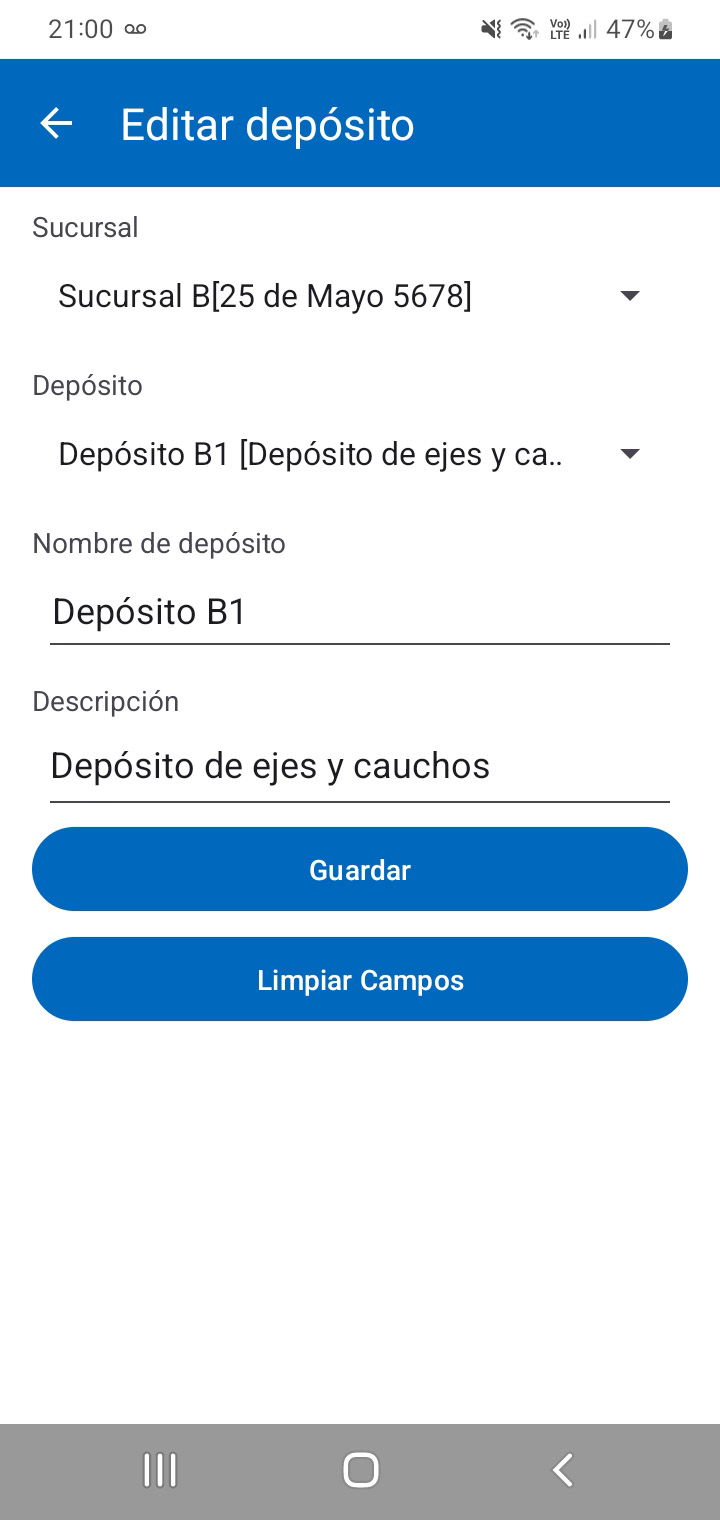
\includegraphics[width=0.24\textwidth]
			{pantallas/us06_mobile_edit.jpg}}%
		\label{fig:b}%
	}%
	\caption*{Figura B.\arabic{counter_img_B}: Versiones de escritorio y móvil de pantalla correspondiente a \hyperlink{US}{US} 6  (editar depósito).}
	\addcontentsline{lof}{figure}{B.\arabic{counter_img_B}: Versiones de escritorio y móvil de pantalla correspondiente a US 6 (editar depósito).}
	\stepcounter{counter_img_B}
\end{figure}


\subsection*{Administrar sucursales (\hyperlink{US}{US} 7)}

\begin{figure}[H]
	\centering
	{%
		\setlength{\fboxsep}{0pt}%
		\setlength{\fboxrule}{0.5pt}%
		\fbox{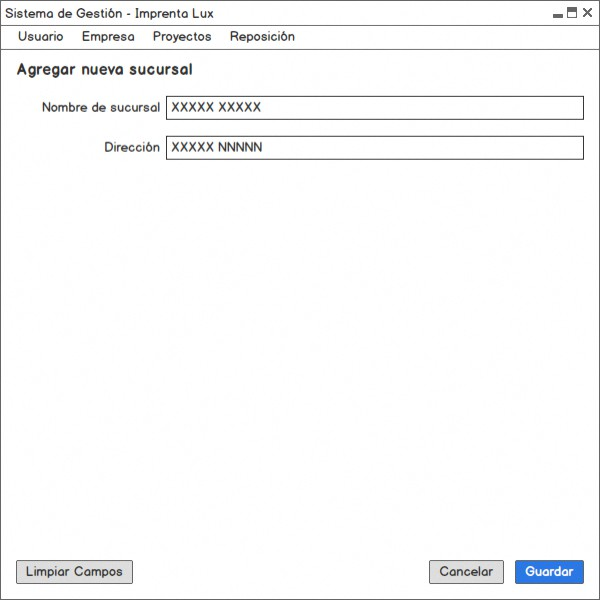
\includegraphics[scale = 0.47]{pantallas/us07_mockup_new.jpg}}%
	}%
	\caption*{Figura B.\arabic{counter_img_B}: Mock-up \hyperlink{US}{US} 7 (nueva sucursal).}
	\addcontentsline{lof}{figure}{B.\arabic{counter_img_B}: Mock-up US 7 (nueva sucursal).}
	\stepcounter{counter_img_B}
	\label{us07_mockup}
\end{figure}

\begin{figure}[H] 
	\centering
	\subfloat[Escritorio \hyperlink{US}{US} 7 (nueva).]{%
		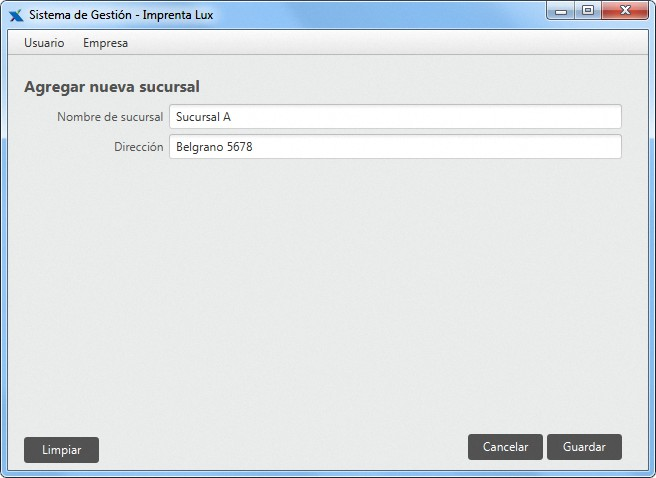
\includegraphics[width=0.73\textwidth]{pantallas/us07_desktop_new.jpg}%
		\label{fig:a}%
	}%
	\hfill%
	\subfloat[Móvil \hyperlink{US}{US} 7 (nueva).]{%
		\setlength{\fboxrule}{0.5pt}%
		\fbox{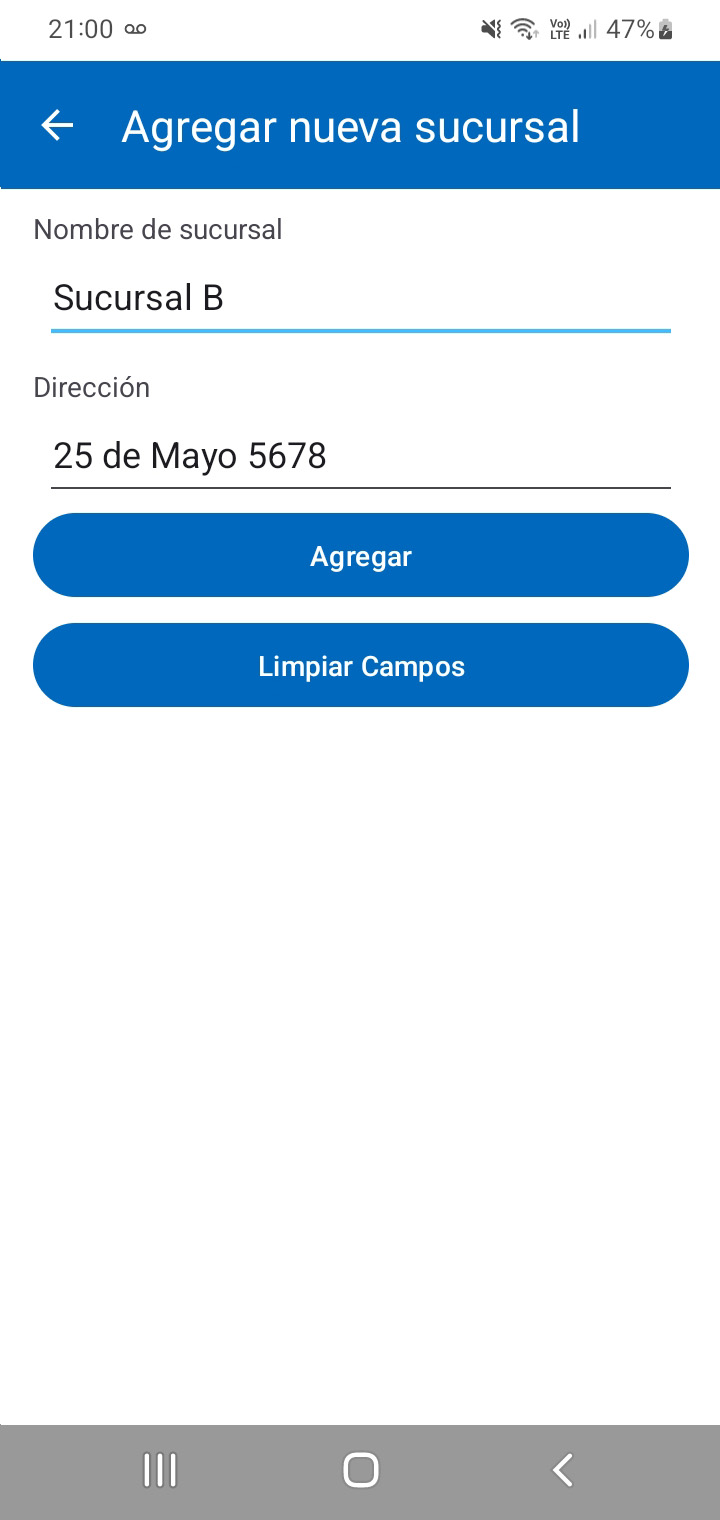
\includegraphics[width=0.24\textwidth]
			{pantallas/us07_mobile_new.jpg}}%
		\label{fig:b}%
	}%
	\caption*{Figura B.\arabic{counter_img_B}: Versiones de escritorio y móvil de pantalla correspondiente a \hyperlink{US}{US} 7  (nueva sucursal).}
	\addcontentsline{lof}{figure}{B.\arabic{counter_img_B}: Versiones de escritorio y móvil de pantalla correspondiente a US 7  (nueva sucursal).}
	\stepcounter{counter_img_B}
\end{figure}

\begin{figure}[H]
	\centering
	{%
		\setlength{\fboxsep}{0pt}%
		\setlength{\fboxrule}{0.5pt}%
		\fbox{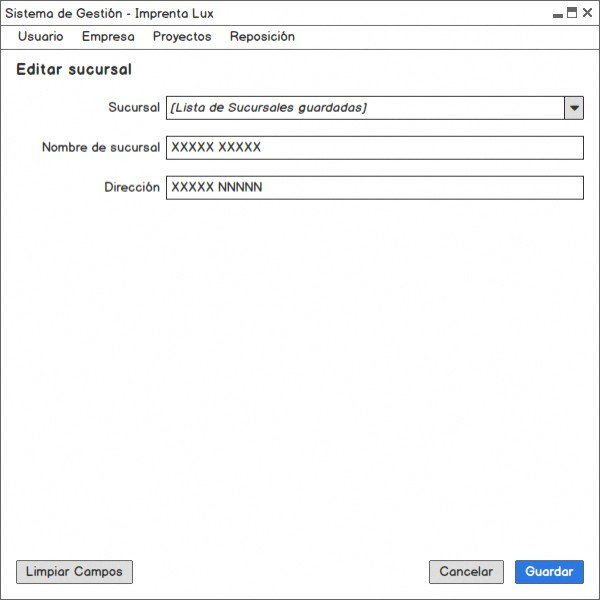
\includegraphics[scale = 0.47]{pantallas/us07_mockup_edit.jpg}}%
	}%
	\caption*{Figura B.\arabic{counter_img_B}: Mock-up \hyperlink{US}{US} 7 (editar sucursal).}
	\addcontentsline{lof}{figure}{B.\arabic{counter_img_B}: Mock-up US 7 (editar sucursal).}
	\stepcounter{counter_img_B}
	\label{us07_mockup_edit}
\end{figure}

\begin{figure}[H] 
	\centering
	\subfloat[Escritorio \hyperlink{US}{US} 7 (editar).]{%
		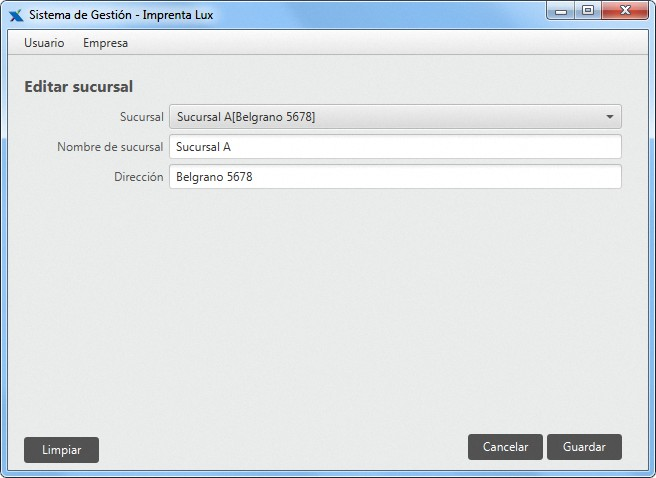
\includegraphics[width=0.73\textwidth]{pantallas/us07_desktop_edit.jpg}%
		\label{fig:a}%
	}%
	\hfill%
	\subfloat[Móvil \hyperlink{US}{US} 7 (editar).]{%
		\setlength{\fboxrule}{0.5pt}%
		\fbox{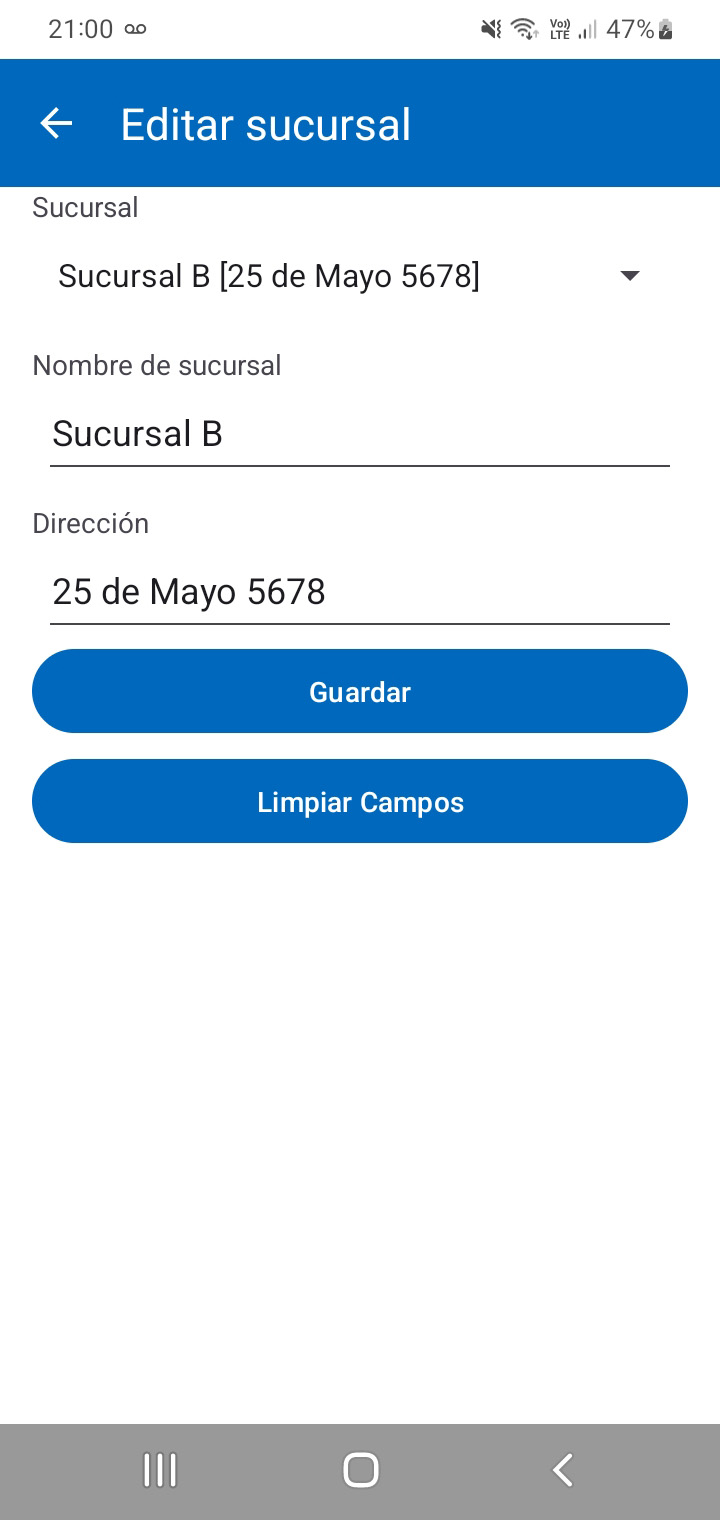
\includegraphics[width=0.24\textwidth]
			{pantallas/us07_mobile_edit.jpg}}%
		\label{fig:b}%
	}%
	\caption*{Figura B.\arabic{counter_img_B}: Versiones de escritorio y móvil de pantalla correspondiente a \hyperlink{US}{US} 7  (editar sucursal).}
	\addcontentsline{lof}{figure}{B.\arabic{counter_img_B}: Versiones de escritorio y móvil de pantalla correspondiente a US 7  (editar sucursal).}
	\stepcounter{counter_img_B}
\end{figure}


\subsection*{Administrar clientes (\hyperlink{US}{US} 18)}

\begin{figure}[H]
	\centering
	{%
		\setlength{\fboxsep}{0pt}%
		\setlength{\fboxrule}{0.5pt}%
		\fbox{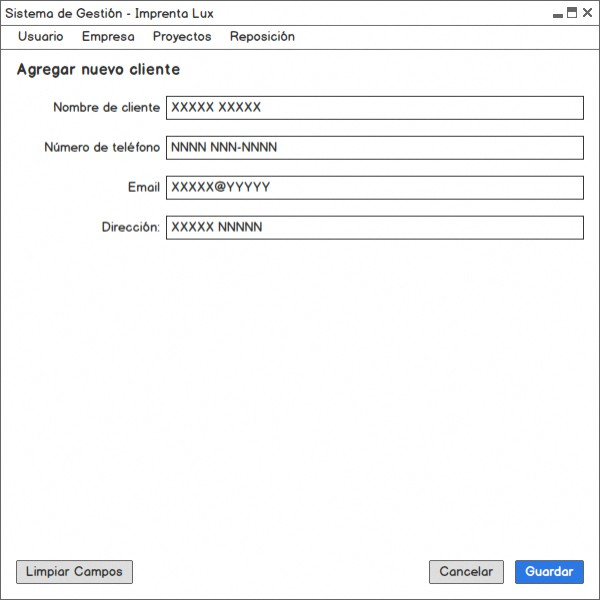
\includegraphics[scale = 0.47]{pantallas/us18_mockup_new.jpg}}%
	}%
	\caption*{Figura B.\arabic{counter_img_B}: Mock-up \hyperlink{US}{US} 18 (nuevo cliente).}
	\addcontentsline{lof}{figure}{B.\arabic{counter_img_B}: Mock-up US 18 (nuevo cliente).}
	\stepcounter{counter_img_B}
	\label{us18_mockup}
\end{figure}

\begin{figure}[H] 
	\centering
	\subfloat[Escritorio \hyperlink{US}{US} 18 (nuevo).]{%
		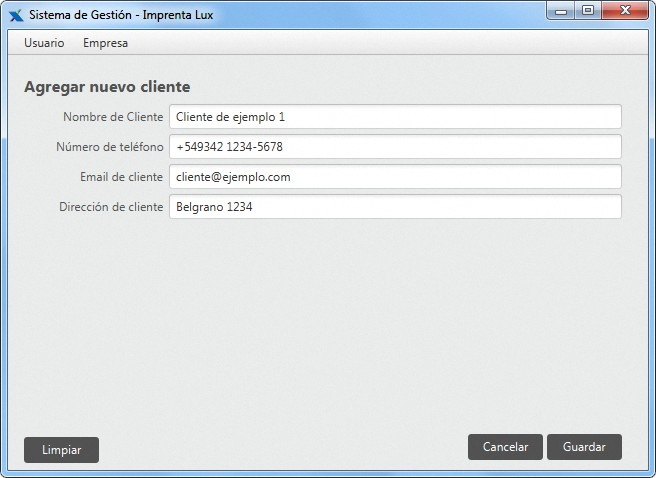
\includegraphics[width=0.73\textwidth]{pantallas/us18_desktop_new.jpg}%
		\label{fig:a}%
	}%
	\hfill%
	\subfloat[Móvil \hyperlink{US}{US} 18 (nuevo).]{%
		\setlength{\fboxrule}{0.45pt}%
		\fbox{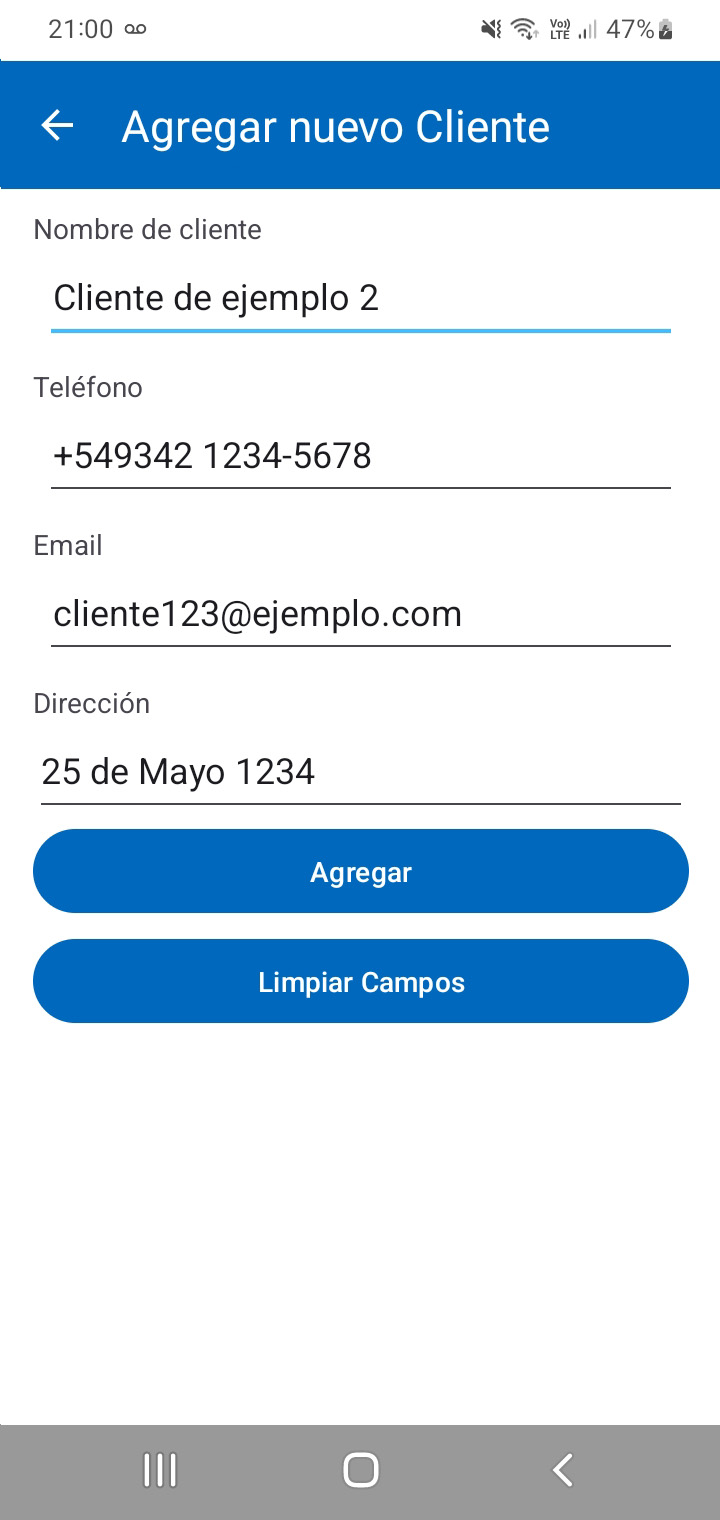
\includegraphics[width=0.24\textwidth]
			{pantallas/us18_mobile_new.jpg}}%
		\label{fig:b}%
	}%
	\caption*{Figura B.\arabic{counter_img_B}: Versiones de escritorio y móvil de pantalla correspondiente a \hyperlink{US}{US} 18  (nuevo cliente).}
	\addcontentsline{lof}{figure}{B.\arabic{counter_img_B}: Versiones de escritorio y móvil de pantalla correspondiente a US 18  (nuevo cliente).}
	\stepcounter{counter_img_B}
\end{figure}

\begin{figure}[H]
	\centering
	{%
		\setlength{\fboxsep}{0pt}%
		\setlength{\fboxrule}{0.5pt}%
		\fbox{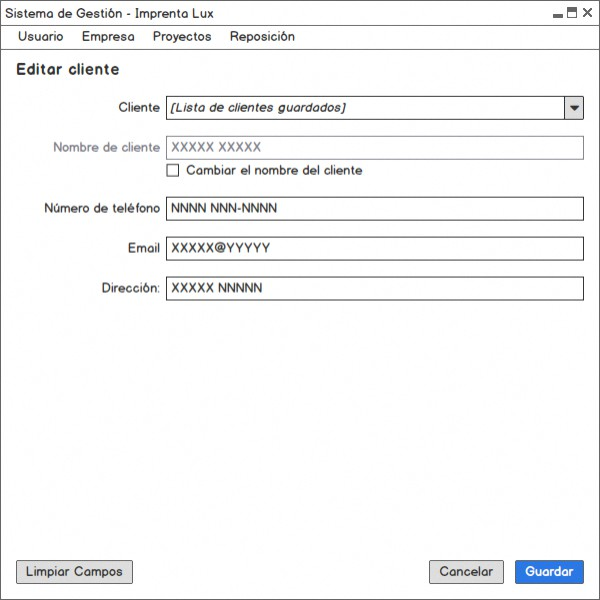
\includegraphics[scale = 0.47]{pantallas/us18_mockup_edit.jpg}}%
	}%
	\caption*{Figura B.\arabic{counter_img_B}: Mock-up \hyperlink{US}{US} 18 (editar cliente).}
	\addcontentsline{lof}{figure}{B.\arabic{counter_img_B}: Mock-up US 18 (editar cliente).}
	\stepcounter{counter_img_B}
	\label{us18_mockup_edit}
\end{figure}

\begin{figure}[H] 
	\centering
	\subfloat[Escritorio \hyperlink{US}{US} 18 (editar).]{%
		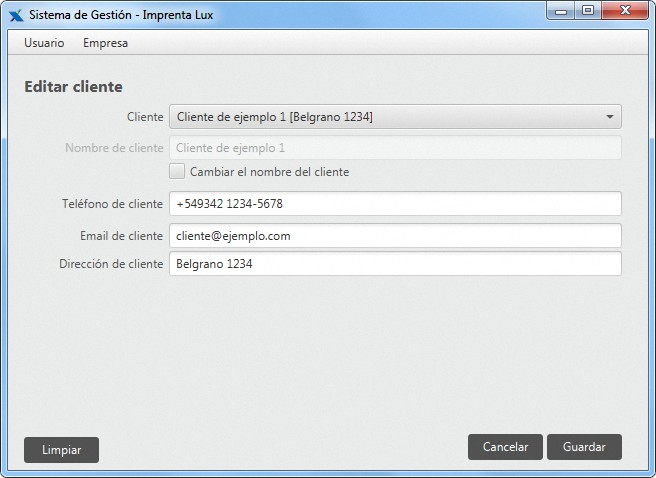
\includegraphics[width=0.73\textwidth]{pantallas/us18_desktop_edit.jpg}%
		\label{fig:a}%
	}%
	\hfill%
	\subfloat[Móvil \hyperlink{US}{US} 18 (editar).]{%
		\setlength{\fboxrule}{0.5pt}%
		\fbox{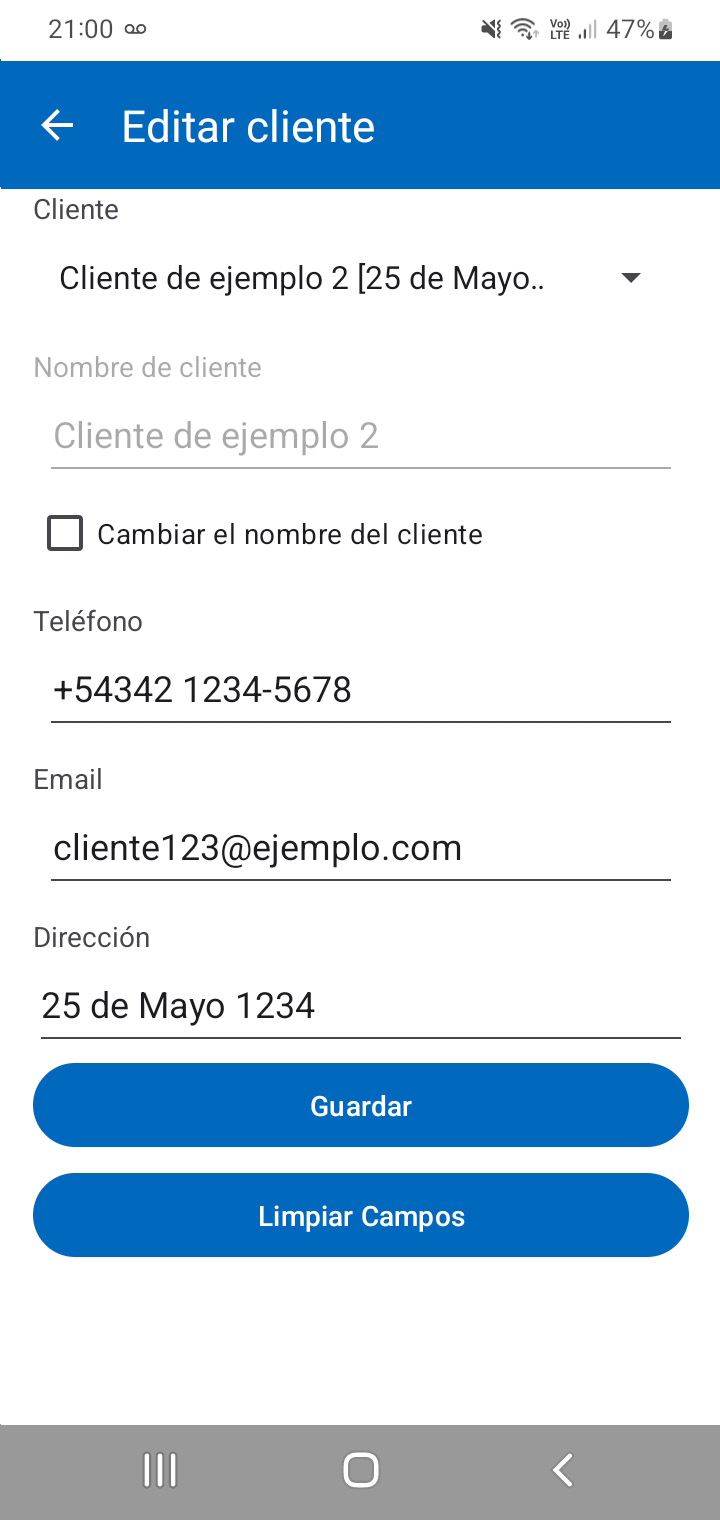
\includegraphics[width=0.24\textwidth]
			{pantallas/us18_mobile_edit.jpg}}%
		\label{fig:b}%
	}%
	\caption*{Figura B.\arabic{counter_img_B}: Versiones de escritorio y móvil de pantalla correspondiente a \hyperlink{US}{US} 18  (editar cliente).}
	\addcontentsline{lof}{figure}{B.\arabic{counter_img_B}: Versiones de escritorio y móvil de pantalla correspondiente a US 18  (editar cliente).}
	\stepcounter{counter_img_B}
\end{figure}
\pagebreak

\section*{Iteración II}

\subsection*{Administrar insumo (\hyperlink{US}{US} 3)}

\begin{figure}[H]
	\centering
	{%
		\setlength{\fboxsep}{0pt}%
		\setlength{\fboxrule}{0.5pt}%
		\fbox{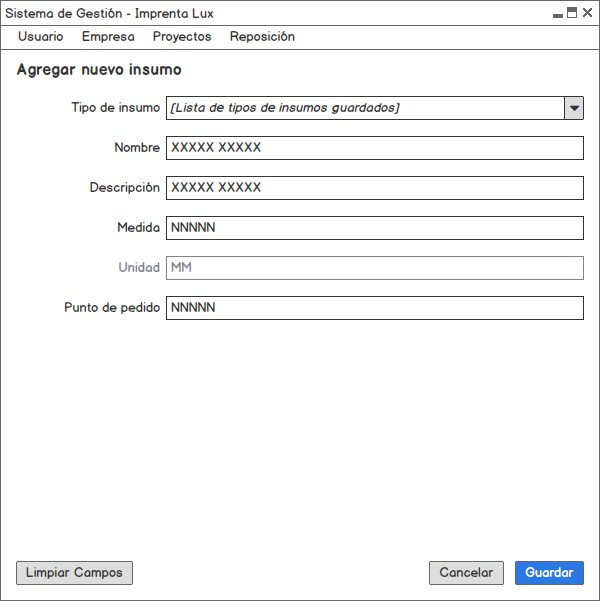
\includegraphics[scale = 0.4]{pantallas/us03_mockup_new.jpg}}%
	}%
	\caption*{Figura B.\arabic{counter_img_B}: Mock-up \hyperlink{US}{US} 3 (nuevo insumo).}
	\addcontentsline{lof}{figure}{B.\arabic{counter_img_B}: Mock-up US 3 (nuevo insumo).}
	\stepcounter{counter_img_B}
	\label{us01_mockup_new}
\end{figure}
\indent

\begin{figure}[H] 
	\centering
	\subfloat[Escritorio \hyperlink{US}{US} 3 (nuevo).]{%
		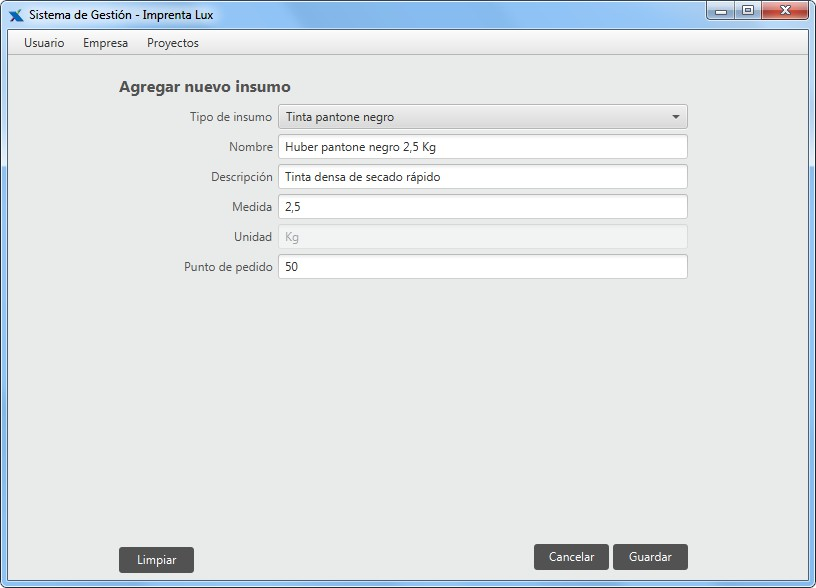
\includegraphics[width=0.73\textwidth]{pantallas/us03_desktop_new.jpg}%
		\label{fig:a}%
	}%
	\hfill%
	\subfloat[Móvil \hyperlink{US}{US} 3 (nuevo).]{%
		\setlength{\fboxrule}{0.5pt}%
		\fbox{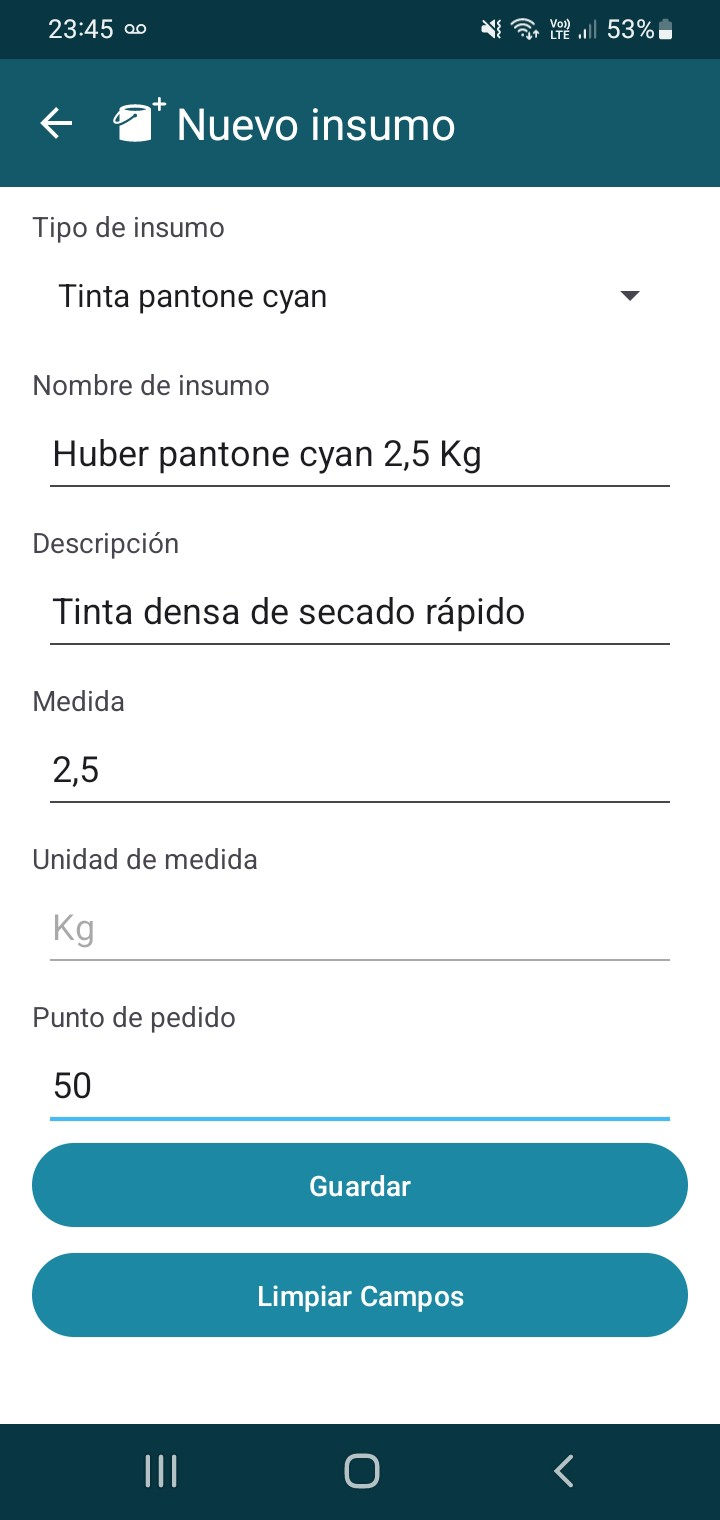
\includegraphics[width=0.24\textwidth]
			{pantallas/us03_mobile_new.jpg}}%
		\label{fig:b}%
	}%
	\caption*{Figura B.\arabic{counter_img_B}: Versiones de escritorio y móvil de pantalla correspondiente a \hyperlink{US}{US} 3 (nuevo insumo).}
	\addcontentsline{lof}{figure}{B.\arabic{counter_img_B}: Versiones de escritorio y móvil de pantalla correspondiente a US 3 (nuevo insumo).}
	\stepcounter{counter_img_B}
\end{figure}

\begin{figure}[H]
	\centering
	{%
		\setlength{\fboxsep}{0pt}%
		\setlength{\fboxrule}{0.5pt}%
		\fbox{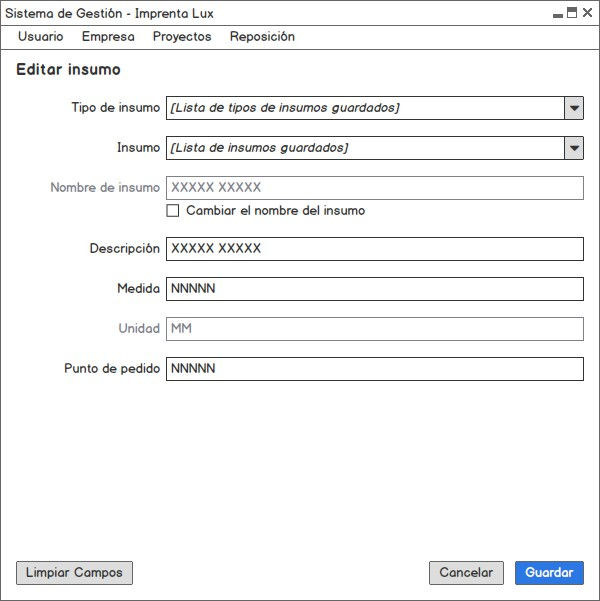
\includegraphics[scale = 0.5]{pantallas/us03_mockup_edit.jpg}}%
	}%
	\caption*{Figura B.\arabic{counter_img_B}: Mock-up \hyperlink{US}{US} 3 (editar insumo).}
	\addcontentsline{lof}{figure}{B.\arabic{counter_img_B}: Mock-up US 3 (editar insumo).}
	\stepcounter{counter_img_B}
	\label{us01_mockup}
\end{figure}

\begin{figure}[H] 
	\centering
	\subfloat[Escritorio \hyperlink{US}{US} 3 (editar).]{%
		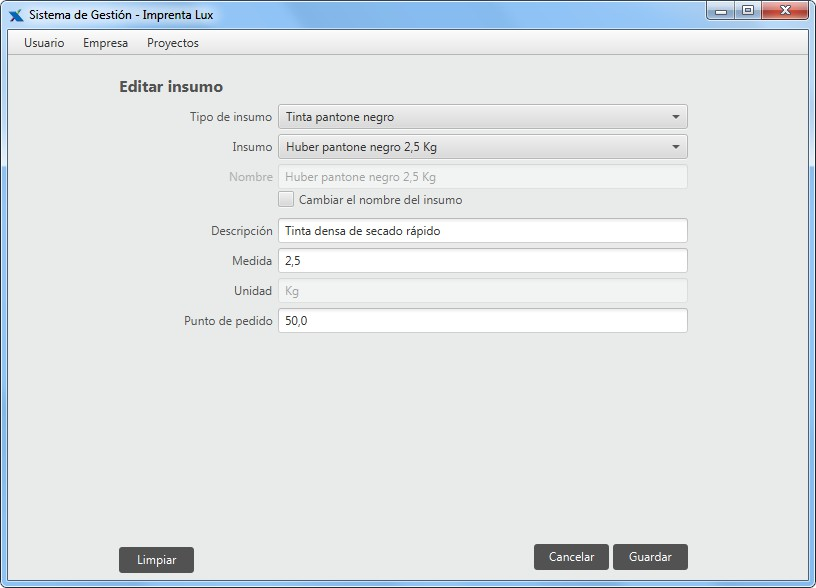
\includegraphics[width=0.73\textwidth]{pantallas/us03_desktop_edit.jpg}%
		\label{fig:a}%
	}%
	\hfill%
	\subfloat[Móvil \hyperlink{US}{US} 3 (editar).]{%
		\setlength{\fboxrule}{0.5pt}%
		\fbox{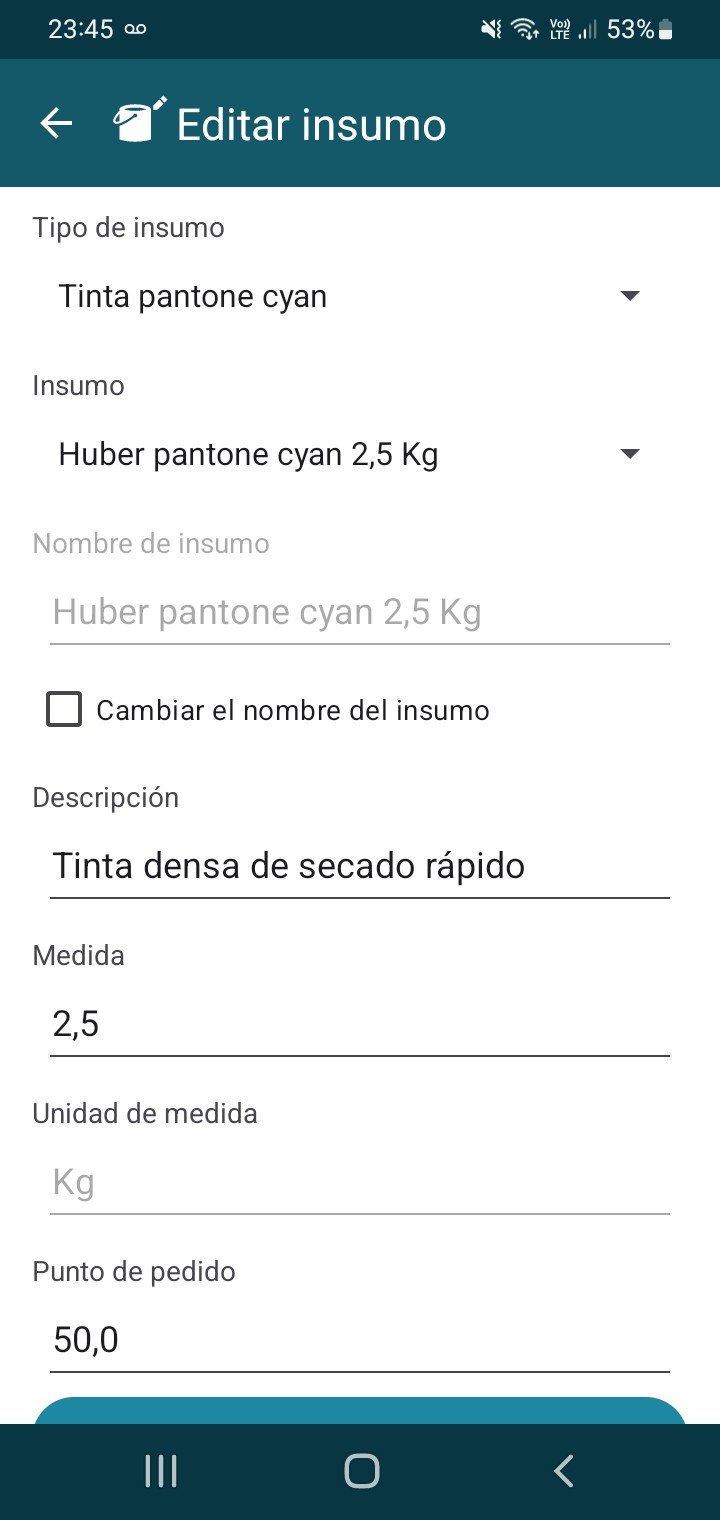
\includegraphics[width=0.24\textwidth]
			{pantallas/us03_mobile_edit.jpg}}%
		\label{fig:b}%
	}%
	\caption*{Figura B.\arabic{counter_img_B}: Versiones de escritorio y móvil de pantalla correspondiente a \hyperlink{US}{US} 3 (editar insumo).}
	\addcontentsline{lof}{figure}{B.\arabic{counter_img_B}: Versiones de escritorio y móvil de pantalla correspondiente a US 3 (editar insumo).}
	\stepcounter{counter_img_B}
\end{figure}


\subsection*{Administrar tipo de insumo (\hyperlink{US}{US} 4)}

\begin{figure}[H]
	\centering
	{%
		\setlength{\fboxsep}{0pt}%
		\setlength{\fboxrule}{0.5pt}%
		\fbox{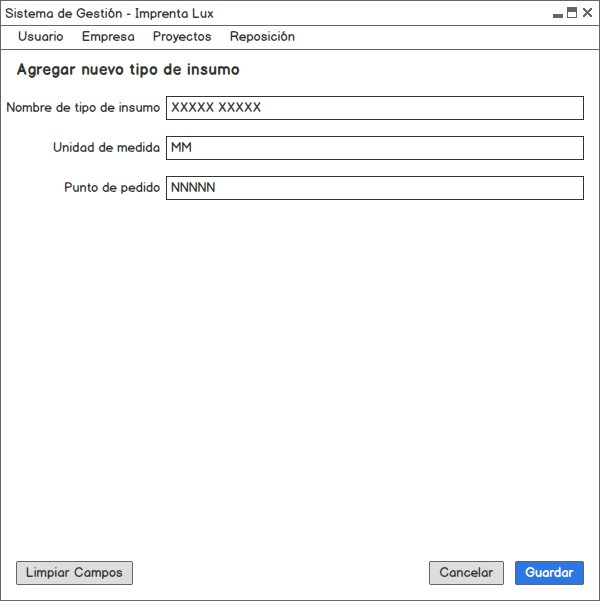
\includegraphics[scale = 0.43]{pantallas/us04_mockup_new.jpg}}%
	}%
	\caption*{Figura B.\arabic{counter_img_B}: Mock-up \hyperlink{US}{US} 4 (nuevo tipo de insumo).}
	\addcontentsline{lof}{figure}{B.\arabic{counter_img_B}: Mock-up US 4 (nuevo tipo de insumo).}
	\stepcounter{counter_img_B}
	\label{us04_mockup}
\end{figure}

\begin{figure}[H] 
	\centering
	\subfloat[Escritorio \hyperlink{US}{US} 4 (nuevo).]{%
		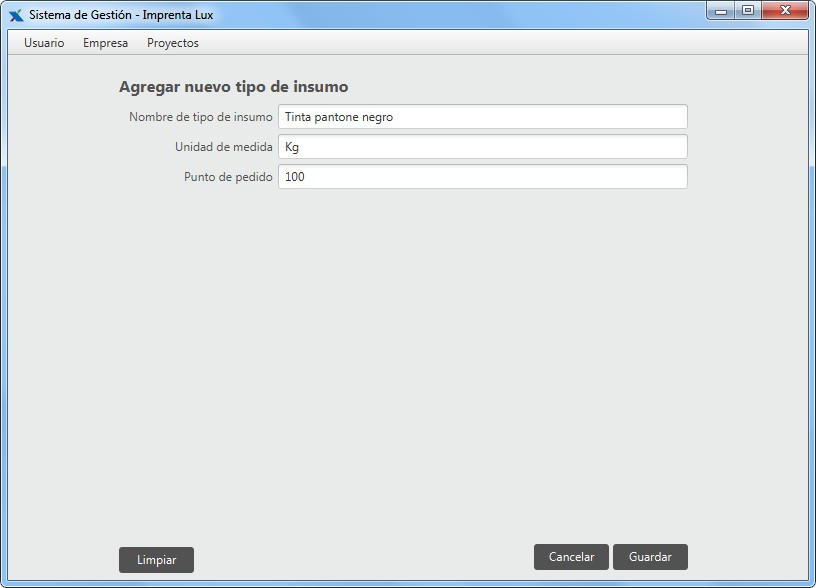
\includegraphics[width=0.73\textwidth]{pantallas/us04_desktop_new.jpg}%
		\label{fig:a}%
	}%
	\hfill%
	\subfloat[Móvil \hyperlink{US}{US} 4 (nuevo).]{%
		\setlength{\fboxrule}{0.5pt}%
		\fbox{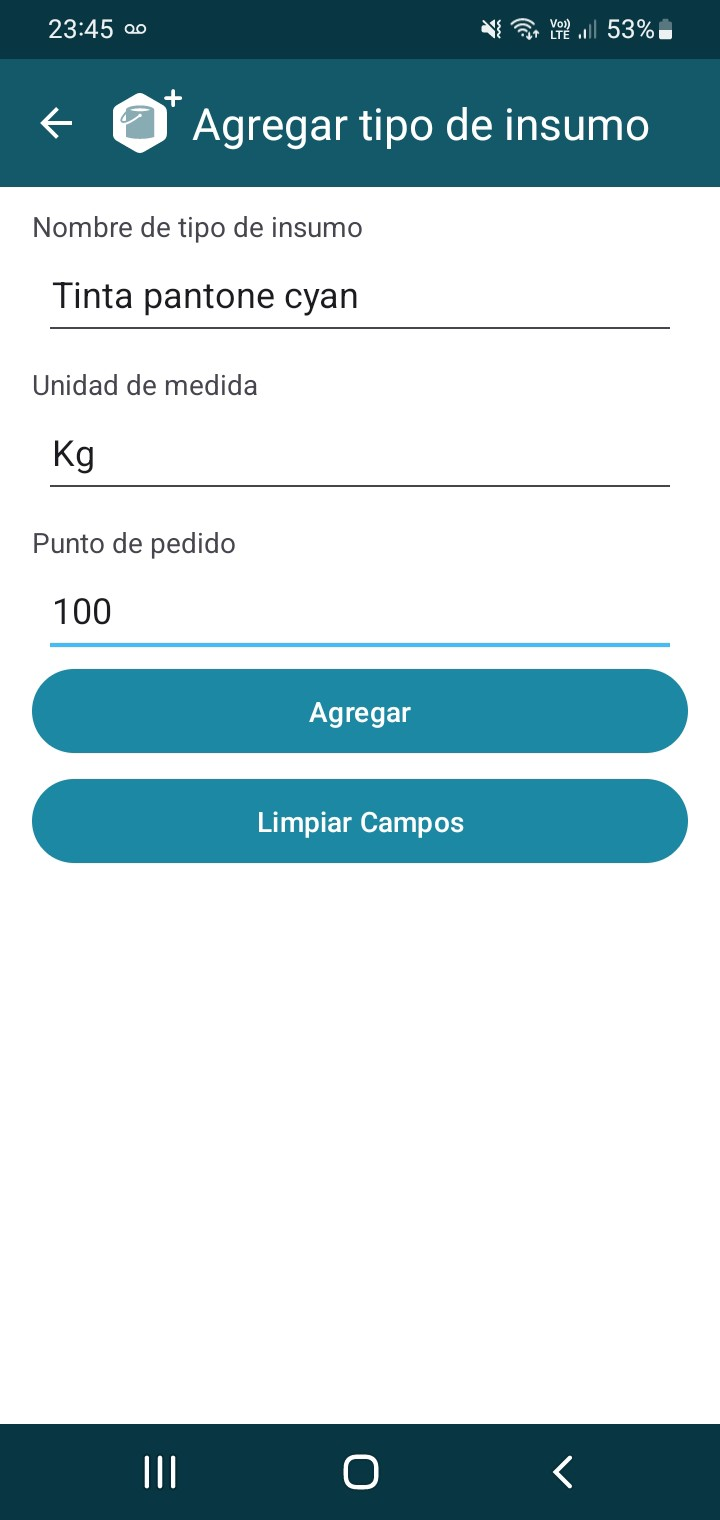
\includegraphics[width=0.24\textwidth]
			{pantallas/us04_mobile_new.jpg}}%
		\label{fig:b}%
	}%
	\caption*{Figura B.\arabic{counter_img_B}: Versiones de escritorio y móvil de pantalla correspondiente a \hyperlink{US}{US} 4  (nuevo tipo de insumo).}
	\addcontentsline{lof}{figure}{B.\arabic{counter_img_B}: Versiones de escritorio y móvil de pantalla correspondiente a US 4  (nuevo tipo de insumo).}
	\stepcounter{counter_img_B}
\end{figure}

\begin{figure}[H]
	\centering
	{%
		\setlength{\fboxsep}{0pt}%
		\setlength{\fboxrule}{0.5pt}%
		\fbox{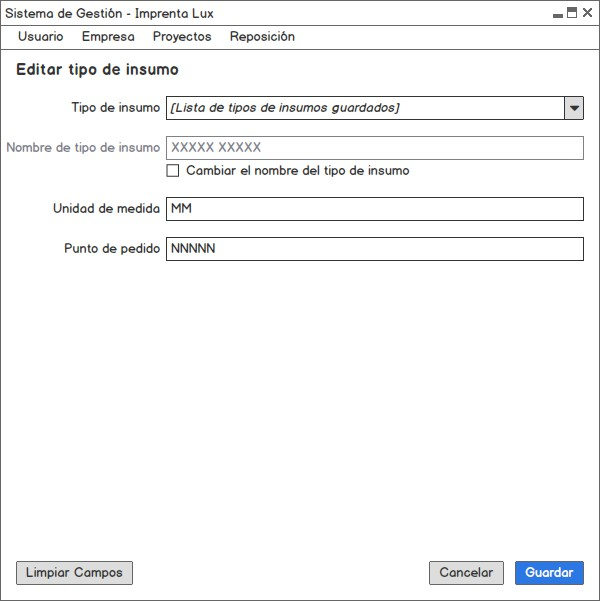
\includegraphics[scale = 0.47]{pantallas/us04_mockup_edit.jpg}}%
	}%
	\caption*{Figura B.\arabic{counter_img_B}: Mock-up \hyperlink{US}{US} 4 (editar tipo de insumo).}
	\addcontentsline{lof}{figure}{B.\arabic{counter_img_B}: Mock-up US 4 (editar tipo de insumo).}
	\stepcounter{counter_img_B}
	\label{us04_mockup_edit}
\end{figure}

\begin{figure}[H] 
	\centering
	\subfloat[Escritorio \hyperlink{US}{US} 4 (editar).]{%
		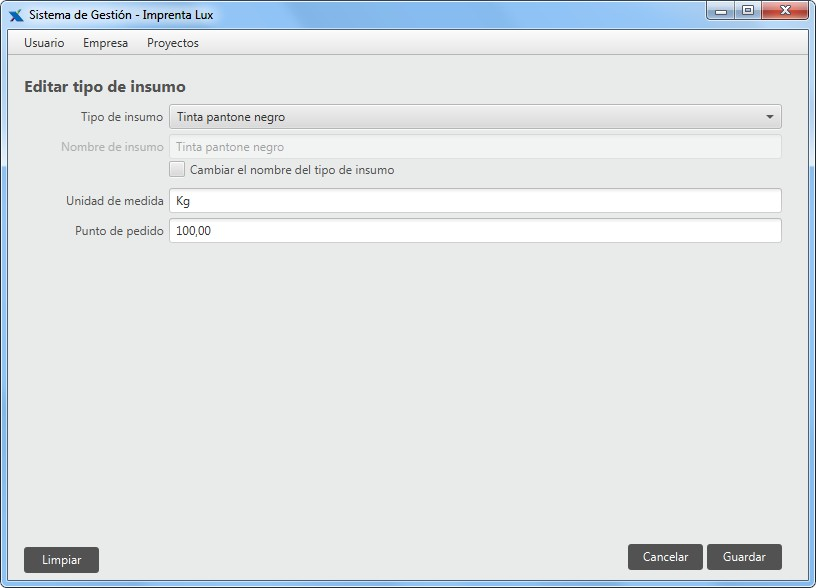
\includegraphics[width=0.73\textwidth]{pantallas/us04_desktop_edit.jpg}%
		\label{fig:a}%
	}%
	\hfill%
	\subfloat[Móvil \hyperlink{US}{US} 4 (editar).]{%
		\setlength{\fboxrule}{0.5pt}%
		\fbox{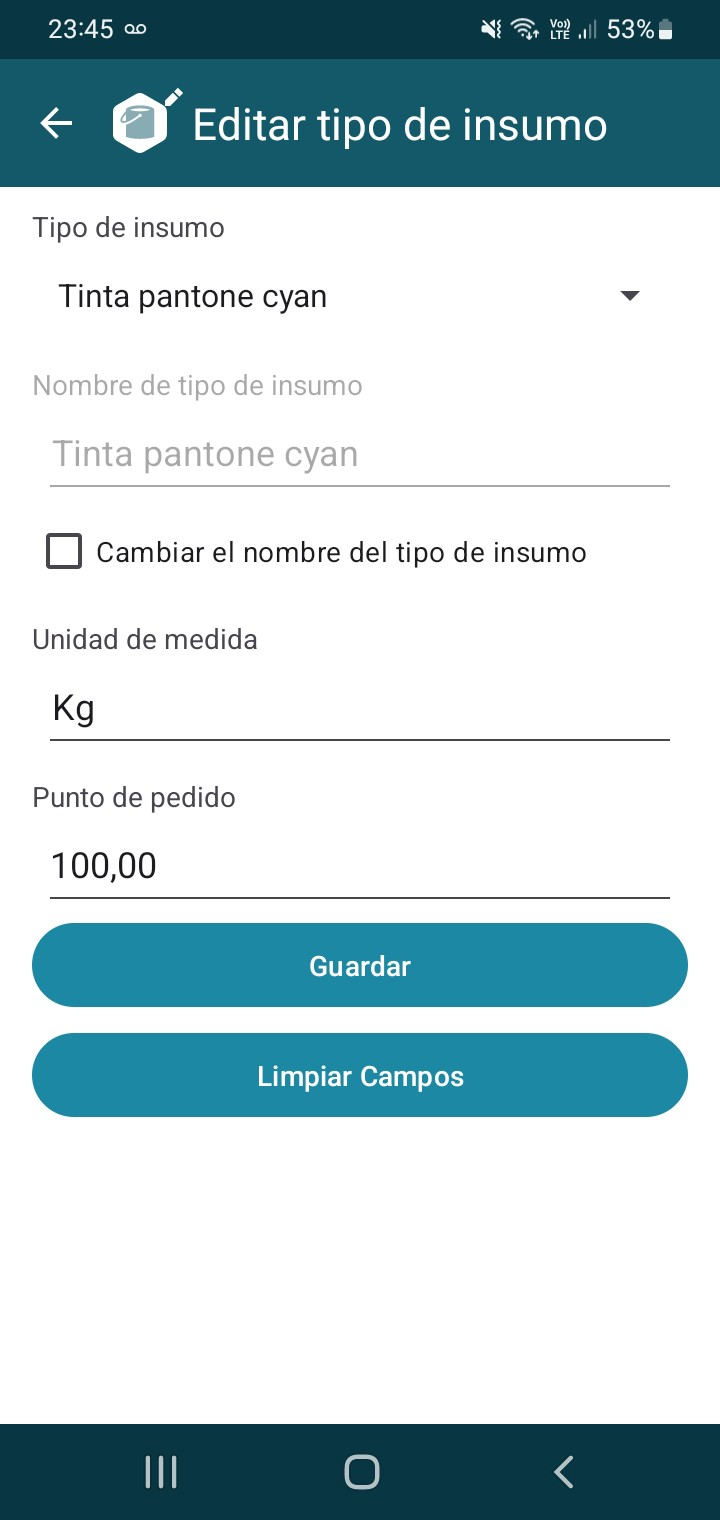
\includegraphics[width=0.24\textwidth]
			{pantallas/us04_mobile_edit.jpg}}%
		\label{fig:b}%
	}%
	\caption*{Figura B.\arabic{counter_img_B}: Versiones de escritorio y móvil de pantalla correspondiente a \hyperlink{US}{US} 4  (editar tipo de insumo).}
	\addcontentsline{lof}{figure}{B.\arabic{counter_img_B}: Versiones de escritorio y móvil de pantalla correspondiente a US 4  (editar tipo de insumo).}
	\stepcounter{counter_img_B}
\end{figure}


\subsection*{Modificar cantidad de insumo (\hyperlink{US}{US} 5)}

\begin{figure}[H]
	\centering
	{%
		\setlength{\fboxsep}{0pt}%
		\setlength{\fboxrule}{0.5pt}%
		\fbox{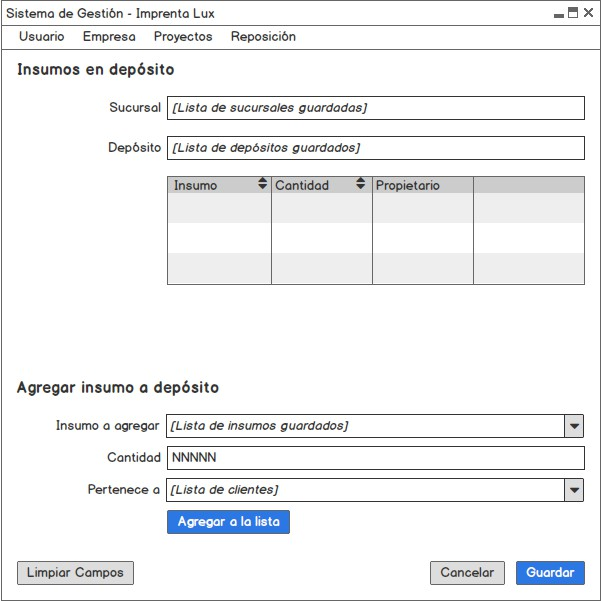
\includegraphics[scale = 0.45]{pantallas/us05_mockup_new.jpg}}%
	}%
	\caption*{Figura B.\arabic{counter_img_B}: Mock-up \hyperlink{US}{US} 5 (nuevo insumo en depósito).}
	\addcontentsline{lof}{figure}{B.\arabic{counter_img_B}: Mock-up US 5 (nuevo insumo en depósito).}
	\stepcounter{counter_img_B}
	\label{us05_mockup}
\end{figure}

\begin{figure}[H] 
	\centering
	\subfloat[Escritorio \hyperlink{US}{US} 5 (nuevo).]{%
		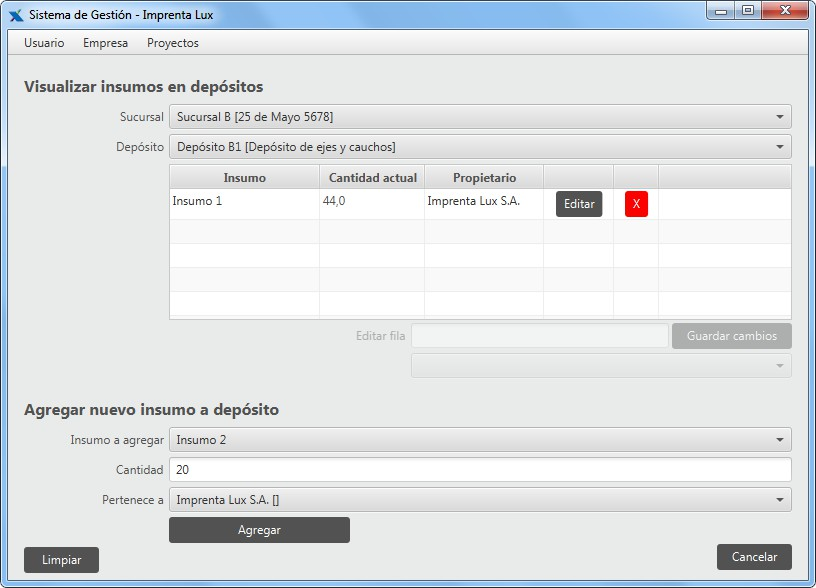
\includegraphics[width=0.73\textwidth]{pantallas/us05_desktop_new.jpg}%
		\label{fig:a}%
	}%
	\hfill%
	\subfloat[Móvil \hyperlink{US}{US} 5 (nuevo).]{%
		\setlength{\fboxrule}{0.5pt}%
		\fbox{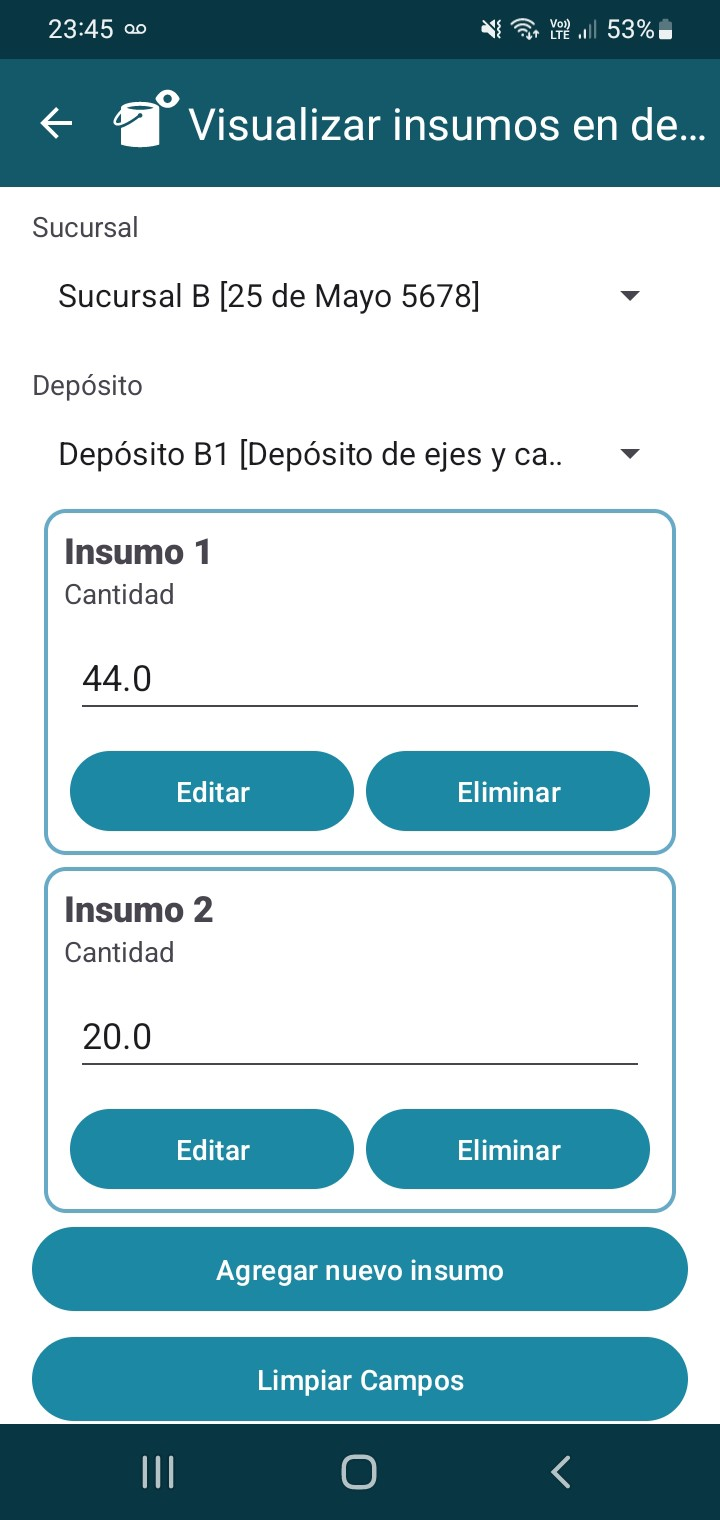
\includegraphics[width=0.24\textwidth]
			{pantallas/us05_mobile_new.jpg}}%
		\label{fig:b}%
	}%
	\caption*{Figura B.\arabic{counter_img_B}: Versiones de escritorio y móvil de pantalla correspondiente a \hyperlink{US}{US} 5  (nuevo insumo en depósito).}
	\addcontentsline{lof}{figure}{B.\arabic{counter_img_B}: Versiones de escritorio y móvil de pantalla correspondiente a US 5  (nuevo insumo en depósito).}
	\stepcounter{counter_img_B}
\end{figure}

\begin{figure}[H]
	\centering
	{%
		\setlength{\fboxsep}{0pt}%
		\setlength{\fboxrule}{0.5pt}%
		\fbox{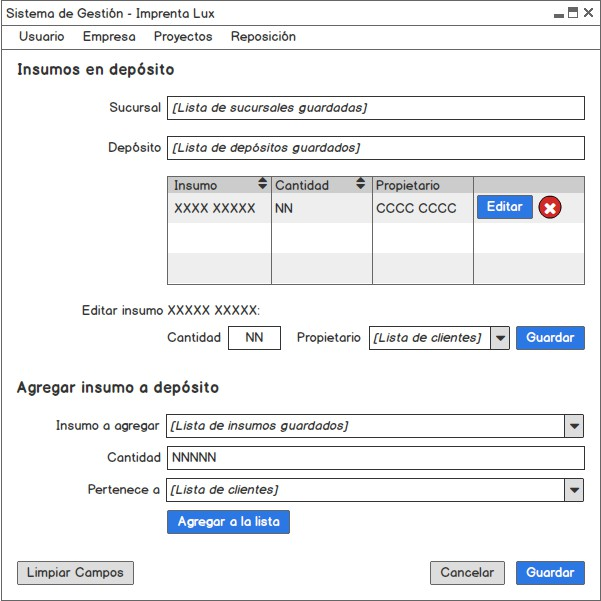
\includegraphics[scale = 0.47]{pantallas/us05_mockup_edit.jpg}}%
	}%
	\caption*{Figura B.\arabic{counter_img_B}: Mock-up \hyperlink{US}{US} 5 (editar cantidad de insumo en depósito).}
	\addcontentsline{lof}{figure}{B.\arabic{counter_img_B}: Mock-up US 5 (editar cantidad de insumo en depósito).}
	\stepcounter{counter_img_B}
	\label{us05_mockup_edit}
\end{figure}

\begin{figure}[H]
	\centering
	{\includegraphics[scale = 0.65]{pantallas/us05_desktop_edit.jpg}%
	}%
	\caption*{Figura B.\arabic{counter_img_B}: Versión de escritorio de pantalla correspondiente a \hyperlink{US}{US} 5  (editar cantidad de insumo en depósito).}
	\addcontentsline{lof}{figure}{B.\arabic{counter_img_B}: Versión de escritorio de pantalla correspondiente a US 5  (editar cantidad de insumo en depósito).}
	\stepcounter{counter_img_B}
	\label{us23_mockup_new}
\end{figure}


\subsection*{Administrar tipo de tarea (\hyperlink{US}{US} 23)}

\begin{figure}[H]
	\centering
	{%
		\setlength{\fboxsep}{0pt}%
		\setlength{\fboxrule}{0.5pt}%
		\fbox{\includegraphics[scale = 0.45]{pantallas/us23_mockup_new.jpg}}%
	}%
	\caption*{Figura B.\arabic{counter_img_B}: Mock-up \hyperlink{US}{US} 23 (nuevo tipo de tarea).}
	\addcontentsline{lof}{figure}{B.\arabic{counter_img_B}: Mock-up US 23 (nuevo tipo de tarea).}
	\stepcounter{counter_img_B}
	\label{us23_mockup_new}
\end{figure}

\begin{figure}[H]
	\centering
	{\includegraphics[scale = 0.60]{pantallas/us23_desktop_new.jpg}%
	}%
	\caption*{Figura B.\arabic{counter_img_B}: Versión de escritorio de pantalla correspondiente a \hyperlink{US}{US} 23  (nuevo tipo de tarea).}
	\addcontentsline{lof}{figure}{B.\arabic{counter_img_B}: Versión de escritorio de pantalla correspondiente a US 23  (nuevo tipo de tarea).}
	\stepcounter{counter_img_B}
	\label{us23_mockup}
\end{figure}

\begin{figure}[H]
	\centering
	{%
		\setlength{\fboxsep}{0pt}%
		\setlength{\fboxrule}{0.5pt}%
		\fbox{\includegraphics[scale = 0.47]{pantallas/us23_mockup_list.jpg}}%
	}%
	\caption*{Figura B.\arabic{counter_img_B}: Mock-up \hyperlink{US}{US} 23 (lista de tipos de tarea).}
	\addcontentsline{lof}{figure}{B.\arabic{counter_img_B}: Mock-up US 23 (lista de tipos de tarea).}
	\stepcounter{counter_img_B}
	\label{us23_mockup}
\end{figure}

\begin{figure}[H] 
	\centering
	\subfloat[Escritorio \hyperlink{US}{US} 23 (lista).]{%
		\includegraphics[width=0.73\textwidth]{pantallas/us23_desktop_list.jpg}%
		\label{fig:a}%
	}%
	\hfill%
	\subfloat[Móvil \hyperlink{US}{US} 23 (lista).]{%
		\setlength{\fboxrule}{0.5pt}%
		\fbox{\includegraphics[width=0.24\textwidth]
			{pantallas/us23_mobile_list.jpg}}%
		\label{fig:b}%
	}%
	\caption*{Figura B.\arabic{counter_img_B}: Versiones de escritorio y móvil de pantalla correspondiente a \hyperlink{US}{US} 23  (lista de tipos de tarea).}
	\addcontentsline{lof}{figure}{B.\arabic{counter_img_B}: Versiones de escritorio y móvil de pantalla correspondiente a US 23  (lista de tipos de tarea).}
	\stepcounter{counter_img_B}
\end{figure}

\begin{figure}[H] 
	\centering
	\subfloat[Móvil \hyperlink{US}{US} 23 (editar 1).]{%
		\setlength{\fboxrule}{0.5pt}%
		\fbox{\includegraphics[width=0.24\textwidth]
			{pantallas/us23_mobile_edit_1.jpg}}%
		\label{fig:b}%
	}%
	\hspace{0.5cm}%
	\subfloat[Móvil \hyperlink{US}{US} 23 (editar 2).]{%
		\setlength{\fboxrule}{0.5pt}%
		\fbox{\includegraphics[width=0.24\textwidth]
			{pantallas/us23_mobile_edit_2.jpg}}%
		\label{fig:b}%
	}%
	\caption*{Figura B.\arabic{counter_img_B}: Versión móvil de pantalla correspondiente a \hyperlink{US}{US} 23  (editar tipo de tarea).}
	\addcontentsline{lof}{figure}{B.\arabic{counter_img_B}: Versión móvil de pantalla correspondiente a US 23  (editar tipo de tarea).}
	\stepcounter{counter_img_B}
\end{figure}

\subsection*{Visualizar novedades (\hyperlink{US}{US} 24)}

\begin{figure}[H]
	\centering
	{%
		\setlength{\fboxsep}{0pt}%
		\setlength{\fboxrule}{0.5pt}%
		\fbox{\includegraphics[scale = 0.47]{pantallas/us24_mockup_list.jpg}}%
	}%
	\caption*{Figura B.\arabic{counter_img_B}: Mock-up \hyperlink{US}{US} 24.}
	\addcontentsline{lof}{figure}{B.\arabic{counter_img_B}: Mock-up US 24.}
	\stepcounter{counter_img_B}
	\label{us24_mockup}
\end{figure}

\begin{figure}[H] 
	\centering
	\subfloat[Escritorio \hyperlink{US}{US} 24.]{%
		\includegraphics[width=0.73\textwidth]{pantallas/us24_desktop_list.jpg}%
		\label{fig:a}%
	}%
	\hfill%
	\subfloat[Móvil \hyperlink{US}{US} 24.]{%
		\setlength{\fboxrule}{0.45pt}%
		\fbox{\includegraphics[width=0.24\textwidth]
			{pantallas/us24_mobile_list.jpg}}%
		\label{fig:b}%
	}%
	\caption*{Figura B.\arabic{counter_img_B}: Versiones de escritorio y móvil de pantalla correspondiente a \hyperlink{US}{US} 24.}
	\addcontentsline{lof}{figure}{B.\arabic{counter_img_B}: Versiones de escritorio y móvil de pantalla correspondiente a US 24.}
	\stepcounter{counter_img_B}
\end{figure}


\section*{Iteración III}

\subsection*{Administrar proyecto (\hyperlink{US}{US} 8)}

\begin{figure}[H] 
	\centering
	\subfloat[Mock-up \hyperlink{US}{US} 8 (nuevo proyecto 1).]{%
		\setlength{\fboxsep}{0pt}%
		\setlength{\fboxrule}{0.5pt}%
		\fbox{\includegraphics[width=0.53\textwidth]{pantallas/us08_mockup_new_1.jpg}}%
		\label{fig:a}%
	}%
	\hfill%
	\subfloat[Mock-up \hyperlink{US}{US} 8 (nuevo proyecto 2).]{%
		\setlength{\fboxsep}{0pt}%
		\setlength{\fboxrule}{0.5pt}%
		\fbox{\includegraphics[width=0.53\textwidth]
			{pantallas/us08_mockup_new_2.jpg}}%
		\label{fig:b}%
	}%
	\caption*{Figura B.\arabic{counter_img_B}: Mock-ups correspondientes a \hyperlink{US}{US} 8 (nuevo proyecto).}
	\addcontentsline{lof}{figure}{B.\arabic{counter_img_B}: Mock-ups correspondientes a US 8 (nuevo proyecto).}
	\stepcounter{counter_img_B}
\end{figure}

\begin{figure}[H] 
	\centering
	\subfloat[Escritorio \hyperlink{US}{US} 8 (nuevo 1).]{%
		\includegraphics[width=0.73\textwidth]{pantallas/us08_desktop_new_1.jpg}%
		\label{fig:a}%
	}%
	\hfill%
	\subfloat[Escritorio \hyperlink{US}{US} 8 (nuevo 2).]{%
		\includegraphics[width=0.73\textwidth]
		{pantallas/us08_desktop_new_2.jpg}%
		\label{fig:b}%
	}%
	\caption*{Figura B.\arabic{counter_img_B}: Versión de escritorio de pantallas correspondientes a \hyperlink{US}{US} 8 (nuevo proyecto).}
	\addcontentsline{lof}{figure}{B.\arabic{counter_img_B}: Versión de escritorio de pantallas correspondientes a US 8 (nuevo proyecto).}
	\stepcounter{counter_img_B}
\end{figure}

\begin{figure}[H] 
	\centering
	\subfloat[Móvil \hyperlink{US}{US} 8 (nuevo 1).]{%
		\fbox{\includegraphics[width=0.24\textwidth]{pantallas/us08_mobile_new_1.jpg}%
			\label{fig:a}%
	}}%
	\hspace{0.5cm}
	\subfloat[Móvil \hyperlink{US}{US} 8 (nuevo 2).]{%
		\fbox{\includegraphics[width=0.24\textwidth]
			{pantallas/us08_mobile_new_2.jpg}%
			\label{fig:b}%
	}}%
	\caption*{Figura B.\arabic{counter_img_B}: Versión móvil de pantallas correspondientes a \hyperlink{US}{US} 8 (nuevo proyecto).}
	\addcontentsline{lof}{figure}{B.\arabic{counter_img_B}: Versión móvil de pantallas correspondientes a US 8 (nuevo proyecto).}
	\stepcounter{counter_img_B}
\end{figure}


\subsection*{Administrar tipos de proyectos (\hyperlink{US}{US} 10)}

\begin{figure}[H]
	\centering
	{%
		\setlength{\fboxsep}{0pt}%
		\setlength{\fboxrule}{0.5pt}%
		\fbox{\includegraphics[scale = 0.45]{pantallas/us10_mockup_new.jpg}}%
	}%
	\caption*{Figura B.\arabic{counter_img_B}: Mock-up \hyperlink{US}{US} 10 (nuevo tipo de proyecto).}
	\addcontentsline{lof}{figure}{B.\arabic{counter_img_B}: Mock-up US 10 (nuevo tipo de proyecto).}
	\stepcounter{counter_img_B}
	\label{us10_mockup_new}
\end{figure}

\begin{figure}[H]
	\centering
	{\includegraphics[scale = 0.60]{pantallas/us10_desktop_new.jpg}%
	}%
	\caption*{Figura B.\arabic{counter_img_B}: Versión de escritorio de pantalla correspondiente a \hyperlink{US}{US} 10 (nuevo tipo de proyecto).}
	\addcontentsline{lof}{figure}{B.\arabic{counter_img_B}: Versión de escritorio de pantalla correspondiente a US 10 (nuevo tipo de proyecto).}
	\stepcounter{counter_img_B}
	\label{us01_mockup}
\end{figure}

\begin{figure}[H]
	\centering
	{%
		\setlength{\fboxsep}{0pt}%
		\setlength{\fboxrule}{0.5pt}%
		\fbox{\includegraphics[scale = 0.5]{pantallas/us10_mockup_list.jpg}}%
	}%
	\caption*{Figura B.\arabic{counter_img_B}: Mock-up \hyperlink{US}{US} 10 (lista de tipos de proyecto).}
	\addcontentsline{lof}{figure}{B.\arabic{counter_img_B}: Mock-up US 10 (lista de tipos de proyecto).}
	\stepcounter{counter_img_B}
	\label{us01_mockup}
\end{figure}

\begin{figure}[H]
	\centering
	{\includegraphics[scale = 0.6]{pantallas/us10_desktop_list.jpg}%
	}%
	\caption*{Figura B.\arabic{counter_img_B}: Versión de escritorio de pantalla correspondiente a \hyperlink{US}{US} 10 (lista de tipos de proyecto).}
	\addcontentsline{lof}{figure}{B.\arabic{counter_img_B}: Versión de escritorio de pantalla correspondiente a US 10 (lista de tipos de proyecto).}
	\stepcounter{counter_img_B}
	\label{us10_desktop_list}
\end{figure}


\subsection*{Asignar tarea a empleado (\hyperlink{US}{US} 12)}

\begin{figure}[H]
	\centering
	{%
		\setlength{\fboxsep}{0pt}%
		\setlength{\fboxrule}{0.5pt}%
		\fbox{\includegraphics[scale = 0.5]{pantallas/us12_mockup_list.jpg}}%
	}%
	\caption*{Figura B.\arabic{counter_img_B}: Mock-up \hyperlink{US}{US} 12.}
	\addcontentsline{lof}{figure}{B.\arabic{counter_img_B}: Mock-up US 12.}
	\stepcounter{counter_img_B}
	\label{us10_mockup_new}
\end{figure}

\begin{figure}[H] 
	\centering
	\subfloat[Escritorio \hyperlink{US}{US} 12.]{%
		\includegraphics[width=0.73\textwidth]{pantallas/us12_desktop_list.jpg}%
		\label{fig:a}%
	}%
	\hfill%
	\subfloat[Móvil \hyperlink{US}{US} 12.]{%
		\setlength{\fboxrule}{0.5pt}%
		\fbox{\includegraphics[width=0.24\textwidth]
			{pantallas/us12_mobile_list.jpg}}%
		\label{fig:b}%
	}%
	\caption*{Figura B.\arabic{counter_img_B}: Versiones de escritorio y móvil de pantalla correspondiente a \hyperlink{US}{US} 12.}
	\addcontentsline{lof}{figure}{B.\arabic{counter_img_B}: Versiones de escritorio y móvil de pantalla correspondiente a US 12.}
	\stepcounter{counter_img_B}
\end{figure}

\subsection*{Buscar proyecto (\hyperlink{US}{US} 16)}
\label{mockups_us_16}

\begin{figure}[H]
	\centering
	{%
		\setlength{\fboxsep}{0pt}%
		\setlength{\fboxrule}{0.5pt}%
		\fbox{\includegraphics[scale = 0.45]{pantallas/us16_mockup.jpg}}%
	}%
	\caption*{Figura B.\arabic{counter_img_B}: Mock-up \hyperlink{US}{US} 16.}
	\addcontentsline{lof}{figure}{B.\arabic{counter_img_B}: Mock-up US 16.}
	\stepcounter{counter_img_B}
	\label{us16_mockup_new}
\end{figure}

\begin{figure}[H] 
	\centering
	\subfloat[Escritorio \hyperlink{US}{US} 16.]{%
		\includegraphics[width=0.73\textwidth]{pantallas/us16_desktop.jpg}%
		\label{fig:a}%
	}%
	\hfill%
	\subfloat[Móvil \hyperlink{US}{US} 16 (1).]{%
		\setlength{\fboxrule}{0.5pt}%
		\fbox{\includegraphics[width=0.24\textwidth]
			{pantallas/us16_mobile_1.jpg}}%
		\label{fig:b}%
	}%
	\hfill%
	\subfloat[Móvil \hyperlink{US}{US} 16 (2).]{%
		\setlength{\fboxrule}{0.5pt}%
		\fbox{\includegraphics[width=0.24\textwidth]
			{pantallas/us16_mobile_2.jpg}}%
		\label{fig:b}%
	}%
	\caption*{Figura B.\arabic{counter_img_B}: Versiones de escritorio y móvil de pantallas correspondientes a \hyperlink{US}{US} 16.}
	\addcontentsline{lof}{figure}{B.\arabic{counter_img_B}: Versiones de escritorio y móvil de pantallas correspondientes a US 16.}
	\stepcounter{counter_img_B}
\end{figure}

\subsection*{Visualizar tareas asignadas (\hyperlink{US}{US} 17)}

\begin{figure}[H]
	\centering
	{%
		\setlength{\fboxsep}{0pt}%
		\setlength{\fboxrule}{0.5pt}%
		\fbox{\includegraphics[scale = 0.45]{pantallas/us17_mockup_list.jpg}}%
	}%
	\caption*{Figura B.\arabic{counter_img_B}: Mock-up \hyperlink{US}{US} 17 (lista de tareas asignadas).}
	\addcontentsline{lof}{figure}{B.\arabic{counter_img_B}: Mock-up US 17 (lista de tareas asignadas).}
	\stepcounter{counter_img_B}
	\label{us17_mockup_list}
\end{figure}

\begin{figure}[H] 
	\centering
	\subfloat[Escritorio \hyperlink{US}{US} 17 (lista).]{%
		\includegraphics[width=0.73\textwidth]{pantallas/us17_desktop_list.jpg}%
		\label{fig:a}%
	}%
	\hfill%
	\subfloat[Móvil \hyperlink{US}{US} 17 (lista).]{%
		\setlength{\fboxrule}{0.5pt}%
		\fbox{\includegraphics[width=0.24\textwidth]
			{pantallas/us17_mobile_list.jpg}}%
		\label{fig:b}%
	}%
	\caption*{Figura B.\arabic{counter_img_B}: Versiones de escritorio y móvil de pantalla correspondiente a \hyperlink{US}{US} 17 (lista de tareas asignadas).}
	\addcontentsline{lof}{figure}{B.\arabic{counter_img_B}: Versiones de escritorio y móvil de pantalla correspondiente a US 17 (lista de tareas asignadas).}
	\stepcounter{counter_img_B}
\end{figure}

\begin{figure}[H]
	\centering
	{%
		\setlength{\fboxsep}{0pt}%
		\setlength{\fboxrule}{0.5pt}%
		\fbox{\includegraphics[scale = 0.5]{pantallas/us17_mockup_detail.jpg}}%
	}%
	\caption*{Figura B.\arabic{counter_img_B}: Mock-up \hyperlink{US}{US} 17 (detalle de tarea asignada).}
	\addcontentsline{lof}{figure}{B.\arabic{counter_img_B}: Mock-up US 17 (detalle de tarea asignada).}
	\stepcounter{counter_img_B}
	\label{us17_mockup_detail}
\end{figure}

\begin{figure}[H] 
	\centering
	\subfloat[Escritorio \hyperlink{US}{US} 17 (detalle).]{%
		\includegraphics[width=0.73\textwidth]{pantallas/us17_desktop_detail.jpg}%
		\label{fig:a}%
	}%
	\hfill%
	\subfloat[Móvil \hyperlink{US}{US} 17 (detalle).]{%
		\setlength{\fboxrule}{0.5pt}%
		\fbox{\includegraphics[width=0.24\textwidth]
			{pantallas/us17_mobile_detail.jpg}}%
		\label{fig:b}%
	}%
	\caption*{Figura B.\arabic{counter_img_B}: Versiones de escritorio y móvil de pantalla correspondiente a \hyperlink{US}{US} 17 (detalle de tarea asignada).}
	\addcontentsline{lof}{figure}{B.\arabic{counter_img_B}: Versiones de escritorio y móvil de pantalla correspondiente a US 17 (detalle de tarea asignada).}
	\stepcounter{counter_img_B}
\end{figure}
\pagebreak



\chapter*{Apéndice C\\Plan de gestión de riesgos}
\markboth{Apéndice C - Plan de gestión de riesgos}{Apéndice C - Plan de gestión de riesgos}
\sectionmark{Apéndice C - Plan de gestión de riesgos}
\addcontentsline{toc}{chapter}{C. Plan de gestión de riesgos}
\hypertarget{apendice_c}{}

%%%%%%%%%%%%%%%%%%%%%%%%%%%%%%%%%%%%%%%%%
\newcounter{counter_img_C}  \setcounter{counter_img_C}{1}
\newcounter{counter_tbl_C}  \setcounter{counter_tbl_C}{1}
%%%%%%%%%%%%%%%%%%%%%%%%%%%%%%%%%%%%%%%%%

\indent Analizando las variables costo, tiempo, calidad, alcance, se pueden inferir las siguientes relaciones entre el tiempo y las restantes:
\begin{itemize}
	\item Incrementar la calidad incrementa el tiempo requerido debido a una mayor cantidad de testeos necesarios en las funcionalidades desarrolladas para asegurar la calidad deseada.
	\item El costo en este caso no es una variable a tener en cuenta, ya que, desde el punto de vista del equipo de desarrollo, se tienen fines meramente académicos a la vez que se provee un beneficio a la empresa. No existe la posibilidad, por ejemplo, de introducir más desarrolladores o mejorar el equipamiento utilizado, lo que sí tendría incidencia en los tiempos del proyecto en condiciones habituales.
	\item Incrementar el alcance impacta sobre el tiempo directamente al ser necesaria una mayor cantidad de trabajo para realizar lo especificado.
\end{itemize}
De esto se obtiene que la variable central, al relacionarse con las restantes de manera directa, es el tiempo. Esto se esquematiza en la figura \hyperref[relacion variables del proyecto]{C.\arabic{counter_img_C}}.

\begin{figure}[h!]
	\centering
	{%
		\setlength{\fboxsep}{0pt}%
		\setlength{\fboxrule}{0.5pt}%
		\fbox{\includegraphics[scale = 0.5]{Relaciones de variables del proyecto.png}}%
	}%
	\caption*{Figura C.\arabic{counter_img_C}: Relación entre las variables costo, calidad y alcance con la variable tiempo.}
	\addcontentsline{lof}{figure}{C.\arabic{counter_img_C}: Relación entre las variables costo, calidad y alcance con la variable tiempo.}
	\stepcounter{counter_img_C}
	\label{relacion variables del proyecto}
\end{figure}

De acuerdo a esto podemos simplificar el análisis de impacto ante la ocurrencia de un riesgo teniendo solo en cuenta su incidencia en el tiempo disponible para trabajar sobre el proyecto. De este modo establecemos las categorías \textit{<<Muy bajo>>, <<Bajo>>, <<Moderado>>, <<Alto>>, <<Muy alto>>} en relación a la expectativa de impacto que tiene determinado riesgo en caso de ocurrir. Damos las siguientes valoraciones a las categorías definidas:\\
\textit{Muy bajo: i=0,1; Bajo: i=0,3; Moderado: i=0,5; Alto: i=0,7; Muy Alto: i=0,9.}\\
\indent Del mismo modo definimos la probabilidad de ocurrencia de un riesgo de la siguiente manera:\\
\textit{Muy bajo: p=0,1; Bajo: p=0,3; Moderado: p=0,5; Alto: p=0,7; Muy Alto: p=0,9.}\\
\indent De acuerdo al producto $P \times I$ se clasifican los riesgos de la forma:\\
\indent\textit{$P \times I < 0,15 \rightarrow$ \colorbox{riesgo_bajo}{riesgo bajo}}\\
\indent\textit{$0,15 \leq P \times I<0,25 \rightarrow$ \colorbox{riesgo_medio}{riesgo medio}}\\
\indent\textit{$0,25 \leq P \times I \rightarrow$ \colorbox{riesgo_alto}{riesgo alto}}\\
Las tres categorías se definieron de manera relativa a la distribución de valores que se fueron obteniendo, de modo que no se incurriera en presentar los casos extremos de dar baja importancia a cada riesgo, o, por el contrario, tomar como de gran importancia la mayoría sino es que (posiblemente) todos los riesgos señalados.\\
\indent Con el fin de una identificación rápida de la naturaleza de los riesgos y a partir de los valores de probabilidades e impactos anteriormente definidos se construyó la tabla de probabilidad e impacto que se muestra en la tabla \hyperref[tabla_matriz_prob_impacto]{C.\arabic{counter_tbl_C}} (solo para impactos negativos, es decir, amenazas, teniendo en cuenta que son los que pueden incidir en el proyecto incrementando su tiempo de ejecución).

\edef\tempTblMatProbImp{\the\value{counter_tbl_C}}%vble aux para evitar el cambio de counter_tbl_C en referencia por \stepcounter
\begin{table*}[h!]
	\centering
	\begin{tabular}{
			|p{2.6cm}|p{2cm}|p{2cm}|p{2cm}|p{2cm}|p{2cm}|  }
		
		\hline
		\multicolumn{6}{|c|}{\textbf{Amenazas}} \\
		\hline
		\textbf{Probabilidad}&
		\multicolumn{5}{|c|}{\textbf{Impacto}} \\
		\hline
		\textbf{0,9}& \cellcolor{riesgo_bajo}0,09& \cellcolor{riesgo_alto}0,27& \cellcolor{riesgo_alto}0,45& \cellcolor{riesgo_alto}0,63& \cellcolor{riesgo_alto}0,81 \\
		\hline
		\textbf{0,7}& \cellcolor{riesgo_bajo}0,07& \cellcolor{riesgo_medio}0,21& \cellcolor{riesgo_alto}0,35& \cellcolor{riesgo_alto}0,49& \cellcolor{riesgo_alto}0,63 \\
		\hline
		\textbf{0,5}& \cellcolor{riesgo_bajo}0,05& \cellcolor{riesgo_medio}0,15& \cellcolor{riesgo_alto}0,25& \cellcolor{riesgo_alto}0,35& \cellcolor{riesgo_alto}0,45 \\
		\hline
		\textbf{0,3}& \cellcolor{riesgo_bajo}0,03& \cellcolor{riesgo_bajo}0,09& \cellcolor{riesgo_medio}0,15& \cellcolor{riesgo_medio}0,21& \cellcolor{riesgo_alto}0,27 \\
		\hline
		\textbf{0,1}& \cellcolor{riesgo_bajo}0,01& \cellcolor{riesgo_bajo}0,03& \cellcolor{riesgo_bajo}0,05& \cellcolor{riesgo_bajo}0,07& \cellcolor{riesgo_bajo}0,09 \\
		\hline
		\textbf{}& \textbf{0,1}& \textbf{0,3}& \textbf{0,5}& \textbf{0,7}& \textbf{0,9} \\
		\hline
	\end{tabular}
	\caption*{Tabla C.\arabic{counter_tbl_C}: Matriz de Probabilidad e Impacto.}
	\addcontentsline{lot}{table}{C.\arabic{counter_tbl_C}. Matriz de Probabilidad e Impacto.}\stepcounter{counter_tbl_C}
	\label{tabla_matriz_prob_impacto}
\end{table*}

\indent Se identificaron las amenazas que se muestran en la tabla \hyperref[tabla_riesgos]{C.\arabic{counter_tbl_C}}. Las estimaciones de probabilidades de ocurrencia e impactos ante la ocurrencia se determinaron teniendo en cuenta estimaciones de los miembros del equipo, de acuerdo a las cualidades de los stakeholders del proyecto además de las expectativas de incidencia mayormente en el factor tiempo, como se explicó con anterioridad, y tomando como extremos los valores 0 (sin incidencia, por lo cual no debería tomarse en cuenta) y 1 (el tiempo del proyecto se prolongará indefectiblemente ante la ocurrencia del riesgo).\\

\edef\tempTblRiesgos{\the\value{counter_tbl_C}}%vble aux para evitar el cambio de counter_tbl_C en referencia por \stepcounter
\begin{table*}[h!]
	\centering
	\begin{tabular}{ |p{0.4cm}|p{9cm}|p{2.6cm}|p{1.7cm}|p{1cm}|  }
		\hline
		\verb|#|& \textbf{Riesgo}& \textbf{Probabilidad}& \textbf{Impacto}& \textbf{\textit{$P \times I$}} \\
		\hline
		\textbf{1}& \Copy{riesgo_1}{Malas estimaciones de tiempos por falta de experiencia} (probable subestimación).& 0,7& 0,7& \cellcolor{riesgo_alto} 0,49 \\
		\hline
		\textbf{2}& \Copy{riesgo_2}{Tareas no lo suficientemente simples para ser estimables en cuanto al tiempo}.& 0,3& 0,7& \cellcolor{riesgo_medio} 0,21 \\
		\hline
		\textbf{3}& \Copy{riesgo_3}{Falta de habilidad en el uso de las herramientas de desarrollo}.& 0,9& 0,1& \cellcolor{riesgo_bajo} 0,09 \\
		\hline
		\textbf{4}& \Copy{riesgo_4}{Imposibilidad de trabajar la cantidad de horas pactadas}.& 0,3& 0,7& \cellcolor{riesgo_medio} 0,21 \\
		\hline
		\textbf{5}& \Copy{riesgo_5}{Disminución en el número del equipo de desarrollo}.& 0,1& 0,9& \cellcolor{riesgo_bajo} 0,09 \\
		\hline
		\textbf{6}& \Copy{riesgo_6}{Desvinculación del proyecto de un miembro de la empresa}.& 0,3& 0,5& \cellcolor{riesgo_medio} 0,15 \\
		\hline
		\textbf{7}& \Copy{riesgo_7}{Falta de disponibilidad por parte del cliente}.& 0,3& 0,9& \cellcolor{riesgo_alto} 0,27 \\
		\hline
		\textbf{8}& \Copy{riesgo_8}{Requerimientos cambiantes por parte del cliente}.& 0,7& 0,3& \cellcolor{riesgo_medio} 0,21 \\
		\hline
		\textbf{9}& \Copy{riesgo_9}{Trabajo estipulado inconcluso en una iteración}.& 0,5& 0,5& \cellcolor{riesgo_alto} 0,25 \\
		\hline
	\end{tabular}
	\caption*{Tabla C.\arabic{counter_tbl_C}: Estimaciones de probabilidades e impactos de riesgos.}
	\addcontentsline{lot}{table}{C.\arabic{counter_tbl_C}. Estimaciones de probabilidades e impactos de riesgos.}
	\stepcounter{counter_tbl_C}
	\label{tabla_riesgos}
\end{table*}

\textbf{Explicación detallada de los riesgos (tabla \hyperref[tabla_riesgos]{C.\tempTblRiesgos}):}
\begin{enumerate}
	\item \underline{\smash{\Paste{riesgo_1}}:}\\
	Debido a la poca experiencia de los miembros del equipo de trabajo en la estimación de tiempos, es posible que se incurra en el error de establecer de manera inconsciente el escenario del mejor caso para la estimación de las tareas en que se dividen las iteraciones, dando por resultado una subestimación del tiempo requerido para la realización de las actividades de que éstas se componen.
	\item \underline{\smash{\Paste{riesgo_2}}:}\\
	La división de requerimientos en tareas no lo suficientemente simples para simplificar el proceso de estimación del tiempo necesario para las iteraciones puede, a su vez, ocasionar errores de estimación en los tiempos del proyecto.
	\item \underline{\smash{\Paste{riesgo_3}}:}\\
	La falta de habilidad en el uso de las herramientas de desarrollo de software particulares del proyecto también pueden motivar retrasos, pudiendo ser más evidentes estos mayormente en las primeras etapas del proyecto.
	\item \underline{\smash{\Paste{riesgo_4}}:}\\
	Imposibilidad de algún miembro del equipo de desarrollo de cumplir la cantidad de horas de trabajo pactadas por jornada hábil.
	\item \underline{\smash{\Paste{riesgo_5}}:}\\
	Alguno de los miembros del equipo de desarrollo se desliga de manera definitiva el proyecto.
	\item \underline{\smash{\Paste{riesgo_6}}:}\\
	Desvinculación del proyecto de un miembro de la empresa (cliente), por lo que se espera tener que reemplazarlo con el tiempo y trabajo de transmisión de conocimientos necesarios que eso implica para poder vincular a alguien más en su lugar, o simplemente perdiendo la posibilidad de contar con su ayuda o la de alguien en su lugar ante dudas respecto a los requerimientos del sistema.
	\item \underline{\smash{\Paste{riesgo_7}}:}\\
	La disponibilidad del cliente puede no ser la adecuada para lograr una buena comprensión de los requerimientos del producto, pudiendo ocasionar demoras directas (procesos bloqueados por no obtener respuestas) o indirectas (al ocasionar mayor cantidad de modificaciones en estadios más avanzados del proyecto).
	\item \underline{\smash{\Paste{riesgo_8}}:}\\
	Los requerimientos del cliente se modifican en el transcurso del proyecto.
	\item \underline{\smash{\Paste{riesgo_9}}:}\\
	Al concluir con el tiempo previsto para una iteración, no se ha alcanzado a concluir con el desarrollo correspondiente a las historias previstas para tal caso.
\end{enumerate}

\textbf{Explicación de las estimaciones realizadas para los riesgos señalados (tabla \hyperref[tabla_riesgos]{C.\tempTblRiesgos}):}
\begin{enumerate}
	\item \underline{\smash{\Paste{riesgo_1}}\hypertarget{explicacion_estimacion_riesgo_uno}{}:}\\
	- La probabilidad de hacer malas estimaciones por parte del equipo es alta ya que la experiencia es escasa. Aún así no es inexistente y en el caso previo se tuvieron resultados aceptables.\\
	- El impacto es alto debido a la incidencia directa en los tiempos del proyecto. Los tiempos discordantes respecto a los estimados para las distintas \hyperlink{US}{US} pueden incluso acumularse dentro tanto como entre distintas iteraciones de no actuarse de manera adecuada.
	\item \underline{\smash{\Paste{riesgo_2}}:}\\
	- De seguirse con el criterio \hyperlink{INVEST}{INVEST}\footnote{Bajo este criterio, buenas \hyperlink{US}{US} tienen las características: Independiente, Negociable, Valuable, Estimable, Pequeña. El concepto fue tomado de: Pokharel, Prabhat - Vaidya, Pramesh. \textit{<<A Study of User Story in Practice>>}, Octubre 2020. Págs. 1-2.} este riesgo debería tener una probabilidad baja de ocurrencia.\\
	- El argumento en el caso del impacto es similar que en el riesgo 1 (véase \hyperlink{explicacion_estimacion_riesgo_uno}{explicación de estimaciones de riesgo 1}), ya que el problema se traduce en una mala estimación de los tiempos de las iteraciones.
	\item \underline{\smash{\Paste{riesgo_3}}:}\\
	- Es muy probable que se tenga desconocimiento por parte de los miembros del equipo en el manejo de las tecnologías de desarrollo debido a que no son las que habitualmente se utilizan por parte de estos.\\
	- A pesar de lo mencionado, el desconocimiento no es absoluto, sino que se tiene una falta de costumbre que, se prevé, podrá afectar mayormente en las primeras etapas del desarrollo, por lo que en tales instancias será de mayor importancia atender a este aspecto. En la medida que esto pueda manejarse de manera correcta (como en general suele suceder de acuerdo con nuestra experiencia), el impacto debería ser muy bajo.
	\item \underline{\smash{\Paste{riesgo_4}}:}\\
	- La probabilidad de que al menos uno de los miembros del equipo de trabajo no pueda dedicar el tiempo pactado a sus labores es baja debido a que actualmente se cuenta con tiempo escasamente comprometido a otras actividades. Esto debería mantenerse a lo largo del tiempo de duración del proyecto a menos que se suscite una condición diferente, lo cual se estima muy poco probable.\\
	- El impacto de ocurrencia sería alto dado que parte del trabajo del miembro del equipo cuya cantidad de horas de trabajo se vería afectado debería suplirse con el trabajo del otro miembro. Se espera que, de ocurrir esto, el miembro sobrecargado no tenga mayores inconvenientes relativos a la adquisición de conocimientos (de ser ésta necesaria) debido a la metodología de trabajo utilizada que incluye una continua comunicación entre los miembros del equipo, así es que todo el impacto esperado se debería encontrar en la adición de horas de trabajo para el miembro no afectado (al menos directamente) por la condición.
	\item \underline{\smash{\Paste{riesgo_5}}:}\\
	- La probabilidad de salida de un miembro del equipo es incluso inferior a la probabilidad de imposibilidad de poder cumplir con la cantidad de horas de trabajo pactadas, y ya que sería un caso extremo, se lo considera como algo bastante improbable.\\
	- De ocurrir el impacto sería muy grande debido a que todo el peso del proyecto recaería sobre el miembro restante del equipo, que no solamente debería redoblar esfuerzos en cuanto a cantidad de horas de trabajo, sino que también perdería los beneficios conseguidos mediante la sinergia del equipo.
	\item \underline{\smash{\Paste{riesgo_6}}:}\\
	- La probabilidad de desvinculación de un miembro de la empresa es baja ya que se sabe que en general el equipo de trabajo no es renovado de manera demasiado frecuente.\\
	- Teniendo en cuenta que el impacto de ocurrencia de desvinculación para los sectores de jerarquía superior sería muy alto, así como muy bajo para los miembros de los puestos más bajos en jerarquía, pero a su vez la probabilidad de cambios en los sectores aumenta de manera inversa con la importancia jerárquica de estos, podemos hacer un promedio de las situaciones, lo que ubicaría al riesgo en un impacto moderado.
	\item \underline{\smash{\Paste{riesgo_7}}:}\\
	- El cliente se ha comprometido a responder a las dudas del equipo y mantener una comunicación constante de ser necesario para el cumplimiento de los objetivos del proyecto. De cualquier modo, y aunque en general la empresa no presenta aumentos estacionales de trabajo, sus empleados podrían encontrarse más atareados en ocasiones.\\
	- El valor estimado proviene del supuesto de que el contacto continuo con el cliente es de alta importancia, de producirse falencias de este tipo se afectaría, como se ha mencionado, de manera directa (bloqueos en tareas) así como indirecta (ocasionando mayor cantidad de modificaciones en etapas más avanzados del proyecto) a los tiempos del proyecto.
	\item \underline{\smash{\Paste{riesgo_8}}:}\\
	- Es altamente esperable que el cliente tenga requerimientos razonablemente cambiantes, y fue esa una de las razones (posiblemente la más importante) por la cual se ha decidido emplear una metodología con características ágiles para desarrollar la solución planteada.\\
	- Debido a la continua comunicación que se espera tener con el cliente y a la característica iterativa utilizada en la implementación de las etapas del proyecto, se espera que la incidencia en el tiempo del proyecto sea baja al trabajar naturalmente previendo posibles cambios en las definiciones.
	\item \underline{\smash{\Paste{riesgo_9}}:}\\
	- La probabilidad de ocurrencia en las primeras iteraciones y sobre todo en la primera (cuando la conclusión del trabajo depende en mayor medida de un buen ajuste entre lo realizado y las estimaciones basadas en una baja experiencia del equipo) debería ser mayor, siendo mínima en las últimas al ajustarse las velocidades de trabajo de acuerdo con las precedentes. En promedio debería ser moderada.\\
	- El impacto debería ser de bajo a moderado para cada iteración particular, pudiendo llegar a ser alto de no tomarse las medidas necesarias para corregir las estimaciones realizadas.
\end{enumerate}

\textbf{Planificación de respuesta a los riesgos (tabla \hyperref[tabla_riesgos]{C.\tempTblRiesgos}):}
\begin{enumerate}
	\item \underline{\smash{\Paste{riesgo_1}}\hypertarget{planificacion_respuesta_riesgo_uno}{}:}\\
	Se utilizará una redefinición de la velocidad de desarrollo (cantidad de horas de trabajo empleado por \hyperlink{SP}{SP}) en la iteración en función de la anterior:\\
	La iteración termina aún si no ha sido finalizada la totalidad de las \hyperlink{US}{US} previstas para ésta. Se calcula la velocidad real de la iteración (cantidad de horas de trabajo empleado por \hyperlink{SP}{SP}, como resultado de la cantidad de horas trabajadas en la iteración sobre la cantidad de \hyperlink{SP}{SP} concluidas de manera efectiva), la cual será utilizada para planificar la siguiente iteración. Luego la cantidad de \hyperlink{SP}{SP} a realizar en la iteración siguiente no puede exceder a la cantidad de \hyperlink{SP}{SP} realizados en la iteración precedente.\\
	\indent Por otro lado, dado que la estrategia solo es aplicable en iteraciones distintas de la primera, en ésta se deberá intentar subestimar la velocidad de modo de contemplar el tiempo de investigación, adquisición de conocimientos fundamentales así como período inicial de acostumbramiento a las tecnologías utilizadas.
	\item \underline{\smash{\Paste{riesgo_2}}:}\\
	Como se ha mencionado, mediante el empleo del criterio \hyperlink{INVEST}{INVEST} este riesgo debería tener una probabilidad baja de ocurrencia. De cualquier modo, de detectarse alguna \hyperlink{US}{US} que no cumpla de manera correcta con alguno de las características perseguidas por el criterio, la misma puede ser redefinida (en general mediante la división de la misma, de acuerdo a la tendencia propia de las características perseguidas de independencia I y pequeñez S) así como redefinidas deben ser sus características como por ejemplo la cantidad de \hyperlink{SP}{SP} necesarios para su conclusión o la redistribución de trabajo en el equipo para su realización.
	\item \underline{\smash{\Paste{riesgo_3}}:}\\
	La planificación de respuesta a esta amenaza es tenida en cuenta en la planificación de respuesta a la amenaza 1, ya que es evidente que la falta de habilidad en el uso de las herramientas se dará principalmente en la primera o primeras iteraciones, disminuyendo a medida que el proyecto progrese. Se propone intentar establecer un valor menor al inicialmente propuesto en la estimación de la velocidad de trabajo del equipo (intentar utilizar una subestimación de la misma).
	\item \underline{\smash{\Paste{riesgo_4}}:}\\
	Ante la imposibilidad por parte de alguno de los miembros del equipo de desarrollo de trabajar la cantidad de horas pactadas, se deberán redistribuir las responsabilidades en las iteraciones de manera ponderada de acuerdo a la cantidad de horas en que cada uno puede trabajar. En el caso en que el restante miembro del equipo no pueda suplir al otro, deberá asumirse una velocidad inferior en las iteraciones, lo que implicará un retraso inevitable en los tiempos generales del proyecto (esto bajo la suposición de la no existencia de una subestimación en el valor de la velocidad de trabajo, en cuyo caso se podría, dependiendo del caso, incluso cumplir con los tiempos planeados, pero no es un supuesto que suela ser cierto).
	\item \underline{\smash{\Paste{riesgo_5}}:}\\
	La única manera de afrontar esta situación es asumiendo el aumento de trabajo en el miembro restante del equipo, lo cual a su vez posiblemente demandaría una redefinición de las métricas utilizadas en las estimaciones de tiempos realizadas. Como se dijo, el riesgo de que esto ocurra es bajo y la manera de prevenir saltos importantes de productividad ante la ocurrencia es la comunicación continua entre los miembros del equipo. Esto último evitaría al restante miembro un gasto extra de tiempo para la adquisición de conocimientos relacionados a tareas que inicialmente le eran ajenas, al menos desde la perspectiva del trabajo a desarrollar.
	\item \underline{\smash{\Paste{riesgo_6}}:}\\
	Ante el reemplazo o desvinculación permanente de un miembro de la empresa (sin alguien nuevo asignado en su posición así como para el proyecto) de jerarquía baja, se espera asimismo que el impacto sobre los requerimientos sea bajo, ya que su baja jerarquía implica a su vez baja influencia en las decisiones empresariales.
	En el caso en que se reemplace a alguien de una jerarquía alta (ya no hablamos de falta de reemplazo ya que esto es impensado si se desea no solo el correcto funcionamiento del proyecto, sino también de la empresa) se deberá asumir el tiempo extra invertido en la puesta en contexto del nuevo empleado, lo que podría ocasionar una rediagramación del trabajo. Se propone en ese caso un aumento en la comunicación durante la incorporación del nuevo empleado al proyecto. Sin embargo, como ya se dijo, esto es altamente improbable para los puestos pertenecientes a las jerarquías superiores (esto teniendo en cuenta la naturaleza de la empresa, ya que puede ser más frecuente en otro tipo de empresas).
	\item \underline{\smash{\Paste{riesgo_7}}:}\\
	Debido a que este es uno de los supuestos más fuertes así como uno de los principales por los cuales se optó por emplear un modelo de desarrollo basado en los principios ágiles, de ocurrir, la falta de comunicación podría ser muy perjudicial en cuanto a la calidad del producto terminado. Al depender esto del compromiso que tiene la empresa con el proyecto, solo se puede poner énfasis en su importancia e intentar establecer varios medios de comunicación (los más cómodos en cada caso) con los miembros de la empresa que formen parte del proyecto de manera directa.
	\item \underline{\smash{\Paste{riesgo_8}}:}\\
	El enfoque ágil que se le da al desarrollo del proyecto debería, de ser llevado de manera correcta, bastar para bajar considerablemente el impacto de los requerimientos cambiantes. La comunicación constante con el cliente da por resultado una mejor comprensión de sus necesidades así como de los requisitos que este adiciona al sistema. La naturaleza iterativa del modelo de desarrollo del software adoptado posibilita la validación de requerimientos implementados sobre la solución planteada antes de tener un impacto mayor en etapas tardías (y relativamente distantes) del proyecto.
	\item \underline{\smash{\Paste{riesgo_9}}:}\\
	Se utilizará una redefinición de la velocidad de trabajo en la iteración siguiente en función de la anterior (véase explicación en la \hyperlink{planificacion_respuesta_riesgo_uno}{planificación de respuesta a riesgo 1}). Ya que no se concluye con la totalidad del trabajo de la iteración, se debe estimar el tiempo necesario para finalizarlo en la iteración siguiente, y en base a esto y a la redefinición de la velocidad, reorganizarla convenientemente. Esto último implica a su vez una posible reestructuración de la iteración (es posible eliminar o reemplazar \hyperlink{US}{US} inicialmente planificadas por otras en concordancia con lo estimado).
	En adición, a modo de prevención se utilizará el método de \textit{<<halfway point>>}. A mitad de la iteración el equipo se reúne para verificar que la mitad de las \hyperlink{US}{US} planificadas para la iteración se hayan completado. En el caso de que esto no ocurra, el equipo deberá redistribuir las tasks y responsabilidades para asegurar que todas las \hyperlink{US}{US} puedan ser concluidas antes de la finalización de la iteración.
\end{enumerate}




\renewcommand{\bibname}{Bibliografía}
\begin{thebibliography}{99}
\addcontentsline{toc}{chapter}{Bibliografía}
%\pagenumbering{gobble} %borra la nomeración de la página

%for the first the first part of the document
\bibitem{Sommerville} Sommerville, Ian. \textit{<<Software Engineering>>}, 9na Edición. Pearson Education, 2010.
\bibitem{Pressman} Pressman, Roger S. \textit{<<Software Engineering: A Practitioner's Approach>>}, 7ma Edición. McGraw-Hill, 2010.
\bibitem{Elmasri} Elmasri, Ramez - Navathe, Shamkant. \textit{<<Fundamentals of Database Systems>>}, 5ta Edición. Pearson Education, 2007.
\bibitem{Silberschatz} Silberschatz, Abraham - Korth, Henry F. - Sudarshan, S. \textit{<<Database System Concepts>>}, 4ta Edición. McGraw-Hill, 2002.
\bibitem{Chapman} Chapman, Stephen N. \textit{<<The Fundamentals of Production Planning and Control>>}. Pearson Education, 2006.
\bibitem{PMBOK} Project Management Institute. \textit{<<A Guide to the Project Management Body of Knowledge (PMBOK Guide)>>}, 5ta Edición. PMI, 2013.
\bibitem{Moreno} Moreno Monsalve, Nelson - Sánchez Ayala, Luz - Velosa García, José. \textit{<<Introducción a la Gerencia de Proyectos, Conceptos y Aplicaciones>>}. Ediciones EAN, 2018.
\bibitem{Clifford} Gray, Clifford F. - Larson, Erik W. \textit{<<Project Management, the Managerial Process>>}, 4ta Edición. McGraw-Hill, 2007.
\bibitem{Martin} Martin, Robert C. \textit{<<Agile Software Development: Principles, Patterns, and Practices>>}.  Pearson Education, 2003.
\bibitem{Kumar} Kumar, Gaurav - Bhatia, Pradeep K. \textit{<<Impact of Agile Methodology on Software Development Process>>}. International Journal of Computer Technology and Electronics Engineering (IJCTEE)
Volume 2, Issue 4, Agosto 2012.
\bibitem{Pokharel} Prabhat Pokharel, Pramesh Vaidya. \textit{<<A Study of User Story in Practice>>}, octubre 2020.
\bibitem{Kustiawan} Yanche Ari Kustiawan, Tek Yong Lim. \textit{<<User Stories in Requirements Elicitation: A Systematic Literature Review>>}, Agosto 2023.
\end{thebibliography}


\end{document}
